\documentclass[12pt]{report} %use draft mode for rendering tests for formatting but not for the final verson e.g. \documentclass[12pt]

%:! bibtex individual chapters, not whole document.
%:! pdflatex -synctex=1 -interaction=nonstopmode --shell-escape %

%to pdflatex individual chapters:
%main text document: maintex.tex, chapter 1, chap01.tex
%pdflatex -jobname=thechap01 "\includeonly{chap01}\input{maintex}"

%%%%%%%%%%%%%%%%%%%%%%%%
%Not sure if these packages can be used
\usepackage{booktabs}
\usepackage{supertabular}
\usepackage{multicol}
\usepackage{gnuplottex}
\usepackage{subcaption}
\usepackage{hyperref}
\usepackage{multirow}
%%%%%%%%%%%%%%%%%%%%%%%%

\newcommand*{\FigPath}{figures}

\usepackage{graphicx} 
\usepackage{setspace}
\usepackage{float} %needed to force figures in certain place
\usepackage{url}

% %avoid widows and orphans - really important for references
% \widowpenalty10000
% \clubpenalty10000
\usepackage[all]{nowidow}


%needed for continuous footnote numbering (requires d/l of chngcntr.sty)
\usepackage{chngcntr}
\counterwithout{footnote}{chapter}

%probably not necessary but may affect output quality if changed
\pdfcompresslevel=1

%set tab to be 0.5 in
\setlength{\parindent}{.5in}

\usepackage{natbib}
\usepackage{chapterbib}


%this makes references be a section style rather than chapter stile
%still need to manually add it to TOC in the paper tex file and change the name to REFERNCES
\makeatletter
\renewcommand\bibsection%
{
  \section*{\refname
    \@mkboth{\MakeUppercase{\refname}}{\MakeUppercase{\refname}}}
}
\makeatother
%this removes the ``references'' defined by natbib, and lets you use section names instead,
%which automatically adds it to TOC. Needs the above code to treat refs section as section and not chapter
\renewcommand{\bibsection}{}




%\usepackage{url}
\doublespacing
% \numberwithin{equation}{section}
\usepackage[top=1in, bottom=1in, left=1in, right=1in]{geometry}
\usepackage{amsmath}
\setcounter{secnumdepth}{5} %this allows use of subsubsections
\setcounter{tocdepth}{5}
\usepackage{graphicx}
%the next three lines are more friendly to foreign (icelandic) fonts
\usepackage[T1]{fontenc}
\usepackage{lmodern} %this is needed with T1
\usepackage[utf8]{inputenc}
\usepackage{listings}

%\renewcommand{\chaptername}{}
%\renewcommand{\thechapter}{}

%perform USF style heading formats
%\newcommand{\cchapter}[1]{\chapter[#1]{\centering #1}}
\usepackage{titlesec}

%needed to not center abstact vertically on center of page and bring it to top instead
\usepackage{etoolbox}

%TOC stuff
\usepackage{alltt}
%TOC INDENTATION
\usepackage[titles]{tocloft}




%control chapter heading PROBABLY NOT NEEEDD
% \titleformat{\chapter}[display]
% 	{\normalfont\Luge\bfseries\centering}{\chaptertitlename\ \thechapter}{20pt}{\Huge}

%next three blocks control heading indents	
\titlespacing{\chapter}{0em}{.68in}{2em}
\titleformat{\chapter}
  {\normalfont\bfseries\centering}{\thechapter}{1em}{}

\titlespacing{\section}{0em}{1em}{0em}
\titleformat{\section}
  {\normalfont\bfseries\raggedright}{\thesection}{1em}{}

\titlespacing{\subsection}{.5in}{1em}{0em}
\titleformat{\subsection}
  {\normalfont\bfseries}{\thesubsection }{1em}{}
  

%disable section and subsection numbering
%\setcounter{secnumdepth}{0} 

%suppress chapter numbering
%\renewcommand{\thechapter}{}


%format the table of contents
\makeatletter
\def\tableofcontents{%
 \newpage
\vspace*{.82in}
 \centerline{\bf Table of Contents}
 \vspace*{2em}
 \@mkboth{CONTENTS}{CONTENTS}
 \@starttoc{toc}
}
\makeatother

%format the list of figures (if you have list of tables, this needs to be repated)
\makeatletter
\def\listoffigures{%
 \newpage
\vspace*{.80in}
 \centerline{\bf List of Figures}
 \vspace*{2em}
 \@mkboth{CONTENTS}{CONTENTS}
 \@starttoc{lof}
}
\makeatother




%get rid of leader dots in TOC and LOF
\renewcommand{\cftdot}{}


%this part of the code ensures that there is a period after the number, e.g. 1. CHAPTERNAME
\makeatletter
\renewcommand{\@makechapterhead}[1]{%
{ \vspace*{.5in} }
{\setlength{\parindent}{0pt} \center \normalfont
\bfseries\thechapter.\ #1
\par\nobreak\vspace*{\baselineskip}}}
\makeatother


%figure stuff - leave as is (may be important if figures are inside the text rather htan at the end of the chapters)
\widowpenalty=10000
\clubpenalty=10000


%this controls the TOC indentation
\renewcommand{\cftsecindent}{.5in}
%\renewcommand{\cftsecnumwidth}{1.9 em}
\renewcommand{\cftsubsecindent}{1in}
%\renewcommand{\cftsubsecnumwidth}{2.8 em}	
\renewcommand{\cftfigfont}{Figure }
%these should change the table of contents main headings to not be bold
\renewcommand\cftchapfont{\mdseries}
\renewcommand\cftchappagefont{\mdseries}


%define page nums to be .25" below text
\setlength{\footskip}{0.25in}

%this should set indent level for Figure X....(0 inches so that its at left margin)
\setlength{\cftfigindent}{0in}
%note that the Figure X and the rest of the text are tied, so the above value should be 0


%this controls vertical spacing, NECESSARY FOR DOUBLE SPACING BETWEEN TITLES
\setlength{\cftbeforefigskip}{1em}
%this controls distance between figure X: ____ NAME
% \setlength{\cftfignumwidth}{.5in}

%this is needed to keep proper indentation in two-line figure label text
%ALL OF THESE ARE NECESSARY
\renewcommand{\cftfigfont}{}
\renewcommand{\cftfigpresnum}{Figure }             	
\renewcommand{\cftfigaftersnum}{}  
\renewcommand{\cftfigpagefont}{}                      
\renewcommand{\cftfignumwidth}{1in}



%this may add colon somewhere in the TOC/LOF ???
% \renewcommand{\cftXaftersnum}{:}
% 


%this will redefine the width of the pagenumbering on the TOC/LOF (3 font units (e.g. for pages containing three characters like 113)
\makeatletter\renewcommand{\@pnumwidth}{3em}\makeatother

%this lets the chapter names and figure captions end at 0.5 in from the right per usf rules
\makeatletter\renewcommand{\@tocrmarg}{0.5in}\makeatother

%remove extra space in List of Figures between header and the figure list
\addtocontents{lof}{\protect\renewcommand*\protect\addvspace[1]{}}
%MUST DO SAME FOR TOC, NOT YET DONE????????

%control spacing inside LOF
%???????
% \renewcommand{\cftfigafterpnum}{1.25in}
%
%\makeatletter
%\def\@makeschapterhead#1{%
%  \vspace*{.6in}% space before the title
%  {\center
%    \normalfont
% \bfseries  #1\par\nobreak
%    \vskip 12\p@ % space after the title
%  }}
%\makeatother

%this is an OVERFULL eliminator - if black rectangle appears in text, this gets rid of it DO NOT REMOVE THIS 
\setlength{\emergencystretch}{2em}

%needed to not center abstact vertically on center of page and bring it to top instead
% \usepackage{etoolbox}
% \patchcmd{\abstract}{\null\vfil}{}{}{}


\begin{document}

%TITLE PAGE FILE GOES HERE
\begin{titlepage}
\begin{center}
\singlespacing
% { \vspace*{\baselineskip} }
{ \vspace*{\baselineskip} }
{ \vspace*{\baselineskip} }
{ \vspace*{\baselineskip} }
{ \vspace*{\baselineskip} }
Modeling the Construction and Evolution of Distributed Volcanic Fields on Earth and Mars\\
{ \vspace*{\baselineskip} }
{ \vspace*{\baselineskip} }
{ \vspace*{\baselineskip} }
by\\
{ \vspace*{\baselineskip} }
{ \vspace*{\baselineskip} }
{ \vspace*{\baselineskip} }
Jacob A. Richardson\\
{ \vspace*{\baselineskip} }
{ \vspace*{\baselineskip} }
{ \vspace*{\baselineskip} }
{ \vspace*{\baselineskip} }
A dissertation submitted in partial fulfillment\\
of the requirements for the degree of\\
Doctor of Philosophy\\
School of Geosciences\\
College of Arts and Sciences\\
University of South Florida\\
{ \vspace*{\baselineskip} }
{ \vspace*{\baselineskip} }
{ \vspace*{\baselineskip} }
Major Professor: Charles B. Connor, Ph.D.\\
Jacob E. Bleacher, Ph.D.\\
Rocco Malservisi, Ph.D.\\
Matt A. Pasek, Ph.D.\\
Timothy H. Dixon, Ph.D.\\
{ \vspace*{\baselineskip} }
{ \vspace*{\baselineskip} }
Date of Approval:\\
Month day, Year\\
{ \vspace*{\baselineskip} }
{ \vspace*{\baselineskip} }
{ \vspace*{\baselineskip} }
Keywords: Volcanology, Planetology, Geomorphology, Remote Sensing, Statistics\\
{ \vspace*{\baselineskip} }
%the hspace is needed to put space beween the C and the year, which is not done by default
Copyright \copyright\hspace{1mm}2016, Jacob A. Richardson\\
\end{center}
\end{titlepage}



\pagenumbering{roman}
\begin{singlespace}
%\vspace*{1in}

\tableofcontents

\end{singlespace}


%not sure what this does
\renewcommand{\cftsecleader}{\cftdotfill{\cftdotsep}}



%LOF needs to have singlespacing between lines continued onto a second line. The extra spacing between each figure is forced elsewhere in the preamble.
\begin{singlespace}
% \cleardoublepage
% \addcontentsline{toc}{chapter}{List of Tables}
% \listoftables
\cleardoublepage % Start a new page for the list of figures. Make it right handed for two-sided documents.
\addcontentsline{toc}{chapter}{List of Figures} % add to table of contents.
\listoffigures % generate the list of figures
\end{singlespace}

% \renewcommand{\abstitleskip}{\vspace{-\baselineskip}}
%needed to not center abstact vertically on center of page and bring it to top instead
\patchcmd{\abstract}{\null\vfil}{\vspace*{37pt}}{}{}
\begin{abstract}
\thispagestyle{plain}
Volcanism is a dominant process on Earth and Mars that has significantly modified and evolved the lithospheres of each planet by delivering magma to shallow depths and ultimately to the surface. Two end-members of volcanism are present on both Earth and Mars: central-vent dominated volcanism that creates large edifices from concentrating magma in chambers before eruptions and distributed volcanism that creates many smaller edifices on the surface through the independent ascent of individual magmatic dikes. In a region subject to distributed volcanism, clusters of volcanoes develop over thousands to millions of years. Here, I explore the process of distributed volcanism on Earth and Mars from shallow ($\sim$1~km) depths to the surface. At long time scales, distributed volcanism emplaces magmatic sills below the surface and volcanoes at the surface. The change in spatial distribution and formation rate of volcanoes over time is used to infer the evolution of the source region of magma generation. At short time scales, the emplacement of lava flows in these fields present an urgent hazard for nearby people and infrastructure. I present software that can be used to model lava flow inundation and show that individual simulators can be validated using real-world flows. 
\setcounter{page}{10} %NEEED TO MANUALLY SET PAGE HERE
%force abstract in the TOC
% \clearpage
\addcontentsline{toc}{chapter}{Abstract}
\end{abstract}

\pagenumbering{arabic}


%use the intro paragraph here, must define chapter and label in the other tex file
%need to remove all of the journal-specific formatting stuff from the tex files in the separate chapter files
\chapter[Introduction]{Introduction}

Distributed volcanism is a style of volcanic activity that forms clusters of volcanic edifices instead of building one large edifice in successive eruptions through a central vent \citep{valentine2000basaltic}. Each edifice in a volcanic field, often a scoria cone, lava dome, or maar diatreme, is most often created from the arrival of a single magmatic dike to the surface during a single eruptive phase that lasts from weeks to decades in length. The common term ``monogenetic volcano,'' used to describe scoria cones, small shield volcanoes, and maar volcanoes, comes from this concept of single eruptions forming small volcanoes \citep{greeley1977basaltic}, though individual scoria cones sometimes exhibit recurring volcanic activity in spite of this term \citep{hill1998cerro}. Distributed-style volcano clusters, forming from dikes ascending through lithosphere from a magma source hundreds to many thousands of square kilometers in extent, are reflections of both their source region and the lithosphere \citep{settle1979structure}.

People have lived within volcanic fields since pre-historic times and their livelihoods have been affected when eruptions occur, usually with little to no warning \citep{elson2007living}. Recently, spacecraft have been sent to other planets, revealing the existence of distributed-style volcanism, much like Earth's, on Mars \citep{carr1977some} and Venus \citep{head1992venus}. On these neighboring planets, tens to tens of thousands of distributed volcanic vents form patchworks of shield volcanoes \citep{richardson2013volcanic,miller2012shield}. 

This dissertation assembles five projects that explore different aspects of distributed volcanic fields. The first project focuses on the role of the magma plumbing system on evolution of volcanic fields. This project uses lidar datasets to model magmatic sills in the San Rafael, Utah and has been published as \citet{richardson2015sills}. Second, a lava flow simulator is validated and used to model a recent lava flow. This simulator has simulated the 2012-3 Tolbachik lava flow in Kamchatka, Russia, using flow characteristics derived from TanDEM-X InSAR data in \citet{kubanek2015lava}. Third, two chapters focus on volcano clusters on Mars, characterizing the long-term evolution of two fields. The first of these studies the Syria Planum region and has been published as \citet{richardson2013volcanic}. The second focuses on Arsia Mons and has been presented as \citet{richardson2015recurrence}. The final chapter models and compares the spatial density of volcanic vents in clusters on Earth, Mars, and Venus. This project has been presented as \citet{richardson2012comparison}. Chapters are roughly ordered in ascending distance from the Earth's center. 

\section{Role of sills in the development of volcanic fields}
In Chapter \ref{ch_sills}, terrestrial and airborne lidar data are used to map volcanic features in the San Rafael Swell (Utah, USA). These features make up the San Rafael Volcanic Field, a Pliocene-aged volcanic field that has been eroded away to a depth of $<$1~km exposing the igneous intrusion network. Analysis of the combined lidar datasets enables the modeling of the geometries of seven magmatic sills. The total volume of these sills is $>$0.4~km$^3$, with each sill containing 10$^{-4}$-10$^{-1}$ km$^3$ of igneous rock. Mapped sill volumes account for $>$92\% of intrusive material within the 50~km$^2$ study area, with the rest of the material being stored in dikes and volcano conduits.

Sills in the San Rafael likely played a significant role in modifying eruption dynamics during activity in San Rafael. At least one sill has been identified to have formed cotemporally with an eruption. Depending on the size of the conduit to the surface and the adjacent co-magmatic sill, gas would have been entrained in either the conduit or the sill, modulating explosivity of the eruption.

\section{Validating Lava Flow Simulators using a Validation Hierarchy and Bayesian Analysis}
In Chapter \ref{ch_molasses}, a cellular automata \citep{wolfram1984cellular} lava flow simulator is developed following the algorithm of \citet{connor2012probabilistic}. The simulator, named MOLASSES, has been developed in C with a modular framework, which enables users to quickly change relatively few lines of code to modify the flow behavior. While there are multiple ways to modify simulated flow behavior to model lava flows, each modified algorithm needs to be validated before it can be relied upon in the field. 

A validation strategy has been designed with the objective of comparing CA flow codes with bingham fluids and real life lava flows. To fulfill this objective, four validation levels have been devised, into which different tests can be applied to evaluate lava spreading algorithms against increasingly complex tests. These levels are 1) verification of the code by testing for conservation of mass; 2) testing for flow self-similarity given inconsequential variations in input parameters; 3) testing for replication of Bingham flow morphology on simple surfaces; and 4) testing for replication of real lava flow morphologies on pre-eruption elevation models. 

Model output uncertainty is then evaluated using two Bayesian posterior statistics, the Positive Predictive Value and the Negative Predictive Value. The 2012-3 Tolbachik lava flows are used as a test case. These metrics can provide insight into improving model performance and decision making in volcanic crises.

\section{The Volcanic History of Syria Planum, Mars}
In Chapter \ref{ch_syria}, a field of distributed shield volcanoes in the Syria Planum region of Mars is mapped to determine abundance, distribution, and alignments of vents. Nearest neighbor and two--point azimuth analyses are conducted, using mapped volcanic vent locations, to assess the spacing and orientations between vents across the study area. Two vent fields are identified as unique volcanic units along with the previously identified Syria Mons volcano. Superposition relationships and crater counts indicate that these three volcanic episodes span $\sim$900 Ma, beginning in the early Hesperian Period and ending in the Early Amazonian Period. No clear hiatus in eruptive activity is identified between these events, as crater age-dating error bars of each unit abut the modeled ages of other units. However, activity migrates from eruptions at Syria Mons, to regionally distributed eruptions that form the bulk of the Syria Planum plains, to dispersed eruptions in Syria's northwest. 

Nearest neighbor analyses suggest a non--random distribution among the entire population of Syria Planum, which is interpreted to result from the interaction of independent magma bodies ascending through the crust during different stress regimes throughout the region's eruptive history. Two--point azimuth results identify three orientations of enhanced alignments, which match well with radial extensions of three major tectonic centers to the south, east, and northwest of the study area. 

As such, Syria Planum volcanism evolved from a central vent volcano to dispersed shield field development over several hundred million years, during which the independent magma bodies related to each small volcano interacted to some extent with one or more of at least three buried tectonic patterns in the older crust.


\section{Waning volcanism on Arsia Mons, Mars}
In Chapter \ref{ch_arsia}, the recurrence rate of a volcanic field in the 110~km caldera of Arsia Mons, Mars, is modeled by combining stratigraphy and crater retention rate age modeling. In this caldera, 29 volcanic vents have been mapped and each have long lava flows extending several to tens of kilometers downhill. Vents in this caldera are likely young ($\sim$130~Ma on average), since no craters in the floor are larger than 1~km. The age of each vent can be modeled with crater counts, but the age uncertainty associated with this method can be older than the age of the field. To better quantify crater age model uncertainty, stratigraphic information can be added, since each lava flow embays or is embayed by at least one adjacent flow.

An algorithm has been created to identify potential ages of each vent based on crater age models and stratigraphy. This algorithm, named VERRM, is then used in a Monte Carlo fashion to create 100,000 possible vent age sets. The recurrence rate of volcanism with respect to time is calculated for each possible age set, and these rates are combined to calculate the median recurrence rate of all simulations. This method finds that, for the 29 volcanic vents, volcanism likely began around 200~Ma then peaked around 150~Ma, with an average production rate of 0.25~vents per Ma. Volcanism then waned until the final vents were produced 10-90~Ma.

By applying modeled volumes to each volcano, volume flux rate is also calculated. Depending on the estimated volume, volume flux might have reached a peak rate of 0.1-3 km$^3$~Myr$^{-1}$ by 150~Ma and sustained this rate until about 90~Ma, when the volume flux dimished greatly.

The onset of volcanism of the 29 vents in the caldera at $\sim$200~Ma can be related to ash that was emplaced before 200~Ma on the flanks of Arsia Mons. The close timing of evidence of large, explosive volcanism and these effusive volcanoes might indicate that around 200~Ma, the style of volcanism at Arsia Mons transitioned from explosive to effusive. If this transition took place, then the waning of recurrence rate of volcanism since 150~Ma might be the termination of larger magmatic activity related to construction of the Arsia Mons edifice.


\section{Uses of kernel statistics on volcanic vents}
Chapter \ref{ch_kde} compares the spatial intensity of volcanic vents (vents per unit area) for volcano clusters on the Earth, Mars, and Venus, revealing a fundamental difference between clusters on the three planets. On Earth, vents in volcano clusters are packed at 0.1 vents~km$^{-2}$. On Mars, vents in clusters are two orders of magnitude more dispersed, at 0.001 vents~km$^{-2}$. On Venus, clusters have an intermediate density of 0.01 vents~km$^{-2}$. This change in distribution scale is due to differences in the structure of the planets' lithospheres and the way broad regions of magma generation are created.

Spatial intensity is modeled with Kernel Density Estimation, a non-parametric statistical tool that models point density as a 2D density distribution by assigning probability density functions (PDFs) to a population of mappable points. Volcanic vent locations from several catalogs are used to compare cluster characteristics across the Solar System, including vent catalogs created and used in previous chapters (Arsia Mons Caldera vents in Chapter \ref{ch_arsia}, Syria Planum vents in Chapter \ref{ch_syria}, and San Rafael volcanic conduits used in Chapter \ref{ch_sills}). In total, 20 vent clusters are used: 10 volcanic fields on Earth, 3 fields on Mars, and 4 shield fields and 3 shield plains on Venus. 

The influences of the lithosphere and magma source region on dike formation and ascent are reflected in the distribution of volcanoes at the surface of a volcanic field. Here, Kernel Bandwidth (i.e. the width of the PDF used to model vent density for a volcano cluster) is used as a proxy of cluster elongation and orientation. Bandwidth characteristics are compared in regions where elongated source regions are expected, where the source region might have migrated over time, and where lithospheric features might enable or inhibit magma focusing in different directions.

%%%%%%%%%%%%%%%%%%%%%%%%%%%%%%%%
%References
%%%%%%%%%%%%%%%%%%%%%%%%%%%%%%%%

%%%%%%%%%%%%%%%%%%%%%
%%References Section
%\section{References}

%\nobibliography{dissertation_refs}
%\bibliographystyle{apalike} 

\chapter[Role of sills in the development of volcanic fields: Insights from lidar mapping surveys of the San Rafael Swell, Utah]{Role of sills in the development of volcanic fields: Insights from lidar mapping surveys of the San Rafael Swell, Utah \footnote{This chapter has been reprinted from Geology with permission from the Geological Society of America as: Richardson, J. A., Connor, C. B., Wetmore, P. E., Connor, L. C., and Gallant, E. A. (2015), Role of sills in the development of volcanic fields: Insights from lidar mapping surveys of the San Rafael Swell, Utah, Geology, 43(11), 1023-1026.}}\label{ch_sills}

%compile with pdflatex:
%:! bibtex %:r
%:! pdflatex -synctex=1 -interaction=nonstopmode --shell-escape %

\renewcommand*{\FigPath}{figures/chapter-sills}

\section{Abstract}

Analysis of airborne and terrestrial lidar data demonstrates that $>$0.4~km$^3$ of magma cooled in sills at shallow ($<$1~km) depth in the now eroded Pliocene San Rafael Swell distributed volcanic field, Utah (USA). The volumes of each of seven sills are estimated from 3D models of the lidar data and range from 10$^{-4}$--10$^{-1}$ km$^3$. Directions of magma flow during emplacement are interpreted from precise sill thickness measurements and measurements of linear vertical offsets within the sills, helping to identify feeder conduits and dikes; 3D map relationships derived from lidar data demonstrate that magma flowed into and out of sills from these active dikes and eruptive conduits. Mapped sill volumes account for $>$92\% of intrusive material within the 50~km$^2$ study area. We conclude that sills played a significant role in modifying eruption dynamics during activity in San Rafael, and suggest that monitoring of sill inflation and deflation in active distributed volcanic fields may provide key information about unrest and potential eruption dynamics.


\section{Introduction}

Intermediate to shallow crustal storage of pre- and syn-eruption magma modulates magma supply rate in many volcanic systems. At Mount St. Helens (A.D. 1980 eruption; USA) and Parícutin (A.D. 1943 eruption; Mexico), magma supply rate is thought to have been influenced by the presence of shallow ($<$10~km), temporary magma storage \citep{cashman2005multiple} and by the length of storage time \citep{scandone2007magma}. \citet{erlund2010compositional} identified increasing amounts of shallow crust ($\le$4 km depth) assimilated at Parícutin over the 9-year eruption, and concluded that a shallow intrusion network formed early and caused later eruptive products to be more effusive. On shorter timescales, gas may segregate preferentially into conduits above shallow sills, increasing volumetric flow in the conduit and intensifying the eruption \citep{conte2000experimental,pioli2009controls}. Sill-like intrusions into shallow magma chambers have recently been geodetically linked with interferometric synthetic aperture radar (InSAR) and seismic monitoring to eruptions at Tungurahua, Ecuador \citep{biggs2010stratovolcano} and Eyjafjallaj\"{o}kull, Iceland \citep{tarasewicz2012magma}. These models and observations suggest that it is critical to understand the volume, depth and distribution of sills in volcanic fields in order to forecast eruption dynamics and the evolution of volcanic systems. In young volcanic fields, such as the one around Parícutin \citep{connor1990cinder}, it is not possible to directly observe the shallow plumbing system. Here, we use lidar technology to map part of the eroded San Rafael Swell (UT) volcanic field. These data demonstrate that sills are prevalent at shallow depths ($<$1~km), modulated magma flow in eruptive conduits, and likely influenced eruption dynamics within this volcanic field.

\begin{figure}
\centering
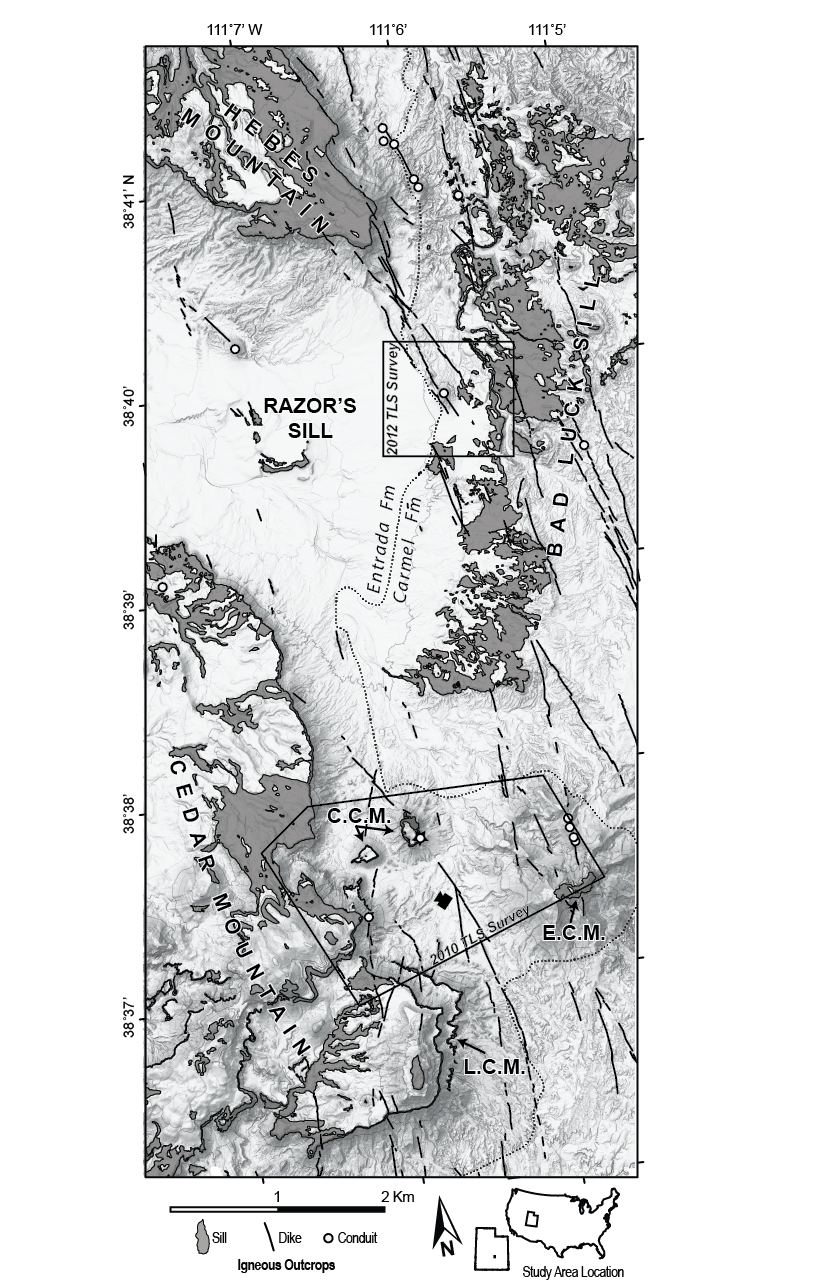
\includegraphics[width=0.4\linewidth]{\FigPath/Fig1-map}
\caption[Shaded relief map of airborne laser scanning data, San Rafael Swell, Utah (USA) with formation contact and terrestrial laser scanning (TLS) areas labeled]{Shaded relief map of airborne laser scanning data, San Rafael Swell, Utah (USA) with formation contact and terrestrial laser scanning (TLS) areas labeled. Sills mapped are Hebes, Bad Luck, Razor’s, Cedar Mountain, Lower Cedar Mountain (LCM), Central Cedar Mountain (CCM), and East Cedar Mountain (ECM). Starred conduit symbol near CCM denotes conduit that was formed concurrently with CCM sill. Camera symbol near CCM is view location of Figure \ref{fig_panorama}.}
\label{fig_map}
\end{figure}

\section{Geologic description}

The San Rafael volcanic field was active between 4.6 and 3.8~Ma \citep{delaney1997physical}. This volcanic field is part of a larger occurrence of Cenozoic basaltic volcanism in the Colorado Plateau and Basin and Range provinces but is distinct from many other fields as it has been eroded to a depth of $\sim$800~m, based on its age and late Cenozoic erosion rates \citep[e.g.]{pederson2002colorado}. The sill-and-dike swarm, or volcanic plumbing system, cut a Jurassic sedimentary section from the Carmel Formation through the Cutler Formation. Diabasic dikes in this area trend 335$^{\circ}$ to 0$^{\circ}$ (relative to north) along regional joint sets, indicating low horizontal deviatoric stress during emplacement \citep{delaney1997physical}. Sills in the San Rafael Swell range from $<$5~m to $>$40~m thick and are exposed in cliff sides and canyons in outcrops that extend for 100s-1000s~m. This shallow magma plumbing system has been mapped \citep{delaney1997physical}, and used to improve our understanding of (i) dike emplacement \citep{delaney1986field}, (ii) magma diapirism in the shallow crust \citep{diez2009evidence}, and (iii) the spatial relationships between dikes and conduits \citep{kiyosugi2012relationship}, the latter of which are commonly surrounded by brecciated country rock, indicating conduit erosion during rapid magma ascent. Although \citet{gartner1986geometry} described physical characteristics of exposed sills in the area, the complex emplacement processes of sills in this volcanic field have remained enigmatic. With the aid of lidar, we are able to document the complex map relationships between intrusions in the area.

\section{Lidar reconnaissance and analysis}\label{sec_lidarrec}

Terrestrial laser scanning (TLS), performed in 2010 and 2012, collected a 7.3 GB point cloud over an area of 5 km$^2$. Both TLS surveys used Riegl terrestrial scanners. An airborne laser scanning (ALS) survey, in 2013, provided data for a 54 km$^2$ airborne laser swath map (ALSM) \citep{richardson2013alsm}, connecting the 2 TLS surveys into a single study area (Figure \ref{fig_map}). Instrument specifications and data formats from these surveys are outlined in Table \ref{tab_specifications}. Co-registering the coordinate systems of the three surveys creates a coverage area of $\sim$50~km$^2$, within which relief varies by up to 500~m. Thus, we are able to characterize the magma plumbing system in a tabular block approaching 25 km$^3$ in volume, which bounds the study area extent. This reconstruction of a magmatic plumbing system attempts to model the amount of magma emplaced into the crust due to Pliocene volcanism for the 25~km$^3$ space.

\begin{table}[h]
\centering
\caption{Lidar Survey Specifications}
\begin{tabular}{l p{2.5cm} c p{3cm} c p{2.3cm}}
\toprule
Survey Date & Instrument & Camera & Instrument  & Points & Data Format \\
&&& Accuracy/Misfit$^*$ & per m$^2$ &\\
\midrule
June 2010	&	Riegl \mbox{LMS-Z620}	&	Nikon D200	&	10 mm/13 cm standard misfit between tiepoints	&	49	&	XYZRGBI ASCII \\
May 2012	&	Riegl VZ-400	&	Nikon D200	&	5 mm/11 cm standard misfit between tiepoints	&	148	&	XYZRGBI ASCII \\
August 2013	&	Optech Gemini ALTM	&	N/A	&	5-35 cm/5cm interswath misfit	&	
6.25	&	LAS \\
\bottomrule
\multicolumn{6}{p{0.95\linewidth}}{$^*$ Misfit in Riegl point clouds are reported after Georeferencing to WGS84 in RiSCAN Pro 1.8.0.}\\
\end{tabular}
\label{tab_specifications}
\end{table}

The three point clouds (two TLS and one ALSM) were consolidated and analyzed using LiDAR Viewer software \citep{kreylos2008immersive}. Because the three-dimensional point cloud is so precise, lidar data help identify subtle changes in sill thickness over large areas, vertical offsets in sills, and disrupted stratigraphy in overlying sedimentary units, which allow magma movements to be deduced. Contacts between igneous and sedimentary rocks are identified by shade contrast (igneous rocks are generally darker than sedimentary rocks in the near-infrared point cloud) and weathering patterns easily observable in the point cloud (Figure \ref{fig_photo-pcloud}). Thickness measurements are made in LiDAR Viewer where sill upper and lower contacts are seen in close proximity. The exact locations of sill contacts are manually picked between points in the point cloud, where one point is interpreted as sill and the other as sedimentary rock (Appendix \ref{apdx_lidar}). Uncertainty at each measurement is determined as the average of point-to-point distances on top and bottom of the sill and is drastically reduced in areas where both TLS and ALSM data are available. Other measurements made in LiDAR Viewer include sill base elevations and strikes and dips of continuous sill segments and of sedimentary host rock below sills. Locations where sills abruptly change stratigraphic level are also mapped in the field. These abrupt changes can be traced between outcrops with point cloud measurements.

Sill exposures are mapped using 1~m National Agriculture Imagery Program (NAIP) images and the ALSM digital elevation model (DEM). These are combined with thickness measurements to estimate terminal boundaries of sills. The lateral edges of sills are not commonly preserved in outcrop, so we have estimated the terminal boundary of each sill to extend no more than 0.5~km from current exposures. Sills commonly crop out at cliffs with little horizontal exposure area (Figure \ref{fig_panorama}), and by assuming that the mapped sills are contiguous between these outcrops, mapped sill areas are relatively small in comparison to interpreted sill areas (Table \ref{tab_mappedmodeled}). Sill volume and average thickness are modeled by constraining the thicknesses of sills at their respective modeled boundaries to be 0~m and interpolating a Laplacian-spline surface within sill boundaries, calibrated to the measured thicknesses (Figures \ref{fig_twomodels} and \ref{fig_fivemodels}). Results from mapped and modeled areas, and maximum measured thicknesses, are detailed in Table \ref{tab_mappedmodeled}.

Using aerial images and field mapping, \citet{kiyosugi2012relationship} mapped 16 conduits and ~180 vertical, en echelon dike segments, with a cumulative length of ~53 km, that crop out in the study area (Figure \ref{fig_map}). The cumulative volume of igneous material stored in dikes is estimated to be the product of dike length, the modeled block height, and 85 cm, the modal dike thickness \citep{delaney1997physical}. This might be a slight overestimate as some dikes might not have cut through the entire block height. The volume stored in conduits is the product of the surface area, mapped with the ALSM DEM and NAIP images, of each conduit and the modeled block height. This assumes conduit thickness does not change within the vertical limits of this reconstruction and might underestimate volume if conduits widen toward the surface or formed above the present-day surface.

\section{Igneous system reconstruction}

\begin{figure}
\centering
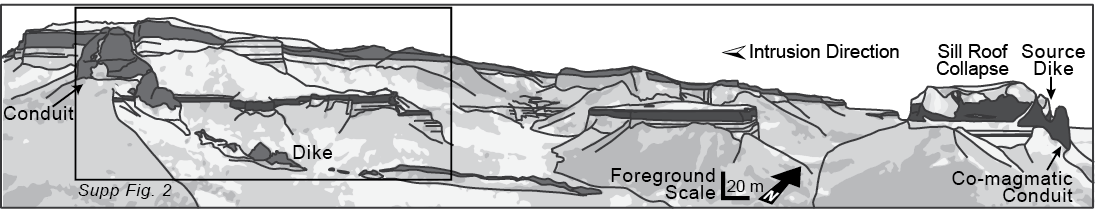
\includegraphics[width=\linewidth]{\FigPath/Fig2-panorama}
\caption[Northwest-facing panoramic diagram of Central Cedar sill, shaded dark gray (see Figure \ref{fig_map} for location)]{Northwest-facing panoramic diagram of Central Cedar sill, shaded dark gray (see Figure \ref{fig_map} for location). Other igneous intrusions are lighter gray, including sill capping Cedar Mountain (background), a conduit, and a dike.}
\label{fig_panorama}
\end{figure}

\begin{table}
\centering
\caption{Areas, Thickness, and Volumes for 7 Sills in the Eroded San Rafael Swell Volcanic Field}
\begin{tabular}{p{3cm} c c | c c c}
\toprule
 & \multicolumn{2}{c}{Observations} & \multicolumn{3}{c}{Modeled values} \\ 
\midrule
 Sills & Mapped area$^*$ & Max  & Modeled area & Volume & Mean\\ 
 & (10$^3$ m$^2$) & thickness$^*$ & (10$^3$ m$^2$) & (km$^3$) & thickness\\
\midrule
Bad Luck & 2901$\pm$141 & 19.0$\pm$0.2~m & 13040 & $9.45\times 10^{-2}$ & 7.3~m\\ 
Cedar Mountain & 2782$\pm$149 & 40.7$\pm$0.2 & 25570 & $2.78\times 10^{-1}$ & 10.9 \\
Hebes & 1919$\pm$45 & 36.1$\pm$0.1 & 5390 & $8.47\times 10^{-2}$ & 15.7\\ 
East Cedar Mountain & 39$\pm$2 & N/A$^{\dag}$ & 130 & $4.08\times 10^{-4}$ & 3.0\\ 
Razor's & 37$\pm$4 & 7.8$\pm$0.2 & 1270 & $1.62\times 10^{-3}$ & 1.3\\ 
Central Cedar Mountain & 26$\pm$5 & 15.5$\pm$0.1 & 880 & $4.42\times 10^{-3}$ & 5.0\\ 
Lower Cedar Mountain & 20$\pm$5 & 14.4$\pm$0.2 & 1030 & $5.44\times 10^{-3}$ & 5.3\\
\bottomrule
\multicolumn{6}{p{0.95\linewidth}}{$^*$ Area uncertainty determined by assuming a 1-pixel-width error in mapping with 1-m basemap image. Thickness uncertainty calculation is discussed in the text.}\\
\multicolumn{6}{p{0.95\linewidth}}{$^{\dag}$ Sedimentary rocks are not observed above East Cedar Mountain Sill, inhibiting thickness measurements.}\\
\end{tabular}
\label{tab_mappedmodeled}
\end{table}

Seven isolated sills crop out within the study area. We interpret these sills to have been emplaced independently as a result of single dike injections, based on evidence described below. Sill volumes range from 10$^{-4}$-10$^{-1}$ km$^3$ and have been emplaced over areas of 10$^{-1}$ to tens of square kilometers (Table \ref{tab_mappedmodeled}). Through modeling sill geometries, we find that $\sim$0.4 km$^3$ of igneous material is permanently stored in the sills, representing 93\% of all intrusive rocks in our reconstructed volume. Table \ref{tab_contribs} summarizes mapped areas and modeled volumes of sills, dikes, and conduits within the study area. By combining adjacent conduits along the same dike, we estimate that 12 distinct volcanic events are represented within the study area. Emplacement processes of sills and their role in the development of the Pliocene volcanic field can be further understood by investigating individual sills.


\begin{figure}
\centering
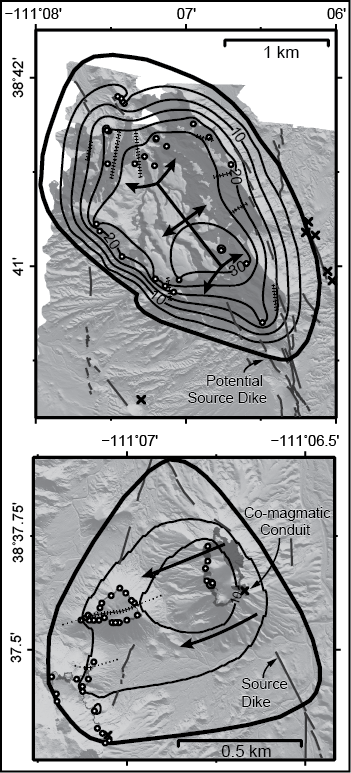
\includegraphics[width=0.4\linewidth]{\FigPath/Fig3-models}
\caption[Sill thickness contour plots of Hebes and Central Cedar sills]{Sill thickness contour plots of Hebes (top) and Central Cedar (bottom) sills. White circles show measurement locations; X symbols are mapped conduits; gray lines are dikes; shaded areas are mapped sills. Thick lines with arrows indicate inferred direction of magma injection; hashed and dotted lines indicate mapped and inferred vertical sill offsets, respectively. Thick contours mark modeled sill boundaries where thickness is modeled to be 0~m.}
\label{fig_twomodels}
\end{figure}

\subsection{Hebes Sill}

The sill at Hebes Mountain (Figure \ref{fig_map}) is primarily preserved as a single 1.9 km$^2$ sill exposed over an area of $\sim$4~km$^2$. This sill generally dips with strata 1$^{\circ}$-8$^{\circ}$ to the northwest, although locally some areas dip 5$^{\circ}$-30$^{\circ}$ toward the center of the sill. Sill thicknesses are measured to a precision of $\pm$75~cm, with virtually all exposures measuring $>$19~m. The sill thins monotonically from the center to the edges of Hebes Mountain, thinning most rapidly to the southwest.

By modeling Hebes sill as a 5.4~km$^2$ area, roughly following the shape of Hebes Mountain, the volume is estimated to be $8.5\times 10^{-2}$ km$^3$. The elongate nature of this sill model (Figure \ref{fig_twomodels}), with increased thickness trending in the northwest dip direction is aligned in the regional dike direction, perhaps indicating a linear source region (dike) feeding the sill.

\subsection{Central Cedar Sill}

\begin{figure}
\centering
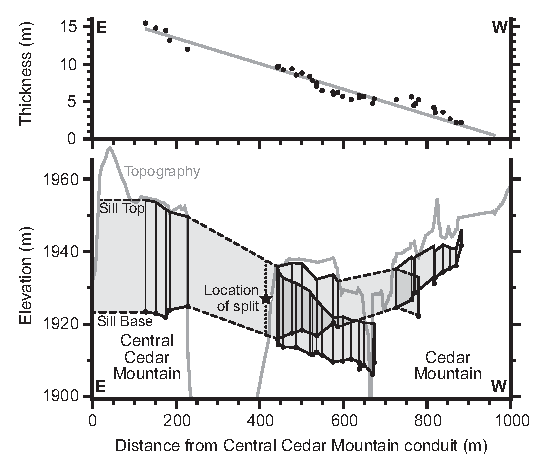
\includegraphics[width=0.5\linewidth]{\FigPath/Fig4-chart}
\caption[Chart of measured thicknesses and elevations of Central Cedar sill]{Chart of measured thicknesses and elevations of Central Cedar sill. Top: Measured thicknesses of Central Cedar sill with respect to distance from conduit on Central Cedar Mountain with superimposed linear trend. All vertical errors are within size of plotted points. Bottom: Pseudo–cross section of Central Cedar sill superimposed on current topographic profile. Filled circles represent measured basal elevation (m above sea level) of sill; shaded area represents interpolated sill. Dotted line (star symbol) is inferred location where sill splits into two branches, manifested as step-ups in outcrop.}
\label{fig_chart}
\end{figure}

The Central Cedar sill caps two buttes to the east of Cedar Mountain and is exposed on the east facing cliffs of Cedar Mountain (Figure \ref{fig_panorama}). The outcrops are interpreted to be parts of a single sill, as their basal contacts project across the small valleys between each exposure at the same elevation. Measured thicknesses of the Central Cedar Sill are 2-15 m, with basal contacts that dip with sedimentary host rock, at 2-5$^{\circ}$ WNW to SW. The sill outcrops adjacent to a conduit associated with a $\sim$2~km long dike on Central Cedar Mountain. Basalt between the conduit and sill appears continuous, with no brecciation, suggesting the dike and sill were formed cotemporally, and were thus comagmatic.

The average uncertainty in thickness measurements for Central Cedar Sill is $<$20 cm, due to coverage from both ALSM and TLS data sets. The point cloud also enables the mapping of curvilinear ``step-up'' features, defined by \citet{gartner1986geometry} as vertical offsets between different intrusion pathways, or feathers. Flow direction during intrusion is interpreted to be parallel to step-ups. Step-ups in this sill indicate flow to the W-WNW, away from and/or toward, the conduit. Modeling this sill as a tongue-shaped body intruding to the west from the suspected source dike (Fig S1, top center), Central Cedar Sill has an areal extent of $\sim$0.88~km$^2$, and a total volume of $4.4\times 10^{-3}$~km$^3$ (Table \ref{tab_mappedmodeled}).

A linearly thinning trend away from the conduit is evident in the sill, continuing for 1~km to the observed sill limit (Figure \ref{fig_chart}). Within 100~m of the conduit, sill thickness changes dramatically due to the presence of rotated sandstone blocks with thin basalt lenses injected over the tops of the sandstone blocks, indicating roof collapse into the sill (Figure \ref{fig_panorama}). From these observations we conclude that the Central Cedar Sill was fed from a single dike and was emplaced in a tongue-like fashion to the west in its initial dipping direction. Further, we infer that a conduit-forming volcanic event may have halted further advance of the sill and subsequent flow of magma from the sill into the conduit caused the observed conduit-adjacent roof collapse.

\begin{table}
\centering
\caption{Igneous Material Contributions in the Study Area}
\begin{tabular}{l c c c}
\toprule
 & Area (km$^2$) & Volume  & Vol\% of  \\
 & & (km$^3$) & intrusives \\
\midrule
 Sills & 34.5 & $4.1 \times 10^{-1}$ & 92.9 \\ 
 Dikes & $4.5 \times 10^{-2}$ & $2.2 \times 10^{-2}$ & 5.0 \\
 Conduits & $1.9 \times 10^{-2}$ & $9.5 \times 10^{-3}$ & 2.1 \\
 Total & 34.6 & $4.5 \times 10^{-1}$ & 1.8 \\
 Model Space & 50.0 & 25.0 & --- \\
\bottomrule
\end{tabular}
\label{tab_contribs}
\end{table}

\section{Discussion and conclusions}

Through lidar mapping of the San Rafael study area, seven sill-forming events in the shallow crust and 12 conduit-forming events have been identified and mapped in detail (Figure \ref{fig_map}). We model the total volume of igneous material stored in sills to be 0.4~km$^3$ within a 25~km$^3$ block. This sill volume represents 93\% of the stored igneous volume in the block, with the remaining 7\% in dikes and conduits. There is no doubt that, volumetrically, sills are a critical component of the magma plumbing system in this distributed volcanic field.

\begin{figure}
\centering
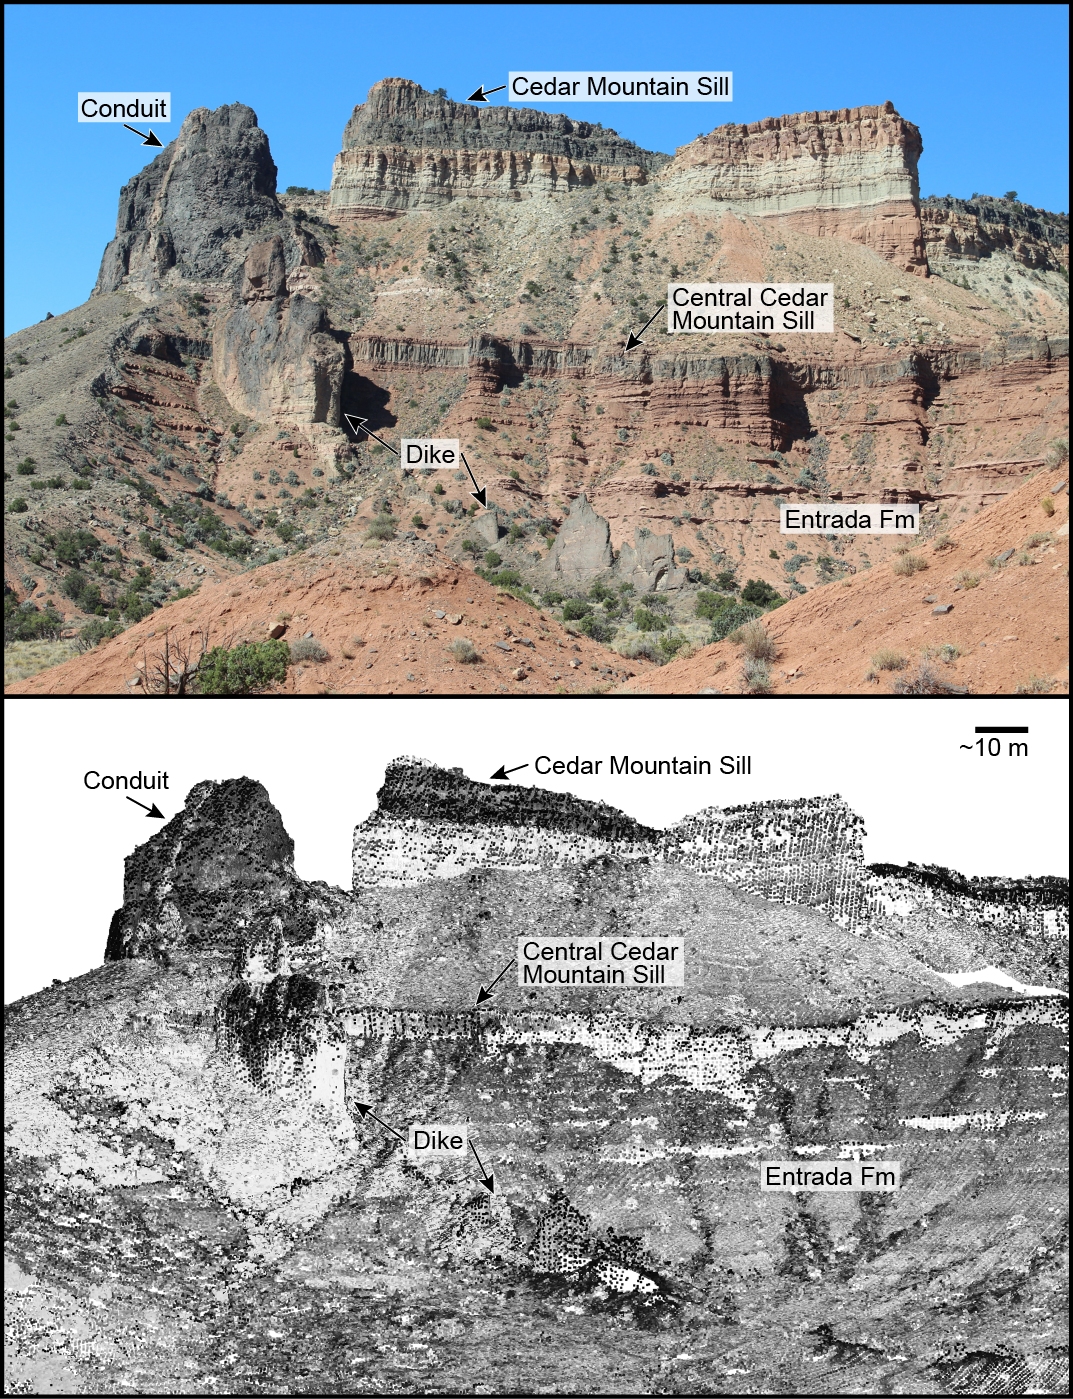
\includegraphics[width=0.7\linewidth]{\FigPath/SFig2-photo_pcloud}
\caption[Photograph and lidar point cloud of Cedar Mountain]{Photograph and lidar point cloud of Cedar Mountain. Top: Photograph of the east face of Cedar Mountain featuring Central Cedar Sill, Cedar Mountain Sill, and a dike which cross-cuts Central Cedar Sill. Sills are separated by dozens of meters by sedimentary rock. Photograph courtesy of J. McIlrath. Bottom: Combined TLS and ALS point cloud of the same view. Near-Infrared intensity differentiates between igneous and sedimentary rocks.}
\label{fig_photo-pcloud}
\end{figure}

It is possible, in fact, that sill volume in the San Rafael Sell volcanic field is comparable to erupted volume. Eruption volumes for the 12 conduits cannot be directly observed, as those lavas are completely eroded away. Eruption volumes for monogenetic volcanoes in similar fields span three orders of magnitude, ranging from 10$^{-3}$ to 10$^{-1}$~km$^3$ \citep[e.g.]{crowe1983aspects, condit1989patterns, kiyosugi2012relationship}. If we assume that average eruption volume is 0.1 km$^3$ for conduits in the San Rafael Swell, $\sim$1.2 km$^3$ of basalt would have been erupted at the surface, four times the estimated sill volume. Again, this comparison suggests that, volumetrically, crustal storage of magma in sills is a major feature of the magmatic system.


\begin{figure}[h!]
\centering
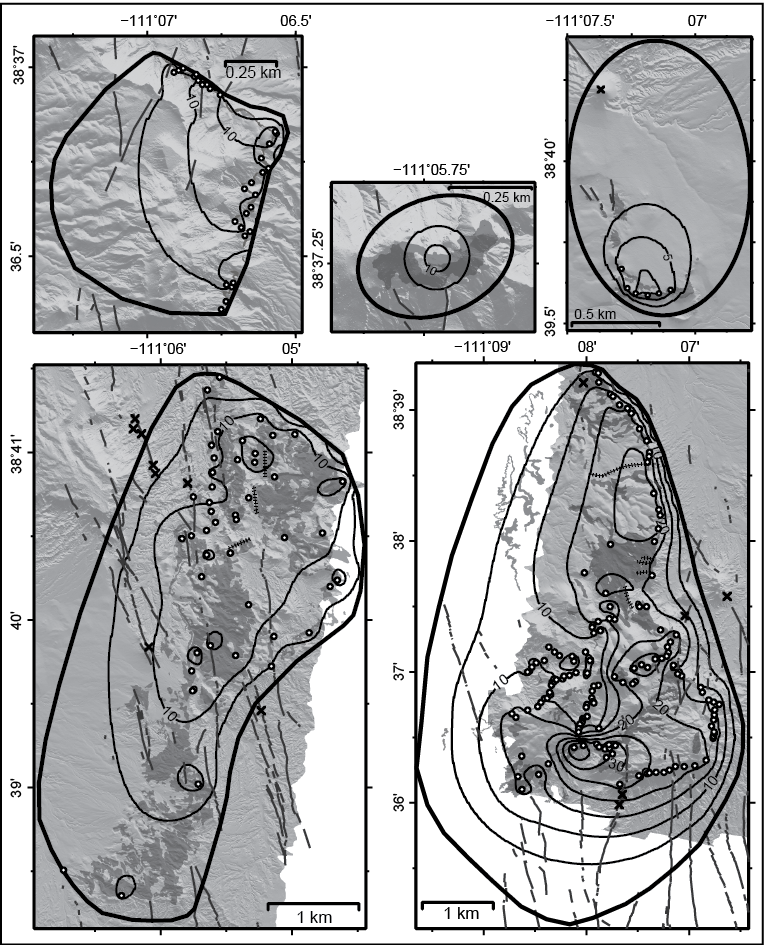
\includegraphics[width=0.7\linewidth]{\FigPath/SFig1-5models}
\caption[Contour plots of thickness models over ALSM hillshade data for additional sills]{Contour plots of thickness models over ALSM hillshade data for additional sills. White circles are measurement locations; Xs are mapped conduits; gray lines are dikes; shaded areas are mapped sills. Thick lines with arrows indicate the inferred direction of magma injection and hashed/dotted lines indicate mapped/inferred vertical sill offsets. Top row, left to right sills are: Lower Cedar, East Cedar Mountain, Razor's; Bottom row, left to right: Bad Luck, Cedar Mountain. Contour intervals are 5~m thickness except Razor’s sill where contours are every 2.5~m. Thick contours mark the modeled sill boundaries where sill thickness is modeled to be 0~m thickness. Note change in map scale. }
\label{fig_fivemodels}
\end{figure}

The general shape of the mapped sills in this field does include a thick center of several to tens of meters in height, tapering edges, and horizontal dimensions of one to several kilometers. While smaller sills exhibit a monotonic decrease in thickness from their interiors (Figure \ref{fig_chart}), the thickness profiles of larger sills are more complex and multiple thickened zones exist (Figure \ref{fig_fivemodels}). The irregular shapes and size range of these sills might suggest that all sills in this area are the product of single injection events and are not polygenetic \citep{gudmundsson2012magma}. Furthermore, the maximum observed thicknesses of each of these sills are not highly correlated to the exposed or modeled areas of each sill. Sills in this area generally ascend stratigraphy only after lifting the roof, enabling exploitation of new bedding planes, suggesting that initial emplacement at this depth was a pressure-driven process, similar to the intrusion of the Trachyte Mesa laccolith (Henry Mountains, Utah, USA) \citep{wetmore2009geometry}. Because horizontal deviatoric stress was low in this area during the Pliocene \citep{delaney1986field}, the minimum compressive stress direction could have significantly migrated from horizontal at 1 km depth, enabling sill formation given local stress conditions influenced by overlying topography \citep{gudmundsson2012magma}.


The development of shallow sills likely affected eruption dynamics. If a comagmatic sill is present during a volcanic eruption, ascending bubbles can become concentrated in the vertical conduit at the conduit-sill junction by disproportional capture of the liquid phase of a two-phase flow in the horizontal branch \citep{conte2000experimental}. This concentration occurs if overall magma flux is sufficiently low. The presence of the sill, therefore, enables modulation of explosive potential, with low magma flow rates resulting in more explosive activity than if a sill was not present. Following the method of \citet{pioli2009controls}, assuming a magma density of 2800~kg/m$^3$, we calculate the transition flux to be $1.8\times 10^5$~kg/s within the Central Cedar Mountain conduit (diameter 25~m), where lower flux would have concentrated bubbles in the conduit system. As average mass eruption rate for strombolian eruptions is commonly observed to be 10$^3$-10$^5$ kg/s \citep{pioli2009controls}, the presence of sills at the level where H$_2$O exolves critically impacts volcanic hazard.

Sills have been identified as a major instigator of unrest in association with stratovolcanoes \citep[e.g.]{biggs2010stratovolcano,tarasewicz2012magma}, volcanic calderas \citep{macedonio2014sill}, and monogenetic volcanic eruptions \citep{erlund2010compositional}. The observation in the San Rafael Swell that the vast majority of igneous rock at ~1 km depth is contained in sills suggests that similar deformation events may be precursory to volcanic eruptions in some active volcanic fields. Monitoring of active volcanic fields may benefit from use of deformation networks to detect sill emplacement in the shallow crust.



\section{Acknowledgments}
This project would not have been possible without the support of David Phillips and UNAVCO for lidar field equipment and data processing assistance. The TLS data acquisition project was funded by a grant from the National Science Foundation (EAR-0910696). ALS data acquisition and processing was completed by the National Center for Airborne Laser Mapping (NCALM) with funding provided by NSF’s Division of Earth Sciences, Instrumentation and Facilities Program (EAR-1043051). M. Oskin and O. Kreylos of UC Davis are thanked for their help regarding LiDAR Viewer. USF students and faculty, Judy McIlrath, Kaz Mannen, Koji Kiyosugi, James Wilson, Samantha Kinman, and Travis Doering are thanked for field assistance. Helpful comments from K. Cashman, A. Gudmundsson, and an anonymous reviewer improved this manuscript.

%%%%%%%%%%%%%%%%%%%%%
%%References Section
%\section{References}

%\nobibliography{dissertation_refs}
%\bibliographystyle{apalike} 

\chapter[Validating Lava Flow Simulators using a Validation Hierarchy and Bayesian Analysis]{Validating Lava Flow Simulators using a Validation Hierarchy and Bayesian Analysis}

%compile with pdflatex:
%:! bibtex %:r
%:! pdflatex -synctex=1 -interaction=nonstopmode --shell-escape %

\renewcommand*{\FigPath}{../Chapter-molasses/figures}

\section*{Abstract}
	Modeling lava flows through cellular automata (CA) methods enables a computationally inexpensive means to quickly forecast lava flow paths and ultimate areal extents. A CA program has been created in the program language C that is modular, which enables a combination of governing CA rules to be evaluated against each other. My objective is to find a successful combination of automata behaviors that behaves like a bingham fluid and accurately forecasts lava inundation. To fulfill this objective, four validation levels have been devised, into which different benchmarks can be applied to test lava spreading algorithms against increasingly complex tests. These levels are 1) verification of the code by testing for conservation of mass; 2) testing for flow self-similarity given inconsequential variations in input parameters; 3) testing for replication of Bingham flow morphology on simple surfaces; and 4) testing for replication of real lava flow morphologies on pre-eruption elevation models. Two Bayesian posterior statistics $\text{Pr}(Lava|Sim)$ and $\text{Pr}(\neg Lava|\neg Sim)$ are then used to further charactarize model performance against the 2012-3 Tolbachik lava flow. These metrics can provide insight into improving model performance and decision making in volcanic crises.

\section{Introduction}
	Lava flows as a gravity current on the surface of the Earth when liquid magma is effused at the surface with little or no explosivity. In the vacinity of active volcanoes, lava flows represent significant long term impact to infrastructure \citep{peterson2000lava}. In the past, lava flow hazard has been mitigated with the construction of physical diversions and at least once in 252 A.D. by the supernatural grace of St. Agatha of Sicily who died the year prior. Modern science suggests, however, that forecasting the flow path of lava from active volcanoes might be more useful than St. Agatha for communities impacted by effusive volcanism.

	Methods of forecasting lava flows range from simple predictions using empirical relationships between magma flux and flow length \citep{Glaze2003}, to 1-D numerical solutions such as FLOWGO \citep{harris2001flowgo}, to advanced computational fluid dynamics codes like lavaSIM \citep{hidaka2005vtfs}. All modern numerical flow models by nature trade precision in simulating physical processes with computer run-time, so that while FLOWGO is relatively fast it only predicts downslope flow length, while lavaSIM solves Navier-Stokes equations to produce a 3-D flow distribution at the expense of large computational requirements.
	
	Cellular Automata (CA) methods have been developed to simulate fluid flow, including lava spreading \citep{barca1994cellular}. In contrast to CFD codes, these do not generally attempt to compute Navier-Stokes equations but instead abstract many physical parameters, such as viscosity and temperature, into more or less empirical rules. The benefit of CA methods for simulating lava flows is most noticeable in the reduced computer time necessary for simulation compared to CFD methods.
	
	Multiple CA lava flow algorithms exist, such as SCIARA \citep{crisci2004simulation}, MAGFLOW \citep{del2008simulations}, ELFM \citep{damiani2006lava}, and LavaPL \citep{connor2012}. These algorithms are variations on a theme, where the largest difference between each is how lava is distributed from one automaton to its neighbors. For instance, three versions of SCIARA allow for lava to spread in cardinal directions \citep{barca1994cellular}, in hexagonal directions \citep{crisci2008lava}, or in directions based on an inherent velocity calculated in an eulerian way for each automaton \citep{avolio2006sciara}. MAGFLOW and ELFM by contrast to the original SCIARA algorithm implements 8 directions of spreading. LavaPL and SCIARA both spread in four directions but the apportionment of lava from one automaton to neighbors is based on a different algorithm.

	While several lava flow simulators now exist, each have been made and tested with different lava flows or aspects of flows in mind. Because of this, selecting a specific algorithm to effectively model lava flow hazards can be a necessary, if unwanted challenge. To address this problem, we propose a hierarchical validation scheme to objectively test different flow spreading algorithms. Benchmark tests can be designed with different validation levels in mind, to compare lava flow simulations to increasingly complex models, from simply conserving mass to replicating the paths and ultimate areal extents of real lava flows. The benchmarks described in this project can be applied to any flow algorithm that provides at least a list or map of inundated locations over various topographies.

	In this paper, multiple lava flow algorithms are tested using a new modular lava flow code, which I have named MOLASSES (standing for \textit{MOdular LAva Simulation Software in Earth Science}). This code, implemented in C, is a Cellular Automata code which tracks a population of equal-area spaced cells over a grid, that is defined by a digital elevation model (DEM). These cells may or may not be inundated with lava and they are governed by universal rules. Because MOLASSES has been designed in a modular way, it is relatively quick to modify the flow algorithm. Using this code while changing methods of lava distribution enables code output in a constant format, which simplifies the comparison of methods.
	
	In Section \ref{sec:MOLASSES}, I will demonstrate how CA is applied to lava flows and detail how a CA simulation is carried out in the MOLASSES code. I will introduce a validation hierarchy in Section \ref{sec:benchmark} that can be used to verify and validate different lava flow algorithms using increasingly complex model parameters. In Section \ref{sec:Bayesian}, I will expand on the final validation level (validation against real lava flows) with a Bayesian approach to improving model performance for the 2012-3 Tolbachik Lava Flow. The results from these Sections will be discussed in Section \ref{sec:discussion}.
	
	\subsection{Case Study Area: 2012-3 Tolbachik Lava Flow}\label{sec_tolb_back}
	In the third validation level (Section \ref{sec_tolb_bench}), the recent lava flows at Tolbachik will be used as an example benchmark test to validate flow algorithms against a real lava flow. These flows will then be used in Section \ref{sec:Bayesian} as examples of how a Bayesian approach to evaluating model performance can improve model performance. 
	
\begin{figure}[!h]
	\centering
	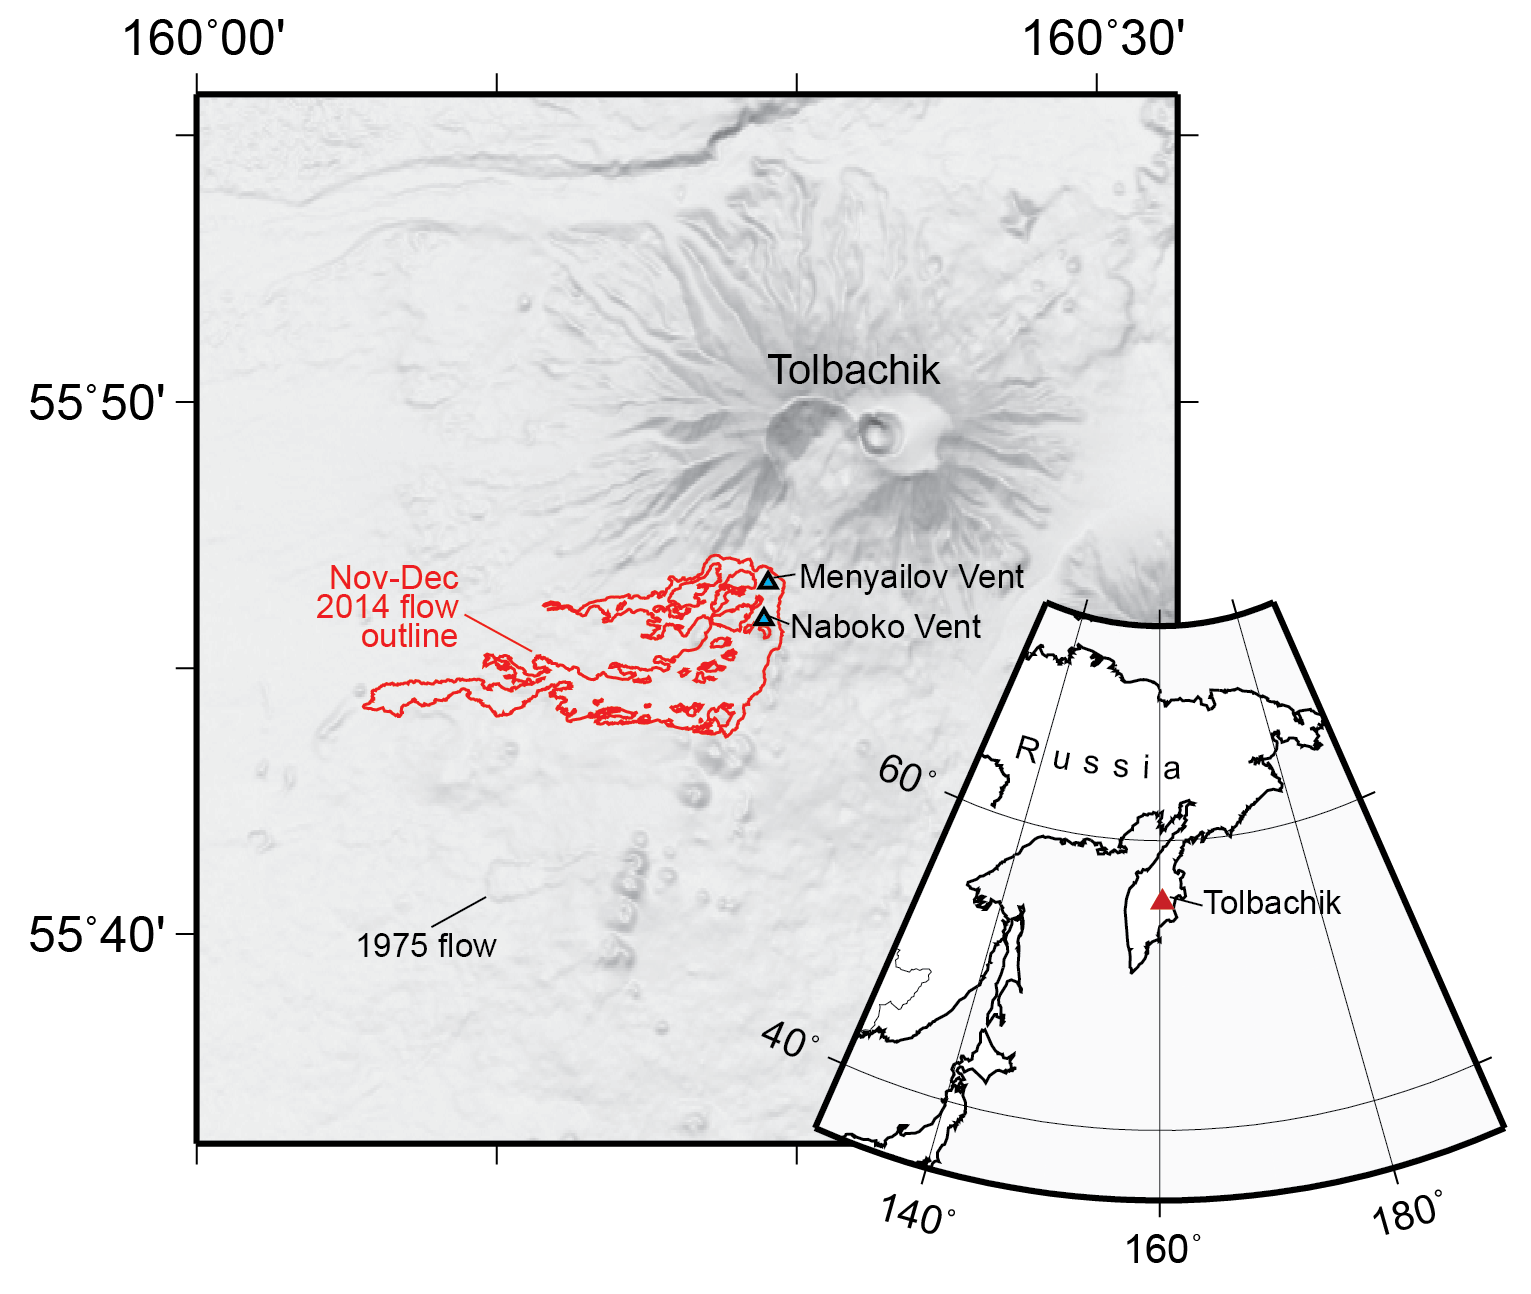
\includegraphics[width=0.7\linewidth]{\FigPath/locator_complete_300dpi}
	\caption[The Tolbachik region of Kamchackta, Russia]{The Tolbachik region of Kamchackta, Russia. The two main vents are shown as triangles and the outline of western lava flows, emplaced in 2014, is drawn in red.}
	\label{fig_locator}
\end{figure}
	
The Tolbachik lava flow began in November 2012, originally being sourced from a long fissure vent south of Tolbachik Dol. Initial magma flux was estimated to be 440~m$^3$~s$^{-1}$ \citep{belousov2015overview}. The fissure vent ultimately coalesced into two main vents, seen in TanDEM-X interferometric synthetic aperture radar (InSAR) data \citep{kubanek2015lava}, and the flux dropped significantly to between 100 and 200~m$^3$~s$^{-1}$. Early stages of the flow carried lava west to a maximum runout of 14.5~km and later stages beginning in January or February, carried lava east. The total emplacement volume is $\sim$0.53$\pm$0.07~km$^3$ with 0.38~km$^3$ of that being to the west. TanDEM-X InSAR data has been used to show that the modal thickness of the flow is 7.8~m, and that the overall thickness distribution is log-normal \citep{kubanek2015lava}. After the flow ceased, the total emplacement area was mapped using orthophotos and TanDEM-X data where clouds were present in the images by \citet{kubanek2015lava}.

Figure \ref{fig_locator} shows the outline of the early lava flows, which traveled from two vents along a fissure to the west. This areal extent will be used to validate lava flow simulators. The flow volume is taken to be the total emplacement area within this outline, 26~km$^2$, multiplied by the observed modal thickness of the flow, 7.8~m. The total flow volume used the input parameter in the flow simulations will be 0.22~km$^3$. The remainder of the total emplacement volume to the west of the vents, 0.16~km$^3$ is interpretted to be material that built near-vent edifices (e.g. cones) \citep{kubanek2015lava}. The volume interpretted to be emminated from the northern vent is $4.63\times 10^7$~km$^3$, while the southern vent volume is $1.74\times 10^8$~km$^3$. This estimate was made by splitting the flow between areas north of the Menyailov (northern) vent and south of it, assuming that flows from the Menyailov vents traveled north.
	

%%%%%%%%%%%%%%%%%%%%%%%%%%%%%%%%%%%%%%%%%%%%%%%%%
%MOLASSES%%%%%%%%%%%%%%%%%%%%%%%%%%%%%%%%%%%%%%%%
%%%%%%%%%%%%%%%%%%%%%%%%%%%%%%%%%%%%%%%%%%%%%%%%%
%%%%%%%%%%%%%%%%%%%%%%%%%%%%%%%%%%%%%%%%%%%%%%%%%
%%%%%%%%%%%%%%%%%%%%%%%%%%%%%%%%%%%%%%%%%%%%%%%%%

\section{A Modular Cellular Automata Algorithm for lava flows}\label{sec:MOLASSES}

CA in lava flows has historically been defined as a 2-dimensional space, which is divided into equal-area grid cells, such as those found in a common digital elevation model (DEM). Within the location of each cell is defined an ``elementary automaton'' (\textit{ea}) that has a set of properties, is governed by a set of global rules, and has a set list of neighboring automata. While the behavior rules that each \textit{ea} follow is identical to those of all other automata, its behavior is only dictated by local phenomena. Specifically, the amount of lava that flows in or out of an \textit{ea} will depend on properties such as lava thickness and elevation within it and its neighbors. Because grid cells and \textit{ea} are fundamentally inseperable in this application, I will refer to \text{ea} as cells.

The set of cellular automata is defined as
	\begin{equation}
		\mathbf{A} = \mathrm{\{E^2, V, S, X, \sigma, \gamma\}}
	\end{equation}
	where E$^2$ is the set of point locations of cells in \textbf{A}, V$\subset$E$^2$ is the set of vent or source locations, S is the set of substates within each cell, and X is the local neighborhood that each cell can directly influence \citep{barca1994cellular}. $\sigma$ and $\gamma$ represent the transition functions and source functions within \textbf{A}. 
	
	Practically, E$^2$ is a set of coordinate pairs denoting row and column addresses of cells in a larger grid. S($i$,$j$), which represents the set of substates for the cell at row $i$, column $j$, includes S$_e$, the underlying elevation of an automaton; S$_h$, the thickness of lava within the cell; and S$_{h0}$, the critical thickness, above which lava will spread from a cell. Some algorithms include S$_T$, or the cell temperature in this set. X, in a four-connected neighborhood scheme, is given as \{(0,1), (0,-1), (1,0), (-1,0)\}, where (0,0) is the location of a cell under evaluation. $\sigma$ is the change of substates in S for each cell from timestep $t$ to $t+1$, or S$^{t}\rightarrow$S$^{t+1}$. $\gamma$ specifies the lava emitted at locations within V. The implementation of these sets within the CA structure \textbf{A} is described in detail below.
	
	\subsection{MOLASSES Algorithm Outline}
		MOLASSES is a Cellular Automata code developed in the C programming language based on the CA algorithm ``LavaPL'' of \citet{connor2012}. The major change between LavaPL and MOLASSES is that MOLASSES is constructed with nine modules that each have a specific task, either carrying out the CA simulation, reading model input, or writing model output (Figure \ref{fig_flowchart}). The nine modules were designed to replicated major functions in LavaPL and are:
		\begin{enumerate}
			\item{\textbf{DRIVER}} Calls modules in sequence to execute the flow algorithm.
			\item{\textbf{INITIALIZE}} Reads a user-provided configuration file to define model parameters.
			\item{\textbf{DEM\_LOADER}} Imports a raster file to define the elevation model.
			\item{\textbf{INITFLOW}} Uses model parameters to define data arrays.
			\item{\textbf{PULSE}} Incrementally adds lava to source locations.
			\item{\textbf{DISTRIBUTE}} Determines whether to spread and how to spread lava between cells.
			\item{\textbf{NEIGHBOR\_ID}} Identifies the cell neighborhood.
			\item{\textbf{ACTIVATE}} Adds newly inundated cells to the list of active cells.
			\item{\textbf{OUTPUT}} Writes model results to a file using user-specified formats.
		\end{enumerate}
		
		\begin{figure}[!h]
			\centering
			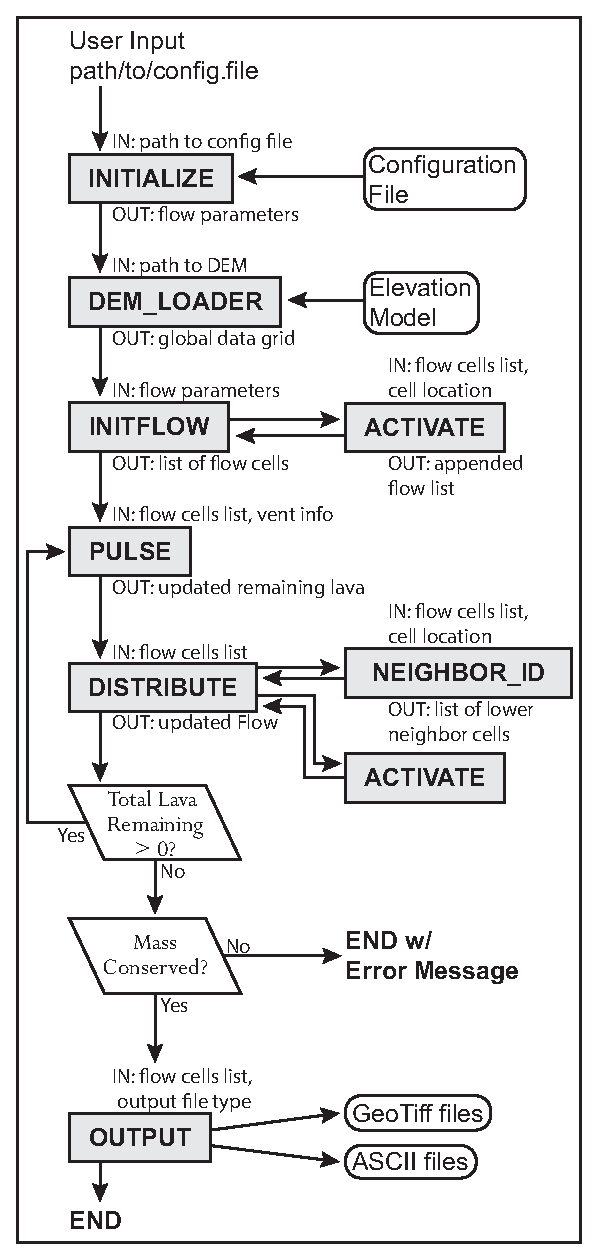
\includegraphics[width=0.3\linewidth]{\FigPath/Flow_Chart}
			\caption[MOLASSES flow chart]{A flow chart of MOLASSES carried out within the \textbf{DRIVER} module. Gray boxes denote various modules, with major inputs and outputs given above and below. Parallelograms are checks performed within DRIVER itself. Rounded boxes represent external input and output files.}
			\label{fig_flowchart}
		\end{figure}
		
		
		Like LavaPL, model parameters are specified by a user through a text configuration file, which must include 1) a digital elevation model (DEM), 2) a residual lava flow thickness, 3) at least one vent location, 4) the total volume and ``pulse volume'' of this vent, and 5) an output file path. The lava flow thickness defines the CA value of S$_{h0}$, where cells with flow thicknesses S$_h>$S$_{h0}$ will spread all lava to their neighboring cells, while cells with less lava will retain their lava. The ``pulse volume'' defines $\gamma$ and the amount of lava to emit at the source location at each time step. The total volume constrains $\gamma$ as lava will not be introduced to the source location after the total volume has been delivered. Modules within MOLASSES that further execute the CA simulation are detailed below.
		
	\subsection[Cells in E2]{Cells in E$^2$}
		%DEM_LOADER
		%INITFLOW
		%ACTIVATE
		Information for cells in the grid defined by E$^2$ is stored in two ways, for code efficiency. First, some information of the CA structure \textbf{A} is stored in a Global Data Grid. This grid stores information known at the beginning of the simulation, such as the user supplied residual flow thickness and the elevation. Grid dimensions are set in the \textbf{DEM\_LOADER} module to be identical to the user-specified raster DEM. This module then imports the elevation of each raster pixel into the corresponding grid cell location. After this operation, the residual flow thickness is also stored in the grid.

		The second information storage method is a list defined in the \textbf{INITFLOW} module. The ``Active List'' is declared with a length that corresponds to the theoretical maximum number of cells that can be inundated by lava. This list contains data that is updated during the simulation, including lava thicknesses, $S_h$, within cells. As cells are determined within the simulation to be inundated with lava for the first time, their row and column addresses, as well as their lava thicknesses are appended to the Active List with the module \textbf{ACTIVATE}.
		
	\subsection[Source Locations and the Source Function]{Source Locations, V, and the Source Function, $\gamma$}
		%INITFLOW
		%PULSE
		Initially in the Active List, \textbf{INITFLOW} only declares source location(s) as the first few elements of the list. These source locations are flagged in the list to be identified as source locations by other modules.

		The \textbf{PULSE} module carries out the source function, $\gamma$. In this module, a separate array stores each source vent's volume parameters. The pulse volume is added to the quantity of lava in the source cell and is subtracted from the remaining volume. The remaining volume is initially set as the total volume given in the configuration file, so PULSE continues to add lava to the source locations at each time step until remaining volume is 0.
		
	\subsection[Substates and the Transition Function]{Substates, S, and the Transition Function, $\sigma$}
		%INITFLOW
		%DISTRIBUTE
		Substates which cannot change, such as the cell elevation S$_e$ and the residual flow thickness S$_{h0}$, are stored within the Global Data Grid. Substates which do change, primarily flow thickness, S$_h$, are stored in the Active List and are allowed to change from timestep to timestep. These values are initialized in \textbf{INITFLOW} where thicknesses are set to 0.
		
		The transition function, $\sigma$, is defined in the \textbf{DISTRIBUTE} module. Cells in this module are evaluated in order of their inundation (i.e. vents are evaluated first and distal cells are evaluated last). The incoming and outgoing quantity of lava from each cell is stored in the Active List. Generally, if a cell has a flow thicknesses S$_h>$S$_{h0}$, it will spread the lava above S$_{h0}$ to any neighbors lower in elevation than itself. When all inundated cells have been evaluated, the incoming and outgoing quantities of lava of each cell are applied to the cells. This flow transition represents a timestep as all cells are updated at once.
		
		Multiple possible transition functions can effectively spread lava from and to cells in a manner that might replicate lava in real life. Selecting the best transition function is the purpose of the validation benchmarks described in Section \ref{sec:benchmark}. In this project three main variations are combined and tested which vary 1) how local slope affects spreading, 2) the neighborhood size, and 3) if any neighbors are eliminated from the neighborhood based on their relationship to the cell.
		
		\begin{figure}[!h]
			\centering
			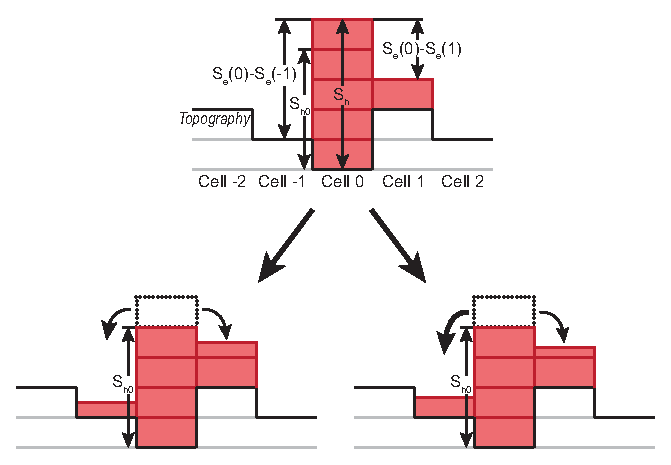
\includegraphics[width=0.5\linewidth]{\FigPath/slope-proportional-example}
			\caption[A 2-D example of two transition functions with different slope treatments]{A 2-D example of two transition functions. At timestep $t$ (top), Two cells are inundated with lava. The central cell (Cell 0) has 1 block of lava higher than the residual thickness, S$_{h0}$. In a slope-proportional sharing scheme, timestep $t+1$ will follow the path to the right; because Cell -1 has twice the relief as Cell 1, it receives twice as much of the residual lava (2/3 blocks vs. 1/3 to the right). In an equal-sharing scheme, the left path will be followed, and half the block will be added to both neighbor cells.}
			\label{fig_BernieSanders}
		\end{figure}
		
		\paragraph{Local slope-based spreading} In the LavaPL algorithm given by \citet{connor2012}, lava is apportioned from cells to their neighboring cells proportional to slope. To give a specific case, let a cell at location $c$ be the central cell, with a set of neighbor cells, X. The total relief between cell $c$ and its lower neighboring cells is 
		\begin{equation}
			\text{TR}(c) = \sum^{n\in \text{X}}(\text{S}_h(c)+\text{S}_e(c))-(\text{S}_h(n)+\text{S}_e(n))
			\label{eq_TR}
		\end{equation}
		where $\text{S}_h$ is the height or thickness of the lava in a cell, $\text{S}_e$ is the underlying elevation of the cell, and $n$ is a neighbor in X. The total lava to spread away from the central cell is the difference between thickness of lava (S$_h$) at $c$ the residual thickness (S$_{h0}$), unless the lava thickness is lower than the residual thickness, giving
		\begin{equation}
		 \text{Outbound}(c) =
			\begin{cases}
			\text{S}_h(c)-\text{S}_{h0}(c) & \quad \text{if } {S}_h(c)-\text{S}_{h0}(c) > 0\\
			0 & \quad \text{if } {S}_h(c)-\text{S}_{h0}(c) \le 0\\
			\end{cases}
			\label{eq_excess}
		\end{equation}
		
		In LavaPL, the excess flow, ``Outbound'', is delivered to neighbors $n$ based on the proportion of total relief, TR, found at each neighbor location (the right path of Figure \ref{fig_BernieSanders}). For each $n\in$X,
		\begin{equation}
			\text{Inbound}(n) = \text{Outbound}(c)\left(\frac{(\text{S}_h(c)+\text{S}_e(c))-(\text{S}_h(n)+\text{S}_e(n))}{\text{TR}}\right)
			\label{eq_propshare}
		\end{equation}
		This is the slope-proportional spreading equation. Another method would be ``slope-blind,'' and would spread lava to all lower neighbors equally following the equation
		\begin{equation}
			\text{Inbound}(n) = \left(\frac{\text{Outbound}(c)}{|\text{X}|}\right)
			\label{eq_equalshare}
		\end{equation}
		where $|\text{X}|$ is the size of the neighborhood, or the number of elements in the neighborhood. This is illustrated as the left path of Figure \ref{fig_BernieSanders}.
		
		\paragraph{Neighborhood size} The size of the neighborhood, X, in CA algorithms is commonly 4 or 8 in cardinal or ordinal directions. Here both have been implemented, which enables the benchmarks to test whether 8 spreading directions increases the performance of these tests. This is further described in the next section (\ref{sec_X}).

		\paragraph{Spreading inhibited by special relationships} Though the size of the neighborhood is set globally for all cells, neighbors are not guaranteed to receive lava from central cells. In all algorithms, for example, cells in the neighborhood that are higher than the central cell, including lava thicknesses, are excluded from the neighborhood set.
		
		\begin{figure}[!h]
			\centering
			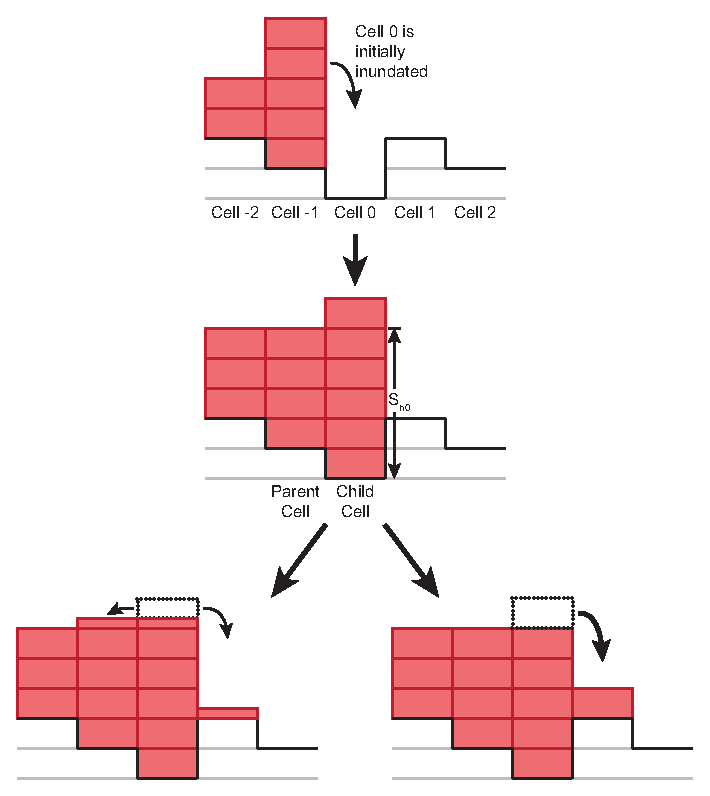
\includegraphics[width=0.5\linewidth]{\FigPath/parent-child-example}
			\caption[A 2-D example of different transition functions with different ``parentage'' rules]{Another 2-D example of different transition functions. In the first timestep (top), Cell -1 initially inundates Cell 0, creating the Parent-Child relationship shown in the next illustrated timestep (middle). If Parents cannot receive lava from Child cells, all residual lava in Cell 0 will flow to Cell 1, following the path to the right. If these relationships are ignored, as shown in the left path, Cell 0 will spread lava in both directions.}
			\label{fig_ParentTrap}
		\end{figure}
		
		Other neighbor elimination rules can also be implemented. One has been designed by \citet{connor2012}, where the cell that initially gives lava to another cell is forever eliminated from the receiving cell's neighborhood. This is done by creating a ``parent-child'' relationship for each activated cell in the flow. Simply put, child cells cannot give lava to their parent cells (right path in Figure \ref{fig_ParentTrap}). This transition function rule is tested against no parentage rules in competing MOLASSES algorithms (left path in Figure \ref{fig_ParentTrap}).
		
	\subsection{Cell Neighborhood, X}\label{sec_X}
	
	\begin{figure}[!h]
		\centering
		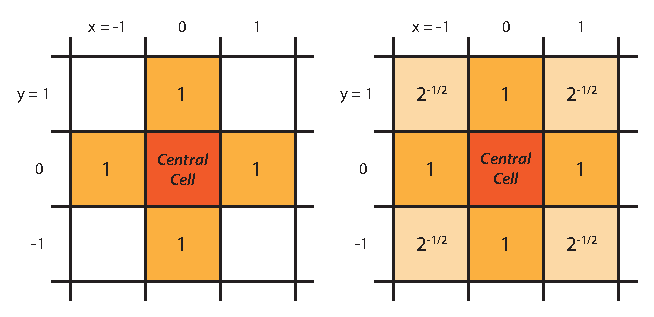
\includegraphics[width=0.5\linewidth]{\FigPath/neighborhoods}
		\caption[Cellular Automata neighborhoods]{Cellular Automata neighborhoods. To the left, in a 4-connected neighborhood, a central cell may influence or be influenced by cells in cardinal directions. To the right, in an 8-connected neighborhood, the zone of influence is expanded to include ordinal directions. Numbers in each cell are relative weights (determined by distance from the central cell), so diagonal neighbors are weighted less than orthogonal cells.}
		\label{fig_MrRogers}
	\end{figure}
	
		%NEIGHBOR_ID
		The final set in the CA is the cell neighborhood X and is defined by the \textbf{NEIGHBOR\_ID} module. This neighborhood is usually either 4-connected (von Neumann neighborhood) or 8-connected (Moore neighborhood) as illustrated in Figure \ref{fig_MrRogers}. Four-connected neighborhoods are defined as the row, column coordinates \{(0,1), (0,-1), (1,0), (-1,0)\}, where (0,0) is the location of a cell under evaluation, while the set elements might correspond to North, South, East, and West. Eight-connected neighbors include the ordinal directions, Northeast, Southeast, Northwest, and Southwest: \{(0,1), (0,-1), (1,0), (-1,0), (1,1), (-1,-1), (1,-1), (-1,-1)\}.
		
		NEIGHBOR\_ID is implemented within the DISTRIBUTE module to evaluate cells within X, and determine whether they are lower in elevation (including their lava) than the central cell. If one is lower, NEIGHBOR\_ID returns their relief, or the difference in elevation between the cell and the central cell, to the DISTRIBUTE module. Depending on whether parent-child relationships are recorded or ignored in the transition function, NEIGHBOR\_ID can follow one of two algorithms below.
		\begin{center}
		\begin{tabular}{l}
			\toprule
			\textbf{4-connected NEIGHBOR\_ID}\\
			\textbf{module}\\
			\midrule
			X = \{(0,1), (0,-1), (1,0), (-1,0)\}\\\\
			X' = \{\}\\
			$c$ = (0,0)\qquad (central cell location)\\
			\textbf{For} $n\in$ X\\
			~~\textbf{If}~$(\text{S}_h(c)+\text{S}_e(c))-(\text{S}_h(n)+\text{S}_e(n)) > 0$\\
			~~~~\textbf{Append}~$n$ to X'\\\\
			\textbf{Return}~X'\\
			\bottomrule
		\end{tabular}
		\begin{tabular}{l}
			\toprule
			\textbf{8-connected NEIGHBOR\_ID}\\
			\textbf{with Parent-Child Relationships}\\
			\midrule
			X = \{(0,1), (0,-1), (1,0), (-1,0), \\
			\qquad~(1,1), (-1,-1), (1,-1), (-1,-1)\}\\
			X' = \{\}\\
			$c$ = (0,0)\qquad (central cell location)\\
			\textbf{For} $n\in$ X\\
			~~\textbf{If}~$(\text{S}_h(c)+\text{S}_e(c))-(\text{S}_h(n)+\text{S}_e(n)) > 0$\\
			~~~~\textbf{If} $n$ is \textbf{not} Parent of $c$\\
			~~~~~~\textbf{Append}~$n$ to X'\\
			\textbf{Return}~X'\\
			\bottomrule
		\end{tabular}
		\end{center}


			
			
			
%%%%%%%%%%%%%%%%%%%%%%%%%%%%%%%%%%%%%%%%%%%%%%%%%%
%HIERARCHY
%%%%%%%%%%%%%%%%%%%%%%%%%%%%%%%%%%%%%%%%%%%%%%%%%%

	\section{Benchmarking Hierarchy}\label{sec:benchmark}
	
	The strategy implemented in this paper follows the advice of \citet{bayarri2007framework} for validating computer models, namely ``1) defining the problem; 2) establishing evaluation criteria; 3) designing experiments; 4) approximating computer model output; 5) analyzing the combination of field and computer run data.'' The sixth step in their validation process, feeding results back to revise models, has been done informally to determine how to alter spreading algorithms in future benchmarking attempts. Each level below presents a problem for a lava spreading algorithm to complete. These fundamental problems (e.g. replicating a Bingham flow) are evaluated using simple tests that demonstrate the problem. The relevant model output for each of these tests is a list of locations (i.e. a list of x and y coordinates) that have been inundated by lava. After verification (Level 0), the first validation level tests model results with other model results; the second level tests model output against expected analytical solutions; and the third level tests model output from field data.

	\begin{center}
		\begin{table}[h]
		\caption{Transition Algorithm Codes and Descriptions}
		\begin{tabular}{l c p{5cm} p{5cm}}
			\toprule
			Transition&Neighborhood&Parent-Child&Slope-proportional\\
			Function&&Relationships Preserved?&Sharing?\\
			\midrule
			\textbf{4/P/S} &4-directions & Yes, ``parents'' do not accept lava from ``children.'' & Yes, lower cells receive lava based on relative relief.\\
			\textbf{8/P/S} &8-directions & Yes & Yes\\
			\textbf{4/N/S} &4-directions & No, ``parents'' are not defined. & Yes\\
			\textbf{8/N/S} &8-directions & No  & Yes\\
			\textbf{4/P/E} &4-directions & Yes & No, all lower cells receive equal quantities of lava.\\
			\textbf{8/P/E} &8-directions & Yes & No\\
			\textbf{4/N/E} &4-directions & No  & No\\
			\textbf{8/N/E} &8-directions & No  & No\\
			
			\bottomrule
		\end{tabular}
		\label{tab_algorithmcodes}
		\end{table}
	\end{center}

\paragraph{Test Algorithms} Combining three variations of the Transition Function described in Section \ref{sec:MOLASSES}, I have created eight MOLASSES lava flow algorithms. Each variation has been made by modifying one module in the MOLASSES framework: The neighborhood is changed between 4- and 8- directions using the NEIGHBOR\_ID module, classifying one cell as a ``parent'' cell when a location is initially inundated is within the ACTIVATE module, and dividing lava amongst neighboring cells proportional to slope or equally is carried out in the DISTRIBUTE module. These eight algorithms will be referred to using three character codes, listed in Table \ref{tab_algorithmcodes}. For the algorithm used by LavaPL in \citet{connor2012}, the code would therefore be 4/P/S, as it spreads lava in 4-directions from a central cell, all inundated cells have designated parents to whom they cannot spread lava, and the quantity of lava to spread from a central cell is higher for lower neighboring cells.

	\subsection{Level 0: Conservation of Mass}
			Before the results of a lava flow simulation can be validated, it must be verified to at least prove that conservation of mass is preserved. A lava flow simulation will therefore not be tested against the following benchmark tests until this conservation of mass requirement is shown to be fulfilled.
			
			In MOLASSES, the code is verified within the DRIVER module, which manages each subordinate module. The erupted volume, $V_{in}$, is given as the total eruption volume specified by the user in the configuration file. If multiple source locations are given in this file, $V_{in}$ is the sum of total eruption volumes. $V_{in}$ is compared at the end of the module to the total volume of the flow, or $V_{out}$. The volume $V_{out}$ is calculated by summing the volume in all inundated grid cells. MOLASSES reports success if $V_{in}-V_{out} \le 10^{-8}$~m$^3$, which is the precision of a 64-bit double. If this test fails, MOLASSES reports failure and the excess volume found in the flow.
	
			\begin{center}
				\begin{tabular}{l}
					\toprule
					\textbf{MOLASSES Conservation of Mass Test}\\
					\midrule
					\textbf{If}~$|V_{in}-V_{out}| \le 10^{-8}$\\
					~~\textbf{Print}~\verb|SUCCESS: MASS CONSERVED|\\
					\textbf{Else}\\
					~~$excess = V_{out}-V_{in}$\\
					~~\textbf{Print}~\verb|ERROR: MASS NOT CONSERVED! Excess: |$excess$ \verb|m^3|\\
					\bottomrule
				\end{tabular}
			\end{center}

	\subsection{Level 1: Repeatability given meaningless parameter variation}
		Once the code has been verified to conserve mass, the flow can be validated. This first validation level tests that lava flow simulations are repeatable, regardless of changes in parameter space that should have no effect on the flow. Parameters that ideally should not effect lava flows include slope direction and elevation model resolution. For instance, a slope to the west and an identically dipping slope to the east should produce lava flows of equal length and shape (given identical flow attributes).
		
		\citet{miyamoto1997simulating} performed a simple validation test on two CA-like flow simulators \citep{ishihara1990numerical,miyamoto1997simulating} where a sloped DEM was rotated 45 degrees from ``south'' to ``southeast''. This benchmark was performed to demonstrate that the flow models had the same run-out length regardless of the arbitrary slope direction. Here, the DEM rotation scheme by \citet{miyamoto1997simulating} is adopted and expanded, so that a DEM of a simple slope is rotated 19 times at increments of 5$^{\circ}$. Flows are simulated on each of these slopes and the locations of inundated cells are output from the model.
		
		Three characteristics of the simulated flows are determined for each slope direction: flow length, orientation, and aspect ratio. Flow length is defined as the distance between the vent and the furthest inundated point from the vent. Flow orientation is defined as the direction that furthest point lies, with respect to North. Flow aspect ratio is the ratio of maximum flow width to flow length. Perfect success for this benchmark is when simulated flows, regardless of slope direction, 1) do not change in length, 2) have an orientation identical to the slope direction, and 3) do not change in aspect ratio. Failure is more subjective, but I will define failure as 1) more than 10\% variation in flow length depending on slope direction, 2) more than 5$^{\circ}$ offset between the slope and the flow orientation on average, or 3) more than 15\% variation in flow aspect ratio.
		
		\begin{figure}[h!]
			\centering
			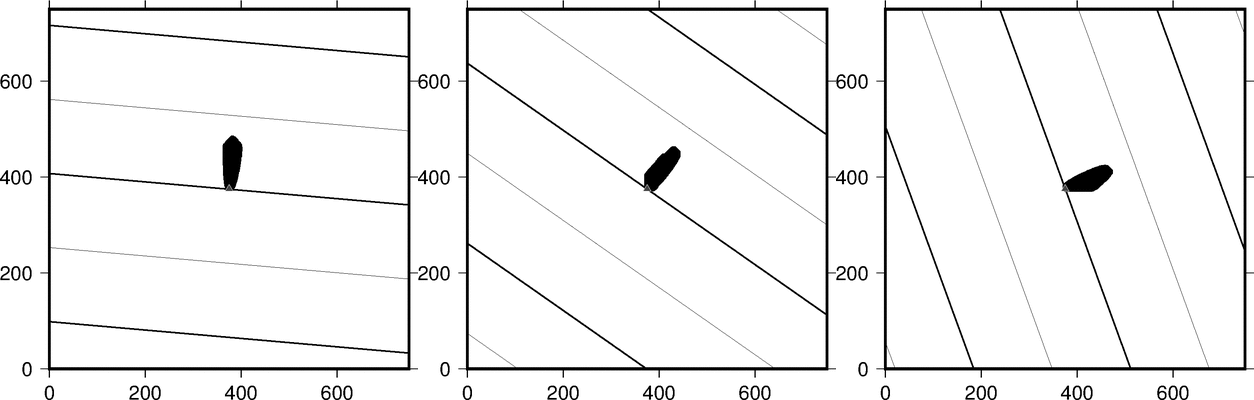
\includegraphics[width=\linewidth]{\FigPath/lava_C_4N_slope}
			\caption[Rotating slope test for the LavaPL algorithm]{Rotating slope test for algorithm \textbf{4/P/S} (LavaPL). Slope dip is 18$^{\circ}$, with dip-directions 0N, 30N, and 80N from left to right. The flow length and aspect ratio are similar and the flow direction is in the slope direction, so it passes Level 1 criteria.}
			\label{fig:slope}
		\end{figure}
		
		\subsubsection{Benchmark Parameters} The underlying DEM for this benchmark has a simple 18$^{\circ}$ slope, dipping to the North. The DEM has a spatial resolution of 1~m. The source cell is placed at the center of the DEM, is given a total volume of 1000~m$^3$, and is given a pulse volume of 1~m$^3$. When the simulation is finished, model output is used to determing the three flow characteristics used in this benchmark (length, orientation, and aspect ratio). The DEM is rotated 5$^{\circ}$ clockwise and the process is repeated 19 times until the flow is simulated on an East-facing slope.
		
		
		
		\subsubsection{Results}

		For all eight flow algorithms, flow length, aspect ratio, and orientation were calculated 19 times, corresponding to the 19 dip directions sampled between 0$^{\circ}$N and 90$^{\circ}$N. Variance for length and aspect ratio were calculated as the ratio of their standard deviations to their means. For instance, if mean runout length for the 18 flows is 100~m and the standard deviation of the 18 lengths is 2~m, the runout length variance is 2\%. The mean direction error is also calculated for the set of flows from each algorithm. These are reported in the table below.

			\begin{center}
				\textbf{DEM Rotation Results}
				
				\begin{tabular}{l c c c}
					\toprule
					Transition&Run-out&Aspect Ratio&Mean Direction\\
					Function&Variance&Variance&Error\\
					\midrule
					4/P/S &2.7\%&6.7\%&1.2$^{\circ}$\\
					8/P/S &4.4&12.2&0.9\\
					4/N/S &9.6&19.7&1.3\\
					8/N/S &3.9&7.5&0.6\\
					4/P/E &21.6&38.6&14.2\\
					8/P/E &7.2&13.8&5.4\\
					4/N/E &21.6&38.7&14.1\\
					8/N/E &7.2&13.8&5.5\\
			
					\bottomrule
				\end{tabular}
			\end{center}

			While with an ideal spreading algorithm, variances and direction error would be 0 under a rotating slope, every spreading algorithm tested performed differently as DEM direction changed. Following from the above pass-fail standards, five of the eight algorithms can be rejected. Algorithms 4/P/E and 4/N/E have high run-out length variance. Algorithms 4/N/S, 4/P/E and 4/N/E have large aspect-ratio variance. Algorithms 4/P/E, 8/P/E, 4/N/E, and 8/N/E all systematically deviate from running downslope by $>5^{\circ}$ on average. This implies that algorithms which share lavas equally from central cells to all lower neighboring cells perform worse than algorithms which share lavas proportional to slope.
			
			For the eight different transition functions tested, runout length varied between 60-160~m. The flow algorithm with the least flow length variance was the 4-connected, parent-child, slope-proportional strategy implemented in LavaPL. Algorithms 4/P/S (LavaPL), 8/P/S, and 8/N/S cannot be rejected because of any of the three standards set in this benchmark.

	\subsection{Level 2: Replication of flow morphologies on simple physical surfaces}
	
	The second benchmarking level is the first step in validating lava flow algorithms against realistic flow expectations. Instead of parameter space being arbitrarily defined, which was the case in Level 1, the defined parameter space informs tests at this level as to what the model output should be. As lava flows on a large scale are well described as Bingham fluids, simulations can be tested against analytical solutions or experimental observations of these fluids in simple conditions. For instance, a lava flow on a perfectly flat surface might be expected to create a circular areal extent \citep{griffiths2000dynamics}.
	
			Here I measure flow algorithm performance on a flat surface from a single vent source location. To measure the extent to which the simulated flow replicates a circle, the inundated area is compared to the area of a circle which circumscribes the flow exactly. This can be described as
			\begin{equation}
				Fit = \frac{A_{flow}}{\pi d_{max}^2}
			\end{equation}
			where $d_{max}$ is the farthest extent of the simulated flow from the vent. A perfect match to a circle would result in a $Fit=1$. With the same maximum distance from the vent (i.e. the distance from the center to a vertex) a perfect square would cover 64\% of the area of a circle, ergo $Fit=0.64$. An octagon would have a fit of 0.90. We consider a model to successfully pass this test if it produces a flow of $Fit>0.90$, or if the flow approximates a circle better than an octagon. The model unambiguously fails this test if if produces a flow of $Fit<0.64$, where a square better describes a circle than a flow generated from the model.

			\begin{center}
				\textbf{Circular Flow Test}
				
				\begin{tabular}{l l}
					\toprule
					Fit = 1.0 & Best Possible Score; perfectly circular.\\
					Fit $>$ 0.90 & Success; better than an octagon. \\
					Fit $<$ 0.64 & Failure; worse than a square.\\
					\bottomrule
				\end{tabular}
			\end{center}
		
		\begin{figure}[!h]
		\centering
		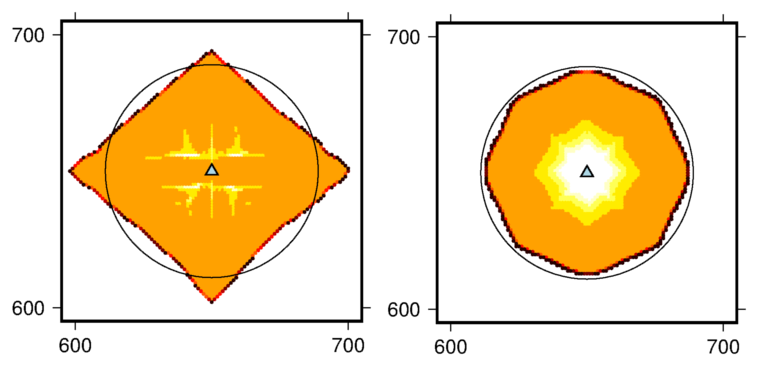
\includegraphics[width=\linewidth]{\FigPath/pancake}
		\caption[Fitness scores of different shaped flows on a flat surface]{Fitness scores of different shapes. From left to right: A circle has a perfect fit score of 1.00; an octagon has 0.90 times the area of a circumscribing circle; a square has a score of 0.64; Two flat surface tests for slope proportional spreading algorithms with parent rules. The flow second to the right is 4-connected (4/P/S) and has a score of 0.55, while the rightmost flow is 8-connected (8/P/S) with a score of 0.95. While the 4/P/S flow scores worse than a square, its 8-connected version passes the test as it scores better than an octagon.}
		\label{fig_pancake}
	\end{figure}
	
		\subsubsection{Benchmark Parameters} The DEM used in this benchmark is a horizontal plane (all grid locations have the same elevation) with a spatial resolution of 1~m. A single vent is located at the DEM center with a total volume of 1000~m$^3$, and a pulse volume of 1~m$^3$. When the simulation is finished, model output is used to find the inundated cell farthest from the vent ($d_{max}$). The total inundated area is divided by the area of a circle with radius $d_{max}$ to provide the Fit score.
		
		\subsubsection{Results}

		Five of the eight algorithms unambiguously passed the test of performing better than an octagon. In this test 8-connected algorithms outperformed 4-connected algorithms. Four algorithms unambiguously passed this test: 8/P/S, 8/N/S, 4/N/E, and 8/N/E.
		
		\begin{center}
			\textbf{Bingham Circle Results}\\
			\begin{tabular}{l c l}
				\toprule
				Algorithm&Circularity&\\
				\midrule
				4/P/S & 0.55 & Worse than a square.\\
				8/P/S & 0.95 & Better than an octagon.\\
				4/N/S & 0.55 & Worse than a square.\\
				8/N/S & 0.98 & Better than an octagon.\\
				4/P/E & 0.77 & Between a square and an octagon.\\
				8/P/E & 0.80 & Between a square and an octagon.\\
				4/N/E & 1.00 & Perfectly circular.\\
				8/N/E & 0.99 & Better than an octagon.\\
				
				\bottomrule
			\end{tabular}
		\end{center}
		
	\subsection{Level 3: Replication of real lava flows over complex topography}\label{sec_tolb_bench}
		The recent availability of global or near-global topographic datasets, such as SRTM or ASTER GDEM has enabled the direct observation of the underlying surface of even more recent lava flows. Flow algorithms can be validated against recent lava flows by simulating lava over these surfaces with parameters defined by the new lava flows. The 2012-3 Tolbachik lava flows will be used as a benchmark for the eight flow algorithms. As discussed above (Section \ref{sec_tolb_back}), the earliest lavas flowed from a fissure to the west. Before later stage flows began moving to the east, the volume of the lavas were 0.22~km$^3$. The modal thickness of the flow has been found to be 7.8~m and the areal extent was mapped with orthoimages \citep{kubanek2015lava}.

		For this example, two metrics which are commonly employed to validate lava flow simulators against real flows will be used: model sensitivity and a fitness metric called the ``Jaccard coefficient.'' An alternative bayesian approach to these metrics is discussed in Section \ref{sec:Bayesian}.  Model sensitivity is defined as
		\begin{equation}
			\text{Model~Sensitivity}=\frac{|Lava\cap Sim|}{|Lava|}
		\label{eq_sensitivity}
		\end{equation}
		where $|Lava\cap Sim|$ is the size of the interesection of the simulation and the true lava flow (the True Positives) and $|Lava|$ is the size of the lava flow. This gives a percentage of the true lava flow that the simulation correctly predicted. 
		
		The Jaccard coefficient, or fit, is defined as 
		\begin{equation}
			\text{Jaccard~Fit}=\frac{|Lava\cap Sim|}{|Lava\cup Sim|}
		\end{equation}
		where $|Lava\cup Sim|$ is the size of the union of the lava flow and a simulated flow. This gives a percentage of the total area covered by either the simulated flow or the true flow that is covered by both.
		
		Each flow algorithm is run using the following parameters. Flows are run over both 3-arcsecond SRTM topography (75 m grid resolution at 56$^{\circ}$N) and bistatic TanDEM-X topography processed by \citet{kubanek2015lava}. The pulse volume, the volume added to vent cells at each code loop (i.e. each instance of the PULSE module), is set at the product of the grid-cell area (5600 m$^2$ for the SRTM DEM and 225 m$^2$ for the TanDEM-X DEM) and the residual thickness (7.8~m). Both fitness metrics are calculated with the resulting model output, given as a list of inundated locations. ``Failure'' can be defined here as either metric falling below 50\% for the sake of example.
		
		\begin{center}
			\textbf{Tolbachik Validation Flow Parameters}\\
			\begin{tabular}{l l}
				\toprule
				Elevation Model & 75-m SRTM or 15-m TanDEM-X\\
				Residual Thickness & 7.8~m\\
				Pulse Volumes & 44200 m$^3$ (SRTM) or 1800 m$^3$ (TanDEM-X)\\
				\midrule
				Vent$_N$ Easting & 582800~m (UTM Zone 57)\\
				Vent$_N$ Northing & 6182100~m\\
				Vent$_N$ Total Volume & 4.63$\cdot10^7$~m$^3$\\
				\midrule
				Vent$_S$ Easting & 582475~m\\
				Vent$_S$ Northing & 6180700~m\\
				Vent$_S$ Total Volume & 1.737$\cdot10^8$~m$^3$\\
				\bottomrule
			\end{tabular}
		\end{center}
			
	\subsubsection{Results}
	
	\begin{figure}[!h]
			\centering
			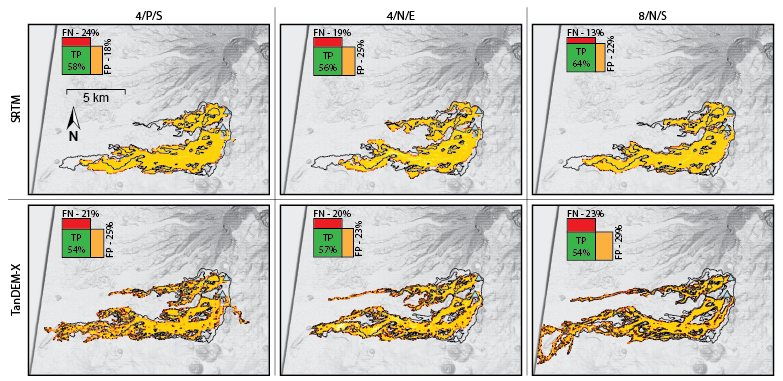
\includegraphics[width=\linewidth]{\FigPath/tolb_lvl3_examples_72dpi}
			\caption[Three transition function algorithms simulating the 2012-3 Tolbachik lava flows]{Three simulation algorithms (4/P/S, 4/N/E, and 8/N/S) applied to two elevation models (SRTM and TanDEM-X) to simulate the 2012-3 Tolbachik lava flows, outlined in black. Lava is emitted from two vent locations marked as blue triangles in the simulation. Diagrams showing the relative True Positives (green), False Positives (orange), and False Negatives (red) are illustrated in the top left of each simulation.}
			\label{fig:tolbachik}
		\end{figure}
	
	Three example algorithms are illustrated in Figure \ref{fig:tolbachik}. One primary observation is that all simulations had a longer run-out length on the finer TanDEM-X grid than on the coarser SRTM grid. Despite this, all flows took the correct major pathways taken by the true lava flow. A small diagram in the top left corner of each map in Figure \ref{fig:tolbachik} shows the true positives, false positives, and false negatives in each simulation. True positives are areas inundated by both flow and simulation, false positives are areas simulated as being inundated but are not mapped as such, and false negatives are areas hit by lava that the simulation failed to forecast. 
		
			The best algorithm and DEM pair were the 8/N/S algorithm over SRTM (top left of Figure \ref{fig:tolbachik}), while this same algorithm performed fairly poorly over TanDEM-X topography. For the SRTM simulation, this algorithm achieved a model sensitivity of 82.8\% and a Jaccard fitness score of 63.1\%. Graphically, sensitivity is calculated as the green area in the Figure \ref{fig:tolbachik} diagram divided by the green and red areas. The Jaccard fitness is the green area divided by the total area of the diagram. Because the Jaccard fitness statistic essentially expands the denomenator of model sensitivity, it will never be higher than model sensitivity.
			
			If success and failure are defined by having a fits of greater or less than 50\%, all models tested would pass for the SRTM DEM and about half would pass for the TanDEM-X DEM. All but one model (4/P/E) performed worse on the TanDEM-X DEM. The Jaccard fit and Sensitivity for all models are given below.
					
		\begin{center}
			\textbf{Tolbachik Flow Results}\\
			\begin{tabular}{l c c | c c}
				\toprule
				Transition&\multicolumn{2}{c}{\textbf{SRTM DEM}}&\multicolumn{2}{c}{\textbf{TanDEM-X DEM}}\\
				Function& Jaccard & Sensitivity& Jaccard & Sensitivity\\
				\midrule
				4/P/S & 56.7\%& 76.4\%& 53.0\%& 72.4\% \\
				8/P/S & 61.1  & 80.8  & 46.8  & 67.2   \\
				4/N/S & 57.2  & 77.5  & 44.0  & 64.0   \\
				8/N/S & 63.1  & 82.8  & 46.7  & 67.4   \\
				4/P/E & 51.2  & 71.5  & 54.2  & 73.4   \\
				8/P/E & 58.8  & 78.2  & 56.3  & 76.0   \\
				4/N/E & 54.5  & 74.5  & 55.7  & 73.7   \\
				8/N/E & 59.6  & 78.8  & 56.2  & 75.3   \\
				
				\bottomrule
			\end{tabular}
		\end{center}


%%%%%%%%%%%%%%%%%%%%%%%%%%%%%%%%%%%%%%%%%%%%%%%%
%BAYESIAN APPROACH
%%%%%%%%%%%%%%%%%%%%%%%%%%%%%%%%%%%%%%%%%%%%%%%%
%%%%%%%%%%%%%%%%%%%%%%%%%%%%%%%%%%%%%%%%%%%%%%%%
%%%%%%%%%%%%%%%%%%%%%%%%%%%%%%%%%%%%%%%%%%%%%%%%
\section{Bayesian Applications for Lava Flow Models}\label{sec:Bayesian}
	The final step \citet{bayarri2007framework} give for validating computer models is ``feeding [observations and results] back to revise the model.''
	
	The use of computer models to forecast hazards is a fundamentally Bayesian strategy: there is an initial concern due to hazards and computer models help us inform, constrain, and update this concern. Using Bayesian statistics can therefore be an improvement in testing lava flow models, over the two commonly used fitness tests, model sensitivity and the Jaccard index, because of their more direct application to informing perceived risk. 
	
	Three tools will be used in this section: A posterior probability, a ``negative'' posterior probability, and a Bayes factor. Bayes theorem connects a phenomenon $A$ to observations $B$ through the function
	\begin{equation}
		\text{Pr}(A|B)=\frac{\text{Pr}(B|A)\text{Pr}(A)}{\text{Pr}(B)}\label{eq_bayes}
	\end{equation}
	where $\text{Pr}(A)$ is the general probability of $A$ occuring, $\text{Pr}(B)$ is the probability of $B$ being observed, and $\text{Pr}(B|A)$ is the conditional probability of $B$ given the occurence of $A$. $\text{Pr}(B|A)$ is also known as model sensitivity, which is a common fitness statistic and was discussed in Section \ref{sec_tolb_bench}
	
	The left side of Equation \ref{eq_bayes}, $\text{Pr}(A|B)$, is the Posterior probability of $A$ and can be stated as ``the probability that lava will inundate a location if the model forecasted inundation at that location.'' A second posterior, which I call the negative posterior, is $\text{Pr}(\neg A|\neg B)$ and is the obverse of $\text{Pr}(A|B)$. This negative posterior relates not being inundated by lava at a given location to a safe outcome forecasted by a simulation and can be calculated by modifying Equation \ref{eq_bayes} and substituting $A$ for $Lava$ (the lava flow) and $B$ for $Sim$ (the simulation), resulting in the formula
	\begin{equation}
		\text{Pr}(\neg Lava|\neg Sim)=\frac{\text{Pr}(\neg Sim|\neg Lava)\text{Pr}(\neg Lava)}{\text{Pr}(\neg Sim)}
	\end{equation}
	where the $\neg$ symbol indicates the event or observation not happening, and $\text{Pr}(\neg Sim|\neg Lava)$ is model specificity.
	
	The negative posterior is important in hazard forecasting as it is in some sense a probability of safety. The more common posterior $\text{Pr}(A|B)$ (or $\text{Pr}(Lava|Sim)$) does not contain information about areas that the simulation does not inundate; while it can support the hypothesis that lava will hit a location given a simulated hit, it cannot estimate one's relative risk if the simulation forecasts a safe outcome. The negative posterior $\text{Pr}(\neg Lava|\neg Sim)$ does just this, and informs a user whether to rely on a safe outcome from a simulation. If, for example, the posterior probability $\text{Pr}(Lava|Sim)$ is high while the negative posterior probability $\text{Pr}(\neg Lava|\neg Sim)$ is low for a given lava flow simulator, areas that are evacuated due to the simulation outcome will be evacuated for good reason, but many areas will likely be inundated that were not evacuated due to the simulation outcome. This is why it is important to estimate and ultimately try to improve both posterior metrics.
	
	Bayes factors provide a tool to test the relative likelihood of a hypothesis against another. \citet{aspinall2003evidence} introduced this tool to volcano hazard forecasting by testing whether the onset of particular seismic events before the 1993 Galeras catastrophe was a significant indicator of the eruption or not. A Bayes Factor (BF) relating two models is given by \citet{jeffreys1998theory} as
	\begin{equation}
		\text{BF} = \frac{\text{Pr}(\text{Data}|\text{Model~1})}{\text{Pr}(\text{Data}|\text{Model~2})}
		\label{eq_BF}
	\end{equation}
	In the example of Galeras, the ``data'' are the seismic events, Model 1 is ``imminent explosion,'' and Model 2 is ``not imminent explosion'' \citep{aspinall2003evidence}. Below, I will apply this with the data being the probability of simulated inundation and the models ``lava inundation'' and ``not lava inundation.'' \citet{jeffreys1998theory} provided a log-scale interpretation to the value of BF in Equation \ref{eq_BF}, given in the Table \ref{tab_BFinterps}.
	
	\begin{table}[h]
		\centering
		\caption{Bayes Factor Interpretations (modified from \citet{aspinall2003evidence})}
		\begin{tabular}{l l}
			\toprule
			BF Value & Description\\
			\midrule
			$BF>10^2$ & Evidence for Model 1 is Decisive.\\
			$10^{1.5}<BF<10^2$ & Evidence for Model 1 is Very Strong.\\
			$10^{1}<BF<10^{1.5}$ & Evidence for Model 1 is Strong.\\
			$10^{0.5}<BF<10^{1}$ & Evidence for Model 1 is Substantial.\\
			$10^{0}<BF<10^{0.5}$ & Evidence for Model 1 is just worth a mention.\\\\
			$10^{-0.5}<BF<10^{0}$ & Evidence for Model 2 is just worth a mention.\\
			$10^{-1}<BF<10^{-0.5}$ & Evidence for Model 2 is Substantial.\\
			$10^{-1.5}<BF<10^{-1}$ & Evidence for Model 2 is Strong.\\
			$10^{-2}<BF<10^{-1.5}$ & Evidence for Model 2 is Very Strong.\\
			$BF<10^{-2}$ & Evidence for Model 2 is Decisive.\\
			\bottomrule
		\end{tabular}
		\label{tab_BFinterps}
	\end{table}
	
		In the same manner as the final validation level, the statistics discussed above will be calculated based on the areal extent of flows and simulations. The probability of the lava flow inundating an area $N$ can be given as
		\begin{equation}
			\text{Pr}(A)=\frac{|Lava|}{|N|}\label{eq_PA}
		\end{equation}
		where $|Lava|$ is the areal size of the flow (i.e. literally the number of DEM grid cells the lava inundates) and $|N|$ is the size of the area of interest, or the potential hazard area. The probability of the simulation is similarly found to be
		\begin{equation}
			\text{Pr}(Sim)=\frac{|Sim|}{|N|}.\label{eq_PB}
		\end{equation}
		By substituting these definitions and model sensitivity (Equation \ref{eq_sensitivity}, $|Lava \cap Sim|/|Lava|$) in Equation \ref{eq_bayes}, the posterior probability of lava flow inundation, given a simulation that forecasts inundation can be recast as
		\begin{align}
		\text{Pr}(Lava|Sim)&=\frac{\frac{|Lava\cap Sim|}{|Lava|}\frac{|Lava|}{|N|}}{\frac{|Sim|}{|N|}}~\text{,~or~simplified,}\label{eq_unsimplepost}\\
		&=\frac{|Lava\cap Sim|}{|Sim|}.\label{eq_simplepost}
		\end{align}
		where $|Lava\cap Sim|$ is the size of the intersection of the lava flow and simulated flow (again, the number of DEM grid cells). Note that this posterior probability is independent of the potential hazard area.
		
		The negative posterior can be stated in terms of the sizes of the lava flow and simulated flow as well.
		\begin{equation}
			\text{Pr}(\neg Lava|\neg Sim)=\frac{|\neg Lava\cap \neg Sim|}{|\neg Sim|}\label{eq_simplenegpost}
		\end{equation}
		Calculating the size or number of grid cells of $\neg Lava$ or $\neg Sim$ is fundamentally dependent on the potential hazard area, as $|\neg Lava|$ is defined as
		\begin{equation}
			|\neg Lava| = |N| - |Lava|.
		\end{equation}
		Because of this, we must define the size of the potential hazard area $N$ ($|N|$).	
	
	\paragraph{Potential Hazard Area} There are multiple strategies to estimating an \textit{a priori} hazard area. \citet{kauahikaua1995applications} for instance identified catchments or ``lava sheds'' in which a volcanic vent was erupting, and identified these lava sheds as the hazard area. \citet{kilburn2000lava} provided a theoretical maximum distance that a lava flow can travel given the mass flux of magma erupting at the vent location. A combination of these two would provide an objective hazard area defined as the area within the ``Kilburn distance'' that is topographically below the volcanic vent. The theoretical maximum distance, or hazard radius, given by \citet{kilburn2000lava} is
		\begin{equation}
		R_{max}=\sqrt{\frac{3\epsilon SQ}{\rho g\kappa}}
		\label{eq_kilburn}
		\end{equation}
	where $\epsilon$ is an empirical value related to the amount of extension of lava crust allowed before it fails (10$^{-3}$), $S$ is the tensile strength of this crust (10$^7$~Pa), $\rho$ is the lava crust density (2200~kg~m$^{-3}$), $g$ is gravitational acceleration, $\kappa$ is the bulk thermal diffusivity ($4\times 10^{-7}$~m$^{2}$~s$^{-1}$) and $Q$ is the mean volumetric flow rate from the vent. From this, the hazard radius for the Tolbachik 2012-3 flow is calculated to be 39~km, given a magma flux of 440~m$^3$~s from the vent as was estimated early in the eruption \citep{belousov2015overview}. The total area within this radius that is also below the vent-plus-modal-flow-thickness elevation is 1,415~km$^2$. Note that the mapped flow area of 26~km$^2$ only covers 1.9\% of this defined hazard area (i.e. $\text{Pr}(Lava) = 0.019$).
	
		\begin{figure}
			\centering
			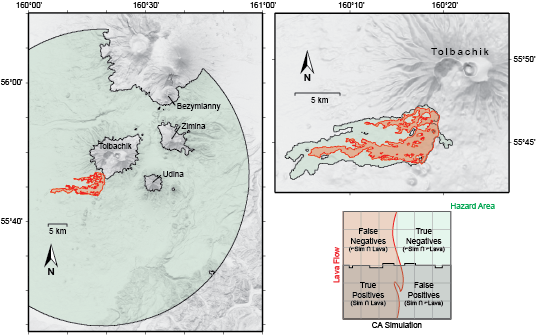
\includegraphics[width=0.7\linewidth]{\FigPath/hazard_areas_72dpi}
			\caption[Potential hazard areas of the 2012-3 Tolbachik Flows]{Potential hazard areas of the 2012-3 Tolbachik Flows in light green, defined by a maximum flow radius (left, Equation \ref{eq_kilburn}) and the total areal coverage of 100,000 random flow simulations (top-right, Section \ref{sec_MC}). The mapped lava flow is red. The chart to the bottom right shows four regions defined by the presence or absense of lava and simulated lava across a map grid.}
			\label{fig_hazardarea}
		\end{figure}
	
	A second strategy would be to run many lava flow models from the known vent location(s) while varying input parameters. This would give a range of flows and the true flow might be completely contained within the region given by this range of simulations. Below, a Monte Carlo (MC) method will be used to simulate a large range of flows. If we define a potential hazard area as any location inundated by at least one simulated flow in this MC approach, the hazard area would be 72~km$^2$. As the mapped flow area from the Tolbachik eruption is 39\% of this area, it would be more practical to use this as the \textit{a priori} hazard area because it more reasonably reflects the potential inundation area. Both the Kilburn-Kauahikaua method and this MC method are illustrated in Figure \ref{fig_hazardarea}.				
	
	\paragraph{Review of Validation Level 3} Instead of using model sensitivity and the Jaccard index as benchmarks for the various lava flow models, now the two posteriors will be used. The potential hazard area is defined as the distribution of MC simulations (72~km$^2$). To give an example calculation, $\text{Pr}(Lava|Sim)$ is found with Equation \ref{eq_simplepost} by dividing true positives (green boxes in \ref{fig:tolbachik}) by the simulation area (green and red boxes). The negative posterior, $\text{Pr}(\neg Lava|\neg Sim)$, is found by diving true negatives (blue area, in bottom right diagram of Figure \ref{fig_hazardarea}), by the area not simulated (top half of bottom right diagram of Figure \ref{fig_hazardarea}).
	
		\begin{center}
		\textbf{Traditional Fit Metrics and Bayesian Posterior Functions}\\
		\begin{tabular}{l c c c c}
			\toprule
			Transition&\multicolumn{4}{c}{\textbf{Results of simulations over SRTM DEM}}\\
			Function& Jaccard & Sensitivity & $\text{Pr}(Lava|Sim)$ & $\text{Pr}(\neg Lava|\neg Sim)$\\
			\midrule
			4/P/S & 56.7\%& 76.4\%& 70.4\%& 84.5\% \\
			8/P/S & 61.1  & 80.8  & 73.2  & 87.3   \\
			4/N/S & 57.2  & 77.5  & 70.3  & 85.1   \\
			8/N/S & 63.1  & 82.8  & 74.4  & 88.5   \\
			4/P/E & 51.2  & 71.5  & 66.0  & 81.4   \\
			8/P/E & 58.8  & 78.2  & 72.0  & 85.7   \\
			4/N/E & 54.5  & 74.5  & 68.7  & 83.3   \\
			8/N/E & 59.6  & 78.8  & 72.8  & 86.2   \\
			
			\bottomrule
		\end{tabular}
	\end{center}
	
	For the rest of this section, the 8/N/S (the 8-connected, no parent-child relationships, with slope-proportional spreading) algorithm will be used. This is preferred because it out-performed other algorithms over the SRTM DEM. By applying this model to the Tolbachik lava flows, Bayesian methods will be used to improve the ``Pulse Volume'' parameter and will later be used to constrain model uncertainty at Tolbachik.
	
	\subsection{Improving model performance on one model parameter}\label{sec_bayespulse}
	In the Tolbachik benchmark tests given as examples of comparing simulation algorithms against real lava flows (Section \ref {sec_tolb_bench}), all but one algorithm performed worse on the TanDEM-X derived elevation model. This was in part due to large run-out distances in the simulations (e.g. bottom right of Figure \ref{fig:tolbachik}), which considerably increased simulation false positives. The large run-out distances might be due to the pulse volume, the volume of lava given to source cells at each code loop in MOLASSES, being poorly chosen. Here, the Bayesian statistics defined above will be used to compare different pulse volumes and identify an optimal pulse volume. 
		
		An optimal pulse volume will ideally produce a flow simulation with the highest posterior and negative posterior value. Pulse volumes with high associated posterior values will produce simulations where areas simulated as inundated by lava will have a high likelihood of actually being inundated by lava. Pulse volumes with high associated negative posterior values will produce simulations where areas simulated to not be inundated will hava a high likelihood of actually not being inundated.
		
		\subsubsection{Model Execution} 
		To populate $Sim$, I have run the MOLASSES lava flow code using TanDEM-X derived parameters listed in Table \ref{tab_parameters_pulsebayes}. All variables are fixed except the pulse volume parameter, which is the amount of lava delivered to source cells in the Cellular Automata grid of MOLASSES. The lowest pulse volume, 1755 m$^3$ per pulse, is approximately the product of the TanDEM-X DEM grid cell size (225~m$^2$) and the residual flow thickness (7.8~m). The other 15 pulse volumes are multiples of this volume (i.e. they are 1.5 to 8.5$\times$ 1775 m$^3$).
		
		\begin{table}[h!]
		\centering
			\caption{MOLASSES Flow Parameters}
			\begin{tabular}{l l}
				\toprule
				Elevation Model & 15-m bistatic TanDEM-X, 11 Nov 2015\\
				Modal Thickness & 7.8~m\\
				Pulse Volumes & 16 equally separated volumes, [1755,14917] m$^3$\\
				\midrule
				Vent$_N$ Easting & 582800~m (UTM Zone 57)\\
				Vent$_N$ Northing & 6182100~m\\
				Vent$_N$ Total Volume & 4.63$\cdot10^7$~m$^3$\\
				\midrule
				Vent$_S$ Easting & 582475~m\\
				Vent$_S$ Northing & 6180700~m\\
				Vent$_S$ Total Volume & 1.737$\cdot10^8$~m$^3$\\
				\bottomrule
			\end{tabular}
			\label{tab_parameters_pulsebayes}
		\end{table}
		

		Model output is compared to a list of x,y locations in the Tolbachik area that have been inundated or not. This location list is stored in a raster with the same projection and extent as the elevation model used in MOLASSES. ASCII locations output by MOLASSES are also listed in the same projection within the same extent as the elevation model. This enables direct comparison between the Model information (i.e. $Sim$) and the mapped lava flow (i.e. $Lava$). True Positives, False Positives, and False Negatives are reported as cell counts (number of grid locations where $Lava$ and $Sim$ agree or not). Three examples of these simulations are mapped in Figure \ref{fig:pulse_map}.

		\begin{figure}
		\centering
		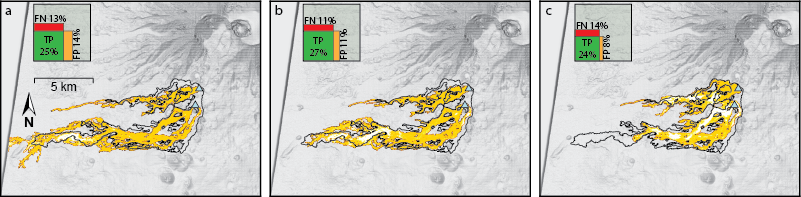
\includegraphics[width=\linewidth]{\FigPath/pulse_examples_72dpi}
		\caption[MOLASSES Simulations with different Pulse Volume parameter values of the 2012-3 Tolbachik Lava Flows]{MOLASSES Simulations of the 2012-3 Tolbachik Lava Flows. Vents are shown as blue triangles and the mapped flow is outlined in black. a) Pulse Volume = 1755 m$^3$, the simulation far exceeds the true runout distance; b) Pulse Volume = 4387 m$^3$, this simulation performs best under the negative posterior $\text{Pr}(\neg Lava|\neg Sim)$ test; c) Pulse Volume = 14040 m$^3$, this simulation performs best under the posterior $\text{Pr}(Lava|Sim)$ test, but does not have a runout length similar to the mapped flow.}
		\label{fig:pulse_map}
		\end{figure}

		\subsubsection{Results}
		
		Three example simulations are shown in Figure \ref{fig:pulse_map} using simulation parameters from Table \ref{tab_parameters_pulsebayes} and different pulse volume values. With increased pulse volume, simulated run-out distance is shorter. This is because the MOLASSES code ends once all volume is delivered to the vents and the DISTRIBUTE module has run once more. In other words, if the pulse volume is doubled, the number of times the PULSE and DISTRIBUTE modules will be run will be halved, as the total volume will be delivered to the vents in half the code loops (see Figure \ref{fig_flowchart}). By running DISTRIBUTE fewer times, cells have fewer opportunities to advect lava downslope.

		The posterior statistical measure is the fundamental tool of Bayesian statistics, and quantifying it enables an update of belief in risk of lava inundation. A perfect posterior value would mean that if the model simulates lava inundating a location, lava will certainly inundate that location. The posterior is calculated for simulated lava flows of different Pulse Volumes and is graphed in Figure \ref{fig_lavaGsim}. From this, it can be seen that the highest pulse volumes, which coincidentally form the shortest flow simulations, perform best with this test, with the best fit having a pulse volume of 14040~m$^3$ per algorithm loop (Figure \ref{fig:pulse_map},c). A local maximum does exist in the low pulse volumes at 4387~m$^3$ per loop.


		\begin{figure}[h!]
			\centering
			\begin{gnuplot}[terminal=latex, terminaloptions=rotate]
				unset key
				set size 0.7,0.7
				set format xy "$%g$"
				set xlabel "Pulse Volume (m$^3$)" rotate by 90
				set ylabel "Pr$(Lava|Sim)$"
				set ytics 0.05
				set xtics 4000
				plot "results_bayes.dat" using 1:2 with linespoints lt 4 pt 7
			\end{gnuplot}
			\caption{Posterior $\text{Pr}(Lava|Sim)$ for MOLASSES flows with differing Pulse Volumes.}
			\label{fig_lavaGsim}
		\end{figure}
		
		The negative posterior $\text{Pr}(\neg Lava|\neg Sim)$, is the percentage of non-inundated area in the simulation that is also not inundated in real life. A perfect negative posterior would indicate that, if a model does not simulate a hit for a location, lava will certainly not inundate that location. The negative posteriors of simulations with different pulse values are shown in Figure \ref{fig_neglavaGsim}. Unlike the previous posterior analyzed, the best performing flows have smaller pulse volumes and the best performing volume is 4387~m$^3$ per model pulse loop (Figure \ref{fig:pulse_map},b).

		\begin{figure}[h!]
			\centering
			\begin{gnuplot}[terminal=latex, terminaloptions=rotate]
				unset key
				set size 0.7,0.7
				set format xy "$%g$"
				set xlabel "Pulse Volume (m$^3$)" rotate by 90
				set ylabel "Pr(not $Lava|$not $Sim)$"
				set ytics 0.01
				set xtics 4000
				plot "results_bayes.dat" using 1:3 with linespoints lt 4 pt 7
			\end{gnuplot}
			\caption{Negative posterior $\text{Pr}(\neg Lava|\neg Sim)$ for MOLASSES flows with differing Pulse Volumes.}
			\label{fig_neglavaGsim}
		\end{figure}
	
	\subsection{Incorporating Model Uncertainty with a Monte Carlo method}\label{sec_MC}
		Model uncertainty is a result of input parameter uncertainty, such as uncertainty in the underlying DEM. This can be distinguished from model error, which might be defined as the difference between the true lava flow and a simulation carried out with perfect input parameters, and is created by the inherent deviations between a computer model and real life processes. Because there is parameter uncertainty, it is essential to quantify the range of model solutions given the likely range of each parameter.
		
		In this example, elevation uncertainty will be examined. Elevation uncertainty is an element in the MOLASSES module \textbf{INITFLOW}, where each grid cell elevation can be defined randomly before the lava flow simulation begins. The user can add an elevation uncertainty, in meters, to the configuration file. If this value is provided, each grid cell will receive a new elevation value randomly selected from a normal distribution whose mean is the DEM elevation and the standard deviation is the uncertainty value.
		
		\begin{table}[h!]
		\centering
			\caption{Monte Carlo MOLASSES Flow Parameters}
			\begin{tabular}{l l}
				\toprule
				Elevation Model & 75-m SRTM\\
				Elevation Uncertainty, $1\sigma$ & 3~m\\
				Residual Thickness & 7.8~m\\
				Pulse Volume & 44200 m$^3$\\
				\midrule
				Vent$_N$ Easting & 582800~m (UTM Zone 57)\\
				Vent$_N$ Northing & 6182100~m\\
				Vent$_N$ Total Volume & 4.63$\cdot10^7$~m$^3$\\
				\midrule
				Vent$_S$ Easting & 582475~m\\
				Vent$_S$ Northing & 6180700~m\\
				Vent$_S$ Total Volume & 1.737$\cdot10^8$~m$^3$\\
				\bottomrule
			\end{tabular}
			\label{tab_parameters_MC}
		\end{table}
		
		%Map of the MC flows
		\begin{figure}
			\centering
			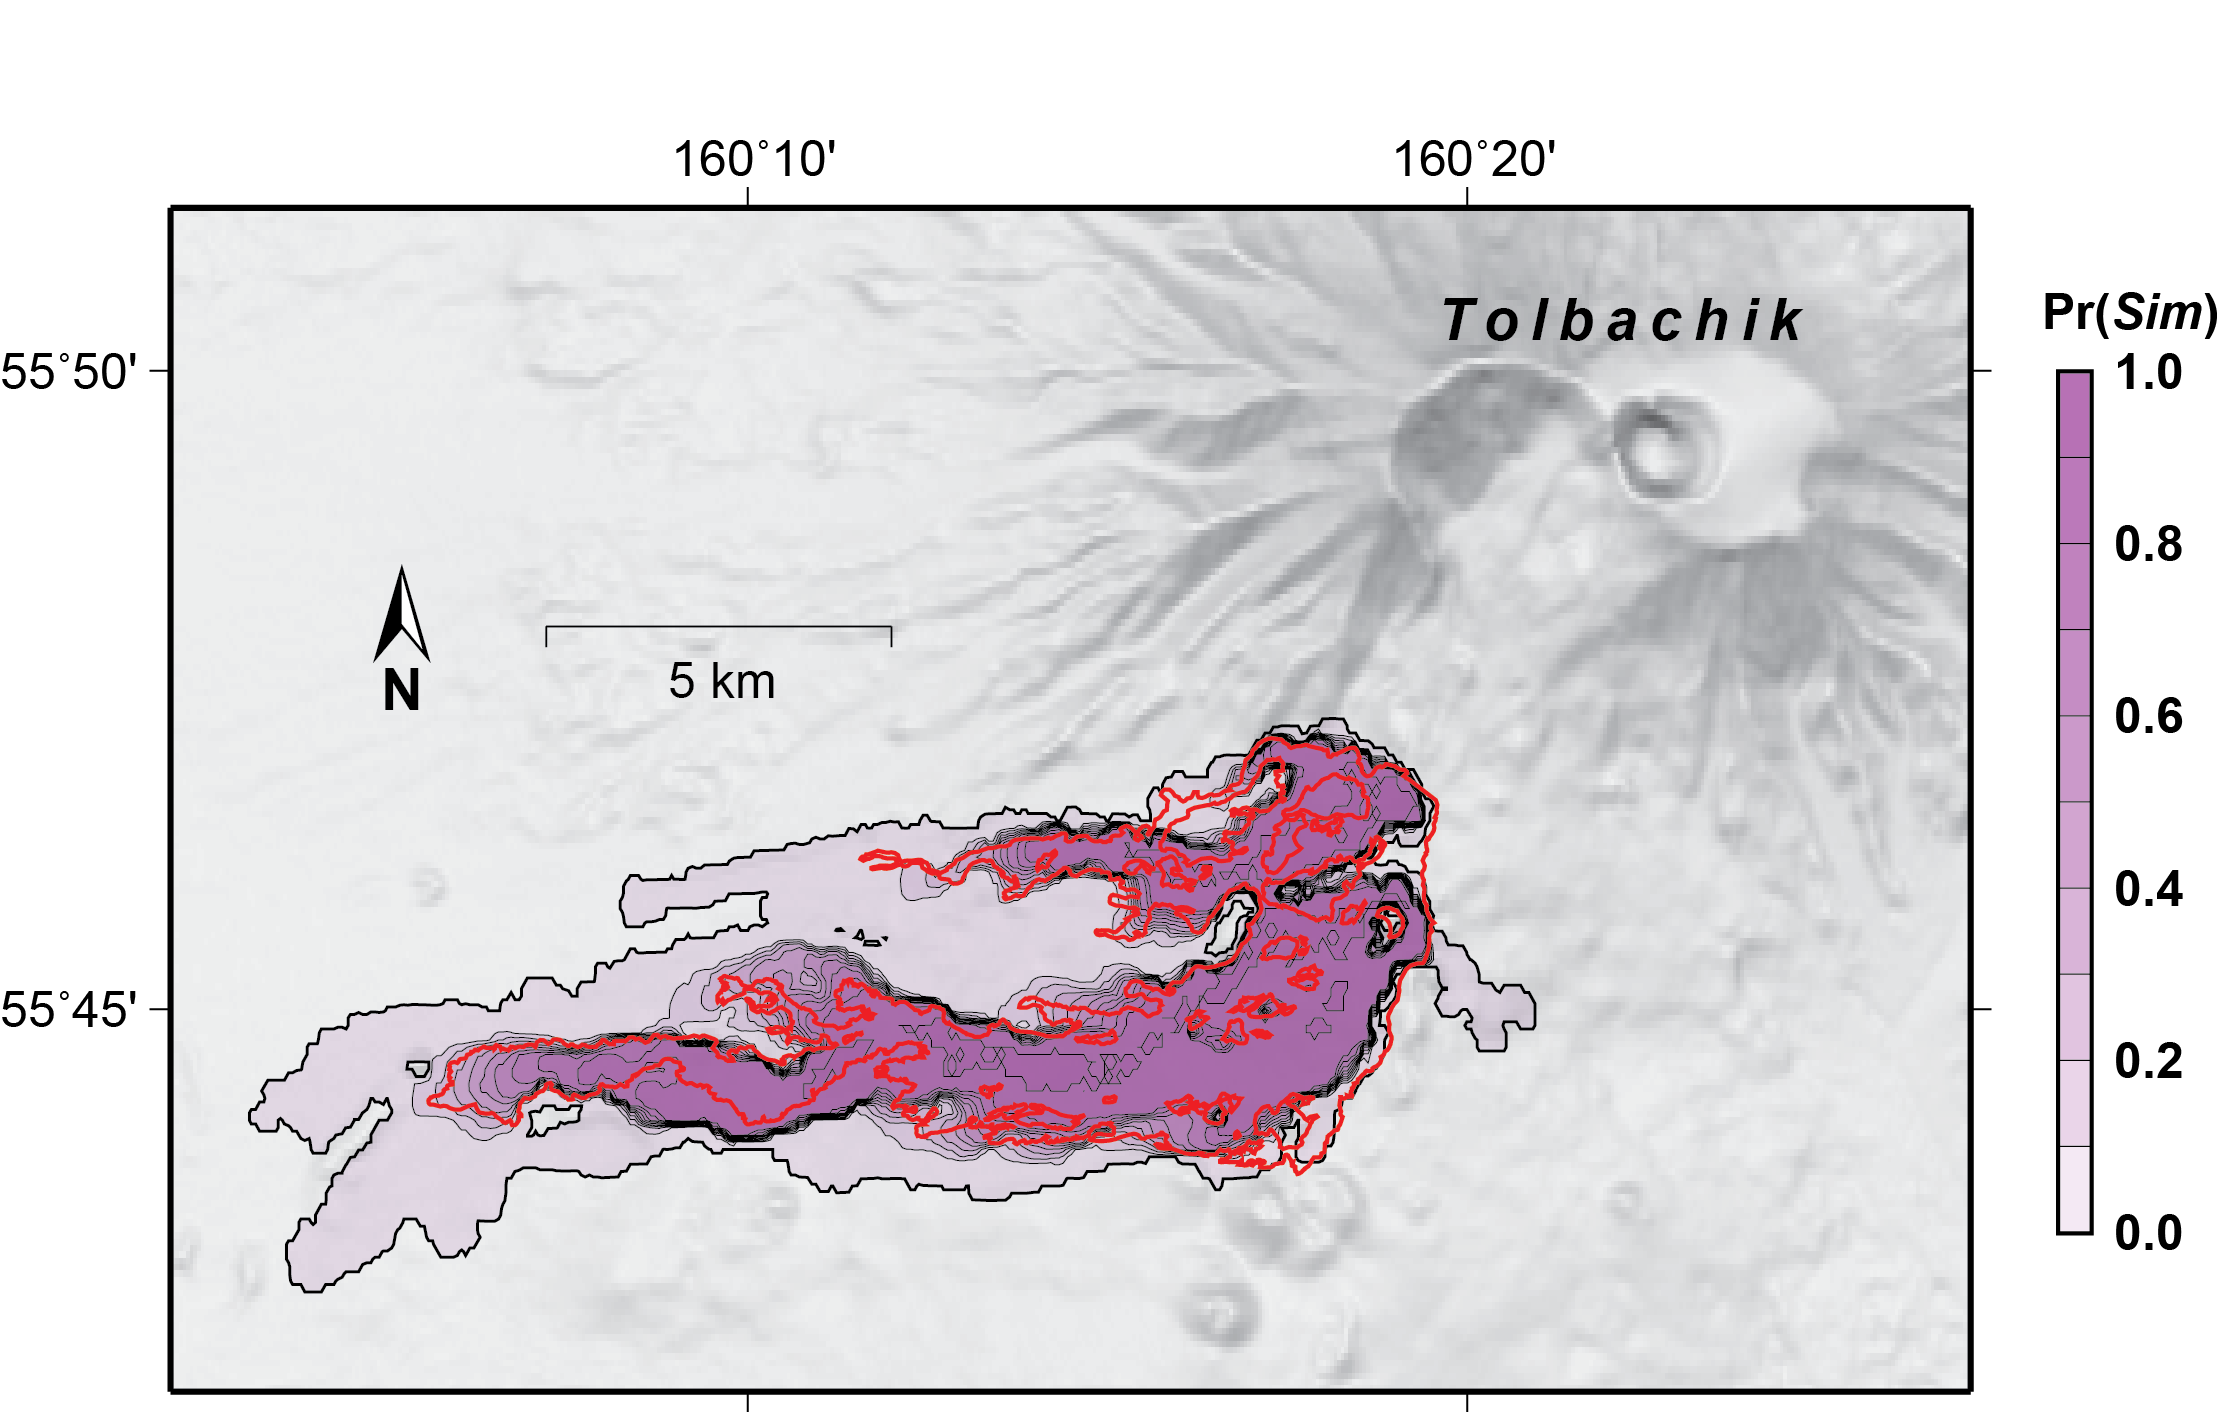
\includegraphics[width=0.7\linewidth]{\FigPath/MC_probmap_300dpi}
			\caption[Map of Monte Carlo simulations of the 2012-3 Tolbachik lava flows]{Cumulative distribution of 100,000 simulated lava flows over SRTM topography with 3~m elevation uncertainty. The red outline is the mapped flow extent of the 2012-3 Tolbachik flow. Darker purple areas represent more simulation hits (i.e. higher $\text{Pr}(Sim)$).}
			\label{fig_MC_map}
		\end{figure}
		
		The Monte Carlo method runs MOLASSES 100,000 times over a 75-m SRTM DEM. Vertical uncertainty of this data is estimated by \citet{rodriguez2006global} for Eurasia to be 6.2~m at a 90\% confidence level and is shown to be randomly distributed. With this result, elevation uncertainty in the MOLASSES model is given a value of $1\sigma=3$~m. Other input parameters remain unchanged from the benchmark exercise above; MOLASSES flow parameters for the Monte Carlo model are listed in Table \ref{tab_parameters_MC}. The combined 100,000 simulations are mapped in Figure \ref{fig_MC_map} where flow color indicates the number of flows that impacted each location.
		

				
		\subsubsection{Bayesian distribution of MC results}
			The reliability of a model can be better understood by showing the distribution of model performance given model uncertainty, as opposed to treating model parameters, and thus model output, as completely certain.  Figure \ref{fig:MC_dist} shows the distribution of the posterior and the negative posterior scores. Each dot in the main chart of Figure \ref{fig:MC_dist} represents a single flow simulation over a partially randomly generated DEM. The clustering of these points shows a positive correlation between the two posterior metrics, and both metrics are not normally distributed as shown on the histograms on either side of the main chart of Figure \ref{fig:MC_dist}. The flow simulation assuming no elevation uncertainty (shown in the top right corner of Figure \ref{fig:tolbachik}) fits the mapped flow better than the median value of both posteriors in the distribution, though it still lays within the MC distribution.
			
		%Graph of the performances
		\begin{figure}[h!]
			\centering
			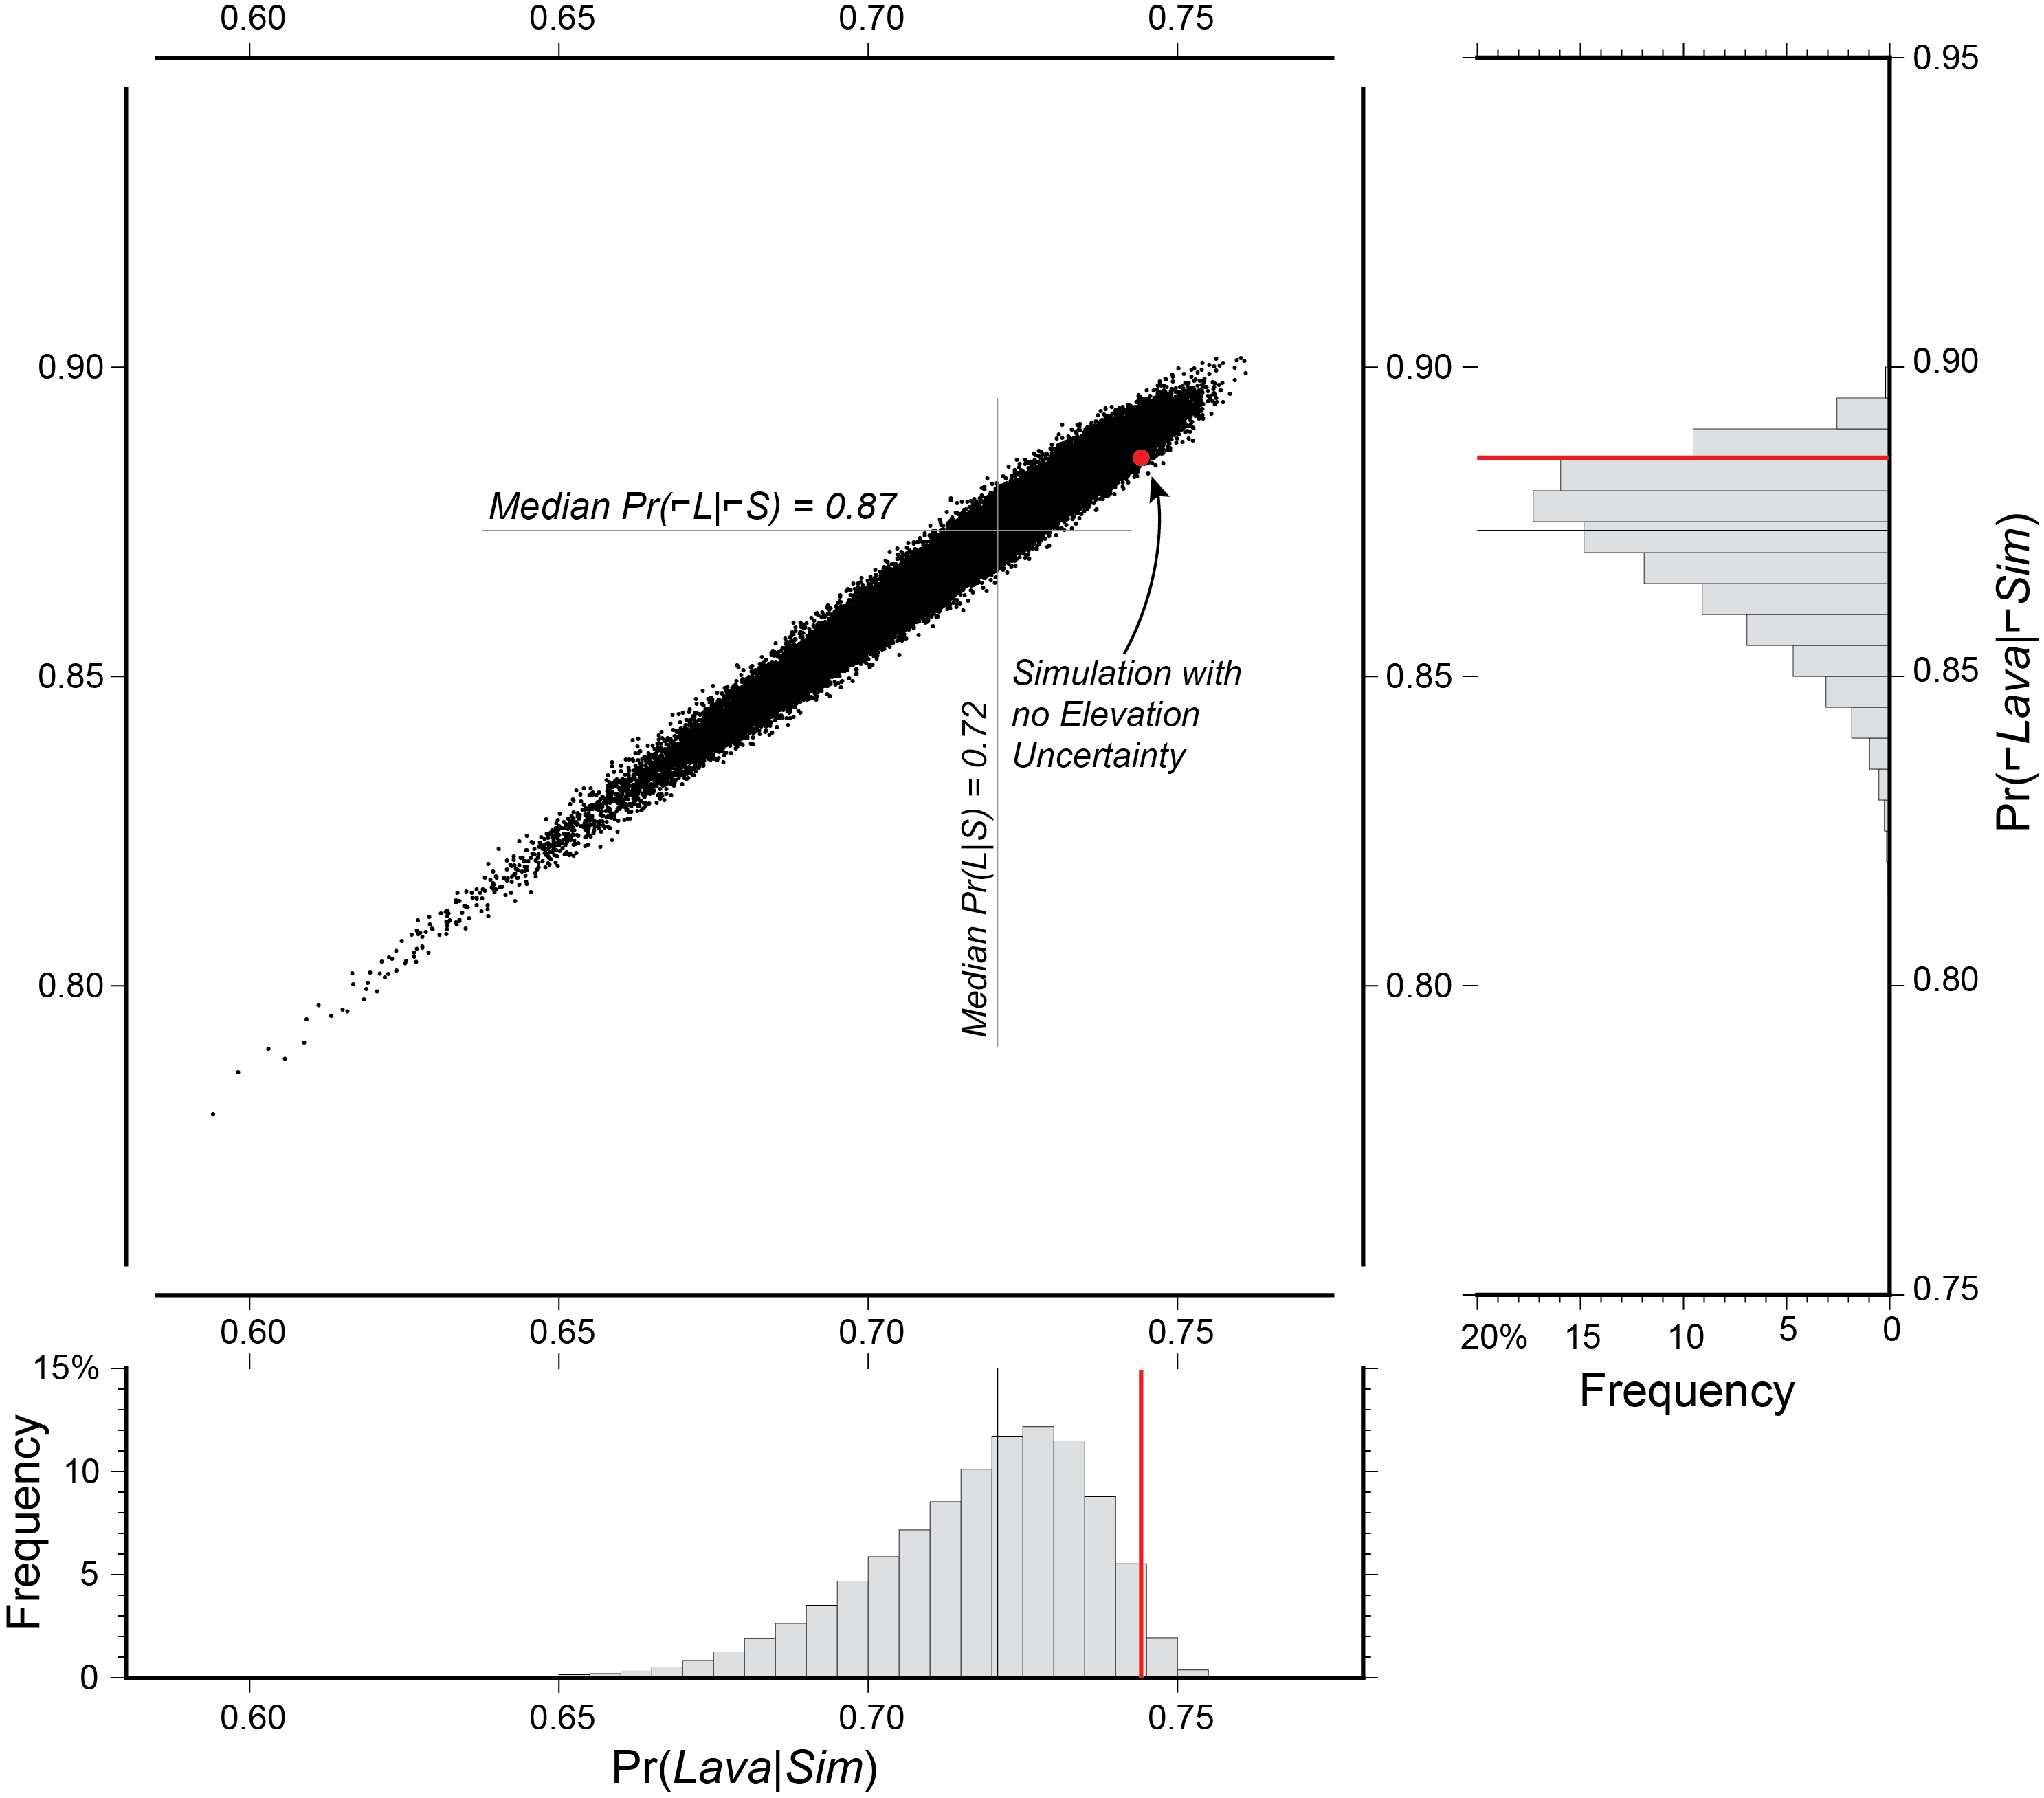
\includegraphics[width=0.7\linewidth]{\FigPath/MC_posteriors_300dpi}
			\caption[Fitness statistic distribution of Monte Carlo simulations of the 2012-3 Tolbachik lava flows]{Fitness statistic distribution between for 100,000 simulations of the 2012-3 Tolbachik Lava Flows, over SRTM topography with 3~m standard elevation uncertainty. Each point represents the posterior probabilities of inundation/non-inundation for one simulation. Red lines are the fitness values of a simulated flow over SRTM data assuming 0~m elevation uncertainty (top right corner of Figure \ref{fig:tolbachik}). Black lines are placed at the median values of each posterior probability.}
			\label{fig:MC_dist}
		\end{figure}
			
			If the elevation model used were perfect, the posterior values would be a single number ($\text{Pr}(Lava|Sim)=74.4$\% and $\text{Pr}(\neg Lava|\neg Sim)=88.5$\%). However, because elevation values have inherent uncertainty, model fitness, as defined by the posterior values, can be given as a range. Including elevation uncertainty, the $\text{Pr}(Lava|Sim)$ fitness has a range of 59-76\% and the $\text{Pr}(\neg Lava|\neg Sim)$ has a range of 77-91\%.


		\subsubsection{Estimating inundation risk from the simulated frequency of inundation}
		Figure \ref{fig_MC_map} shows a map view of the probability of inundation from the 100,000 MC simulations. Generally, areas within the mapped flow appear to be inundated by more simulations than outside the mapped flow. But can the probability of simulation inundation, $\text{Pr}(Sim)$, be used in a more formal way to judge the probability of lava inundation? In this section, the Tolbachik region map will be split into sub-regions based on $\text{Pr}(Sim)$, and the probabilities of inundation and not inundation will be compared.
		
		Three example sub-regions are shown in Figure \ref{fig_MCsubregions}. These sub-regions are defined as the area where $\text{Pr}(Sim)$ falls between a 10\% range. For instance, the top sub-region in Figure \ref{fig_MCsubregions} shows all locations that were forecast as inundated by at least 90\% of all MC simulations, while the middle sub-region example contains all locations inundated by 40-50\% of simulations. The sub-regions indundated by 0-10\% and 90-100\% of simulations are the largest sub-regions, while other sub-regions are thin rings between these two bounding sub-regions.
		
		\begin{figure}[!h]
			\centering
			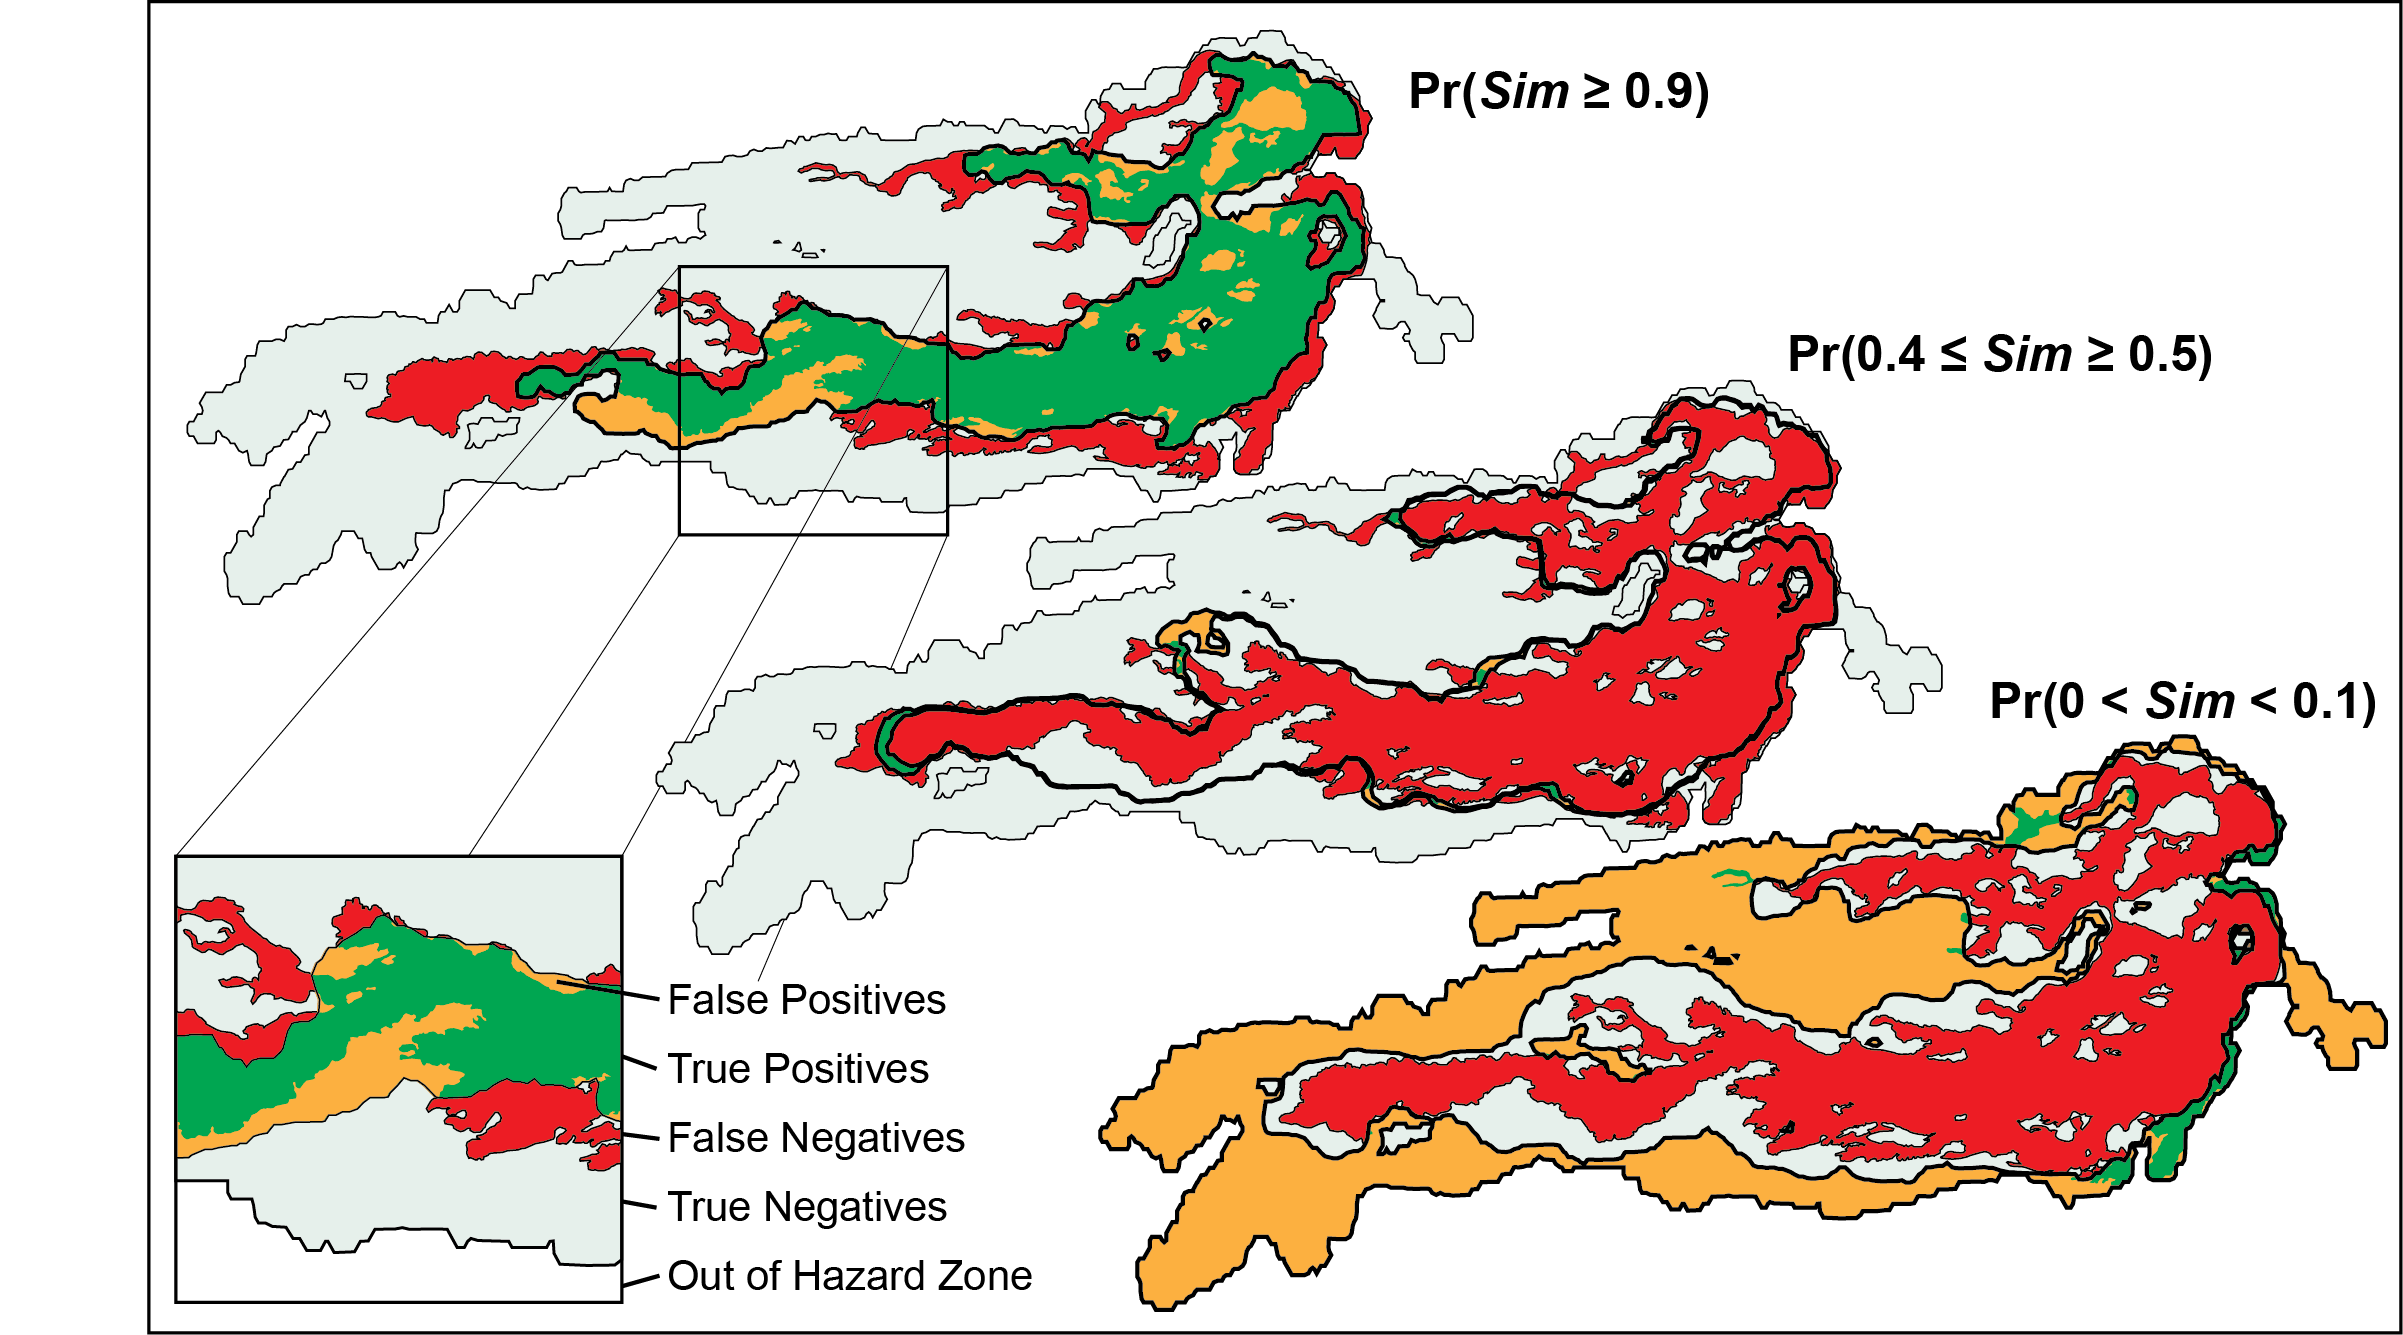
\includegraphics[width=0.7\linewidth]{\FigPath/PR_sim_examples_300dpi}
			\caption[Sub-regions within the Monte Carlo solution, defined by $\text{Pr}(Sim)$]{Sub-regions within the Monte Carlo solution, defined by $\text{Pr}(Sim)$. At the top, all areas inundated by $\ge$90\% of all simulations are shown in green (True Positives) and orange (False Positives). The remaining mapped lava flow (False Negatives) is red. The underlying region is the total Monte Carlo Hazard Area. At center, A thin band represents all areas inundated by 40-50\% of all Simulations. At bottom, a thick shell of areas rarely inundated by simulated lava is mostly orange, indicating rarely simulated flow areas are unlikely to have been inundated in real life.}
			\label{fig_MCsubregions}
		\end{figure}	
		
		It can be seen in Figure \ref{fig_MCsubregions} that most of the mapped flow is covered by the $\text{Pr}(Sim\ge90\%)$ sub-region, as the green true positive region is larger than the red false negative region. The sub-region defined as $\text{Pr}(0<Sim<10\%)$ does not spatially intersect with the mapped flow area as much as the $\text{Pr}(Sim\ge90\%)$ sub-region, and this can be seen in the lower right of Figure \ref{fig_MCsubregions} as the sub-region area is mostly orange false positives with small green true positive areas.
		
		The relative risk of inundation can be calculated for each subregion by comparing the probability of actual flow inundation $\text{Pr}(Lava)$ against the probability of not inundation $\text{Pr}(\neg Lava)$ using the Bayes Factor of Equation \ref{eq_BF}. Here ``Data'' is the probability of simulated inundation $\text{Pr}(Sim=\text{X})$, Model 1 is Real Flow Inundation and the opposing Model 2 is No Real Flow Inundation. For example, the relative probability of inundation for the sub-region defined by $\text{Pr}(40\le Sim<50\%)$ can be given as
		\begin{equation}
			\text{BF} = \frac{\text{Pr}(0.4\le Sim<0.5~|~\text{Inundation})}{\text{Pr}(0.4\le Sim<0.5~|~\text{Not~Inundation})}.
		\end{equation}
		The numerator $\text{Pr}(0.4\le Sim<0.5~|~\text{Inundation})$ is the probability of 40-50\% of simulations hitting a given location, given the location actually being hit by lava. Graphically, this is the percent of the true flow (red and green areas in the center example of Figure \ref{fig_MCsubregions}) that are within the simulated sub-region (green areas in the center example of Figure \ref{fig_MCsubregions}). The denominator $\text{Pr}(0.4\le Sim<0.5~|~\text{Not Inundation})$ is probability of 40-50\% of simulations hitting a location, given the location is not inundated in the real flow. This is the percent of the area not hit by the flow (light gray and orange areas in Figure \ref{fig_MCsubregions}) that is within the subregion (orange areas in Figure \ref{fig_MCsubregions}). 
		
		The probability that 40-50\% of simulations hit a location that is inundated is 2.7\%. The probability the 40-50\% of simulations hit a location that is not inundated by lava is 2.1\%. The Bayes Factor is then calculated to be 1.3, where the model of Inundation is 1.3 times more likely to describe this subregion than the model of Not Inundation. Referring to Table \ref{tab_BFinterps}, this result means that the preference for Inundation over Not Inundation is ``just worth a mention.'' Results for each 10\% wide sub-region are given in Table \ref{tab_BFresults} and are illustrated in Figure \ref{fig_bayesfactor}.
		

		\begin{table}
			\centering
			\caption{Relative likelihood of inundation given $\text{Pr}(Sim)$}
			\begin{tabular}{l c c c l}
				\toprule
				 & $\text{Pr}(Sim$=X$|$ & $\text{Pr}(Sim$=X$|$ & Bayes & \citet{jeffreys1998theory}\\
				X & $Lava)$ & $\neg Lava)$ & Factor & Interpretation \\
				\midrule
				$0<$X$<0.1$ & 0.06 & 0.67 & 0.09 & Strong evidence against inundation\\
				$0.1\le$X$<0.2$ & 0.02 & 0.08 & 0.23 & Substantial evidence against inund.\\
				$0.2\le$X$<0.3$ & 0.03 & 0.04 & 0.74 & No Inundation more likely\\
				$0.3\le$X$<0.4$ & 0.03 & 0.03 & 1.21 & Inundation more likely than not\\
				$0.4\le$X$<0.5$ & 0.03 & 0.02 & 1.29 & Inundation more likely than not\\
				$0.5\le$X$<0.6$ & 0.03 & 0.02 & 1.53 & Inundation more likely than not\\
				$0.6\le$X$<0.7$ & 0.04 & 0.01 & 2.63 & Inundation more likely than not\\
				$0.7\le$X$<0.8$ & 0.05 & 0.02 & 2.69 & Inundation more likely than not\\
				$0.8\le$X$<0.9$ & 0.06 & 0.02 & 2.84 & Inundation more likely than not\\
				$0.9\le$X$\le 1.0$ & 0.66 & 0.10 & 6.93 & Substantial evidence for inundation\\
				\bottomrule
			\end{tabular}
			\label{tab_BFresults}
		\end{table}
		
		\begin{figure}[!h]
			\centering
			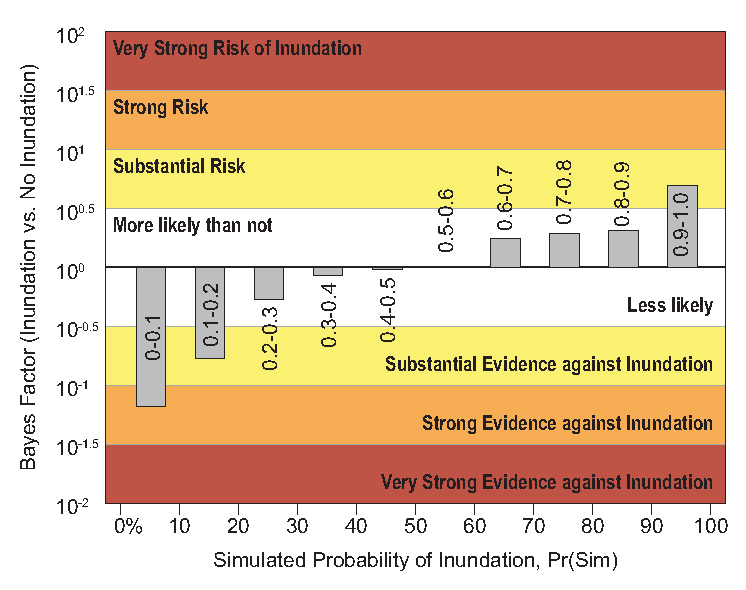
\includegraphics[width=0.7\linewidth]{\FigPath/LR_bayes}
			\caption[Relative likelihood of inundation given $\text{Pr}(Sim)$]{Relative likelihood of inundation given $\text{Pr}(Sim)$. Only locations inundated by $<10\%$ of Monte Carlo simulations show strong evidence against inundation in the actual 2012-3 Tolbachik lava flows.}
			\label{fig_bayesfactor}
		\end{figure}
		
		Only the sub-region least likely to be hit by simulations, where $\text{Pr}(Sim<10\%)$, has a Bayes Factor of $<10^{-1}$, which is interpreted as strong evidence against lava flow inundation. As the Bayes Factor can be treated as posterior odds for or against a model \citep{aspinall2003evidence}, a factor of $1/10$ indicates 10:1 odds against inundation. Sub-regions with factors greater than $1/10$, and are therefore more in support of flow inundation, have odds less than 10:1 against inundation. As 10:1 odds against inundation is the same as a probability of 9\% for inundation, all sub-regions besides the $\text{Pr}(Sim<10\%)$ sub-region have $\text{Pr}(Lava>9\%)$.
		


%%%%%%%%%%%%%%%%%%%%%%%%%%%%%%%%%%%%%%%%%%%%%%%%
%DISCUSSION
%%%%%%%%%%%%%%%%%%%%%%%%%%%%%%%%%%%%%%%%%%%%%%%%
%%%%%%%%%%%%%%%%%%%%%%%%%%%%%%%%%%%%%%%%%%%%%%%%
%%%%%%%%%%%%%%%%%%%%%%%%%%%%%%%%%%%%%%%%%%%%%%%%

\section{Discussion}\label{sec:discussion}
	\subsection{Benchmark Validation}
	Unique flow algorithms are validated by using common benchmarks that show whether these algorithms replicate expected lava flow morphologies under specific conditions. Different benchmark tests that are applicable to CA codes fall into three validation levels: 1) tests that show that simulations don't change when parameters remain meaningfully identical; 2) tests that show that simulations replicate experimental results or analytical expectations; and 3) tests that show that simulations replicate real world flow examples. A summary of the results of the eight algorithms against the example benchmarks are given below in Table \ref{tab_algorithmresults}.
		
	\begin{table}[h]
		\centering
		\caption{Transition Algorithm Results}
		\begin{tabular}{l | c | c | c c}
			\toprule
			Transition&\multicolumn{4}{c}{\textbf{Levels}}\\
			Function&1&2&\multicolumn{2}{c}{3}\\
			& DEM Rotation & Pancake & SRTM & TanDEM-X \\
			\midrule
			\textbf{4/P/S} & Pass & Fail & Pass & Pass\\
			\textbf{8/P/S} & Pass & Pass & Pass & Fail\\
			\textbf{4/N/S} & Fail & Fail & Pass & Fail\\
			\textbf{8/N/S} & Pass & Pass& Pass & Fail\\
			\textbf{4/P/E} & Fail & Ambiguous & Pass & Pass\\
			\textbf{8/P/E} & Fail & Ambiguous & Pass & Pass\\
			\textbf{4/N/E} & Fail & Pass & Pass & Pass\\
			\textbf{8/N/E} & Fail & Pass & Pass & Pass\\
			
			\bottomrule
		\end{tabular}
		\label{tab_algorithmresults}
	\end{table}
	
	Because these validation levels increase in complexity from Level 1 to Level 3, one possible strategy in validating different algorithms would be to only test algorithms at more complex benchmarks after they successfully pass less complex benchmarks. Valid models might then be determined by elimination. Only 3 of 8 tested algorithms pass the first ``rotating slope'' benchmark: 4/P/S, 8/P/S, and 8/N/S. Although more algorithms passed the second ``bingham flow on a flat surface'' benchmark, only 8/P/S and 8/N/S passed the previous benchmark and this one. Both of these flows then successfully replicated the Tolbachik lava flows over SRTM topography. Therefore the 8/P/S and 8/N/S algorithms hold up to three benchmark tests.
	
	Overall, in all tests 8-connected models outperform 4-connected models. While equal sharing algorithms outperform slope-proportional sharing on a flat slope, they fail on a rotating DEM and perform about the same on real topography. There does not seem to be an unambiguously better choice between using parent-child relationships or not. If future tests continue to show similar performance between models with and without parentage, other reasons can be used to choose a model, such as computer run-time. 
	
	The strength of the MOLASSES code is that new algorithms, such as those used in the SCIARA model \citep{crisci2004simulation}, can be implemented relatively quickly and run through the Benchmarking tests, which are written in Python. Combinations of implementation strategies can also be created on the fly by adjusting the makefile of the MOLASSES code instead of the code itself.

	\subsection{Bayesian applications for real lava flows}
		Validation of lava flow models is important as a method of increasing the value of models to forecast lava flow processes, thereby decreasing preventable loss. Flow models are generally improved by reducing false positives and false negatives while increasing the true positive area, which is the union of a flow simulation and real, mapped lava flows. Often, reducing one type of error comes at the cost of increasing another type. For example, by increasing the pulse volume parameter, false positives can be reduced while false negatives are increased (Figure \ref{fig:pulse_map}).
		
		A decision can be made as to whether false positives or false negatives are more important to reduce in calibrating a lava flow model. One possible decision would be to prefer the reduction of false negatives over the reduction of false positives, with the reason being that a forecast of inundation without eventual engulfment by lava (a false positive result) is bad, but an unexpected engulfment by lava (a false negative) would be worse.
		
		\subsubsection{Using Bayesian statistics to compare models}
		In Section \ref{sec_bayespulse}, an optimal pulse volume was defined as a volume that produced a simulated lava flow that had the highest posterior and negative posterior values. However, the pulse volume 14040 m$^3$ had the highest posterior value, while the pulse volume 4387 m$^3$ had the highest negative posterior value. The simple definition of ``optimal'' pulse volume does not seem to work.
		
		The best pulse volume might be decided based on a preference for reducing false negatives as discussed above. The posterior probability of inundation, $\text{Pr}(Lava|Sim)$ increases with increased true positives and decreases with increased false positives (Equation \ref{eq_simplepost}). It is essentially blind to false negatives. The negative posterior $\text{Pr}(\neg Lava|\neg Sim)$ probability is the opposite, increasing with increased true negative results, while decreasing with increased false negative results (Equation \ref{eq_simplenegpost}). 
		
		If false negatives are more important to reduce than false positives, more weight can be given to the negative posterior value of a simulation than the positive posterior value. In Figure \ref{fig_weightedposteriors}, the posterior and negative posterior values for each pulse volume (Figures \ref{fig_lavaGsim} and \ref{fig_neglavaGsim}) are used to produce weighted average scores of pulse volume. The extent to which false negative reduction might be preferred over false positive reduction is unknown, so four hypothetical weights are used. One of the weighted averages that is plotted assumes both posteriors are equally important in determining the best pulse volume parameter. The other three curves weight the negative posterior as being 2, 5, and 10 times as important as the positive posterior in scoring pulse volumes. Using these three weights, the highest scoring pulse volume is 4387 m$^3$ (Figure \ref{fig:pulse_map}b). If the two posteriors have equal importance, the highest scoring pulse volume is 14040 m$^3$ (Figure \ref{fig:pulse_map}c).
		
		\begin{figure}[h!]
			\centering
			\begin{gnuplot}[terminal=latex, terminaloptions=rotate]
				unset key
				set size 0.7,0.7
				set format xy "$%g$"
				set xlabel "Pulse Volume (m$^3$)" rotate by 90
				set ylabel "Model Score"
				set ytics 0.02
				set xtics 4000
				plot "results_bayes.dat" using 1:7 with points pt 1, "results_bayes.dat" using 1:5 with points pt 7, "results_bayes.dat" using 1:6 with points pt 3, "results_bayes.dat" using 1:4 with points pt 6
			\end{gnuplot}
			\caption[Weighted averages of $\text{Pr}(Lava|Sim)$ and $\text{Pr}(\neg Lava|\neg Sim)$ for different pulse volumes]{Weighted averages of $\text{Pr}(Lava|Sim)$ and $\text{Pr}(\neg Lava|\neg Sim)$ for different pulse volumes. Hollow circles, negative posterior ($\text{Pr}(Lava|Sim)$) is given 10$\times$ the weight of the posterior ($\text{Pr}(\neg Lava|\neg Sim)$); solid circles, 5$\times$ weight; asterisks, 2$\times$ weight; plusses, equal weight between posteriors. The highest scoring pulse volume is 4387 m$^3$ for all weight ratios except when both posterior values are weighted equally.}
			\label{fig_weightedposteriors}
		\end{figure}
		
	\subsubsection{Decision Making with the Bayes Factor}
	By dividing the Monte Carlo set of simulations of the Tolbachik lava flows into sub-regions based on $\text{Pr}(Sim)$, the relative likelihood of inundation was calculated (Figure \ref{fig_bayesfactor}). By using the Bayes Factor to compare likelihood of Indundation to Not Inundation, most sub-regions were not significantly better described by one model or the other. Only the sub-region of locations least likely to be hit by flow simulations had ``strong evidence'' against inundation, and only the sub-region of locations most likely to be hit by simulations had ``substantial risk'' of inundation. These results leave a large amount of ambiguity when making decisions to fortify or evacuate due to a lava flow.
	
	In discussing the decision making process for calling an evacuation due to an eruption at Mount Vesuvius, \citet{marzocchi2007probabilistic} provided a cost-loss model where two actions can be taken, protect and do not protect. Two costs are associated with these actions: $\mathcal{C}$ is the cost of protection and $\mathcal{L}$ is the cost of loss if the volcanic hazard occurs while a decision to not protect is made. If $\mathcal{L}$ is incurred, it is assumed to exceed cost $\mathcal{C}$, often because loss due to volcanic hazards includes the loss of life.
	
	\citet{marzocchi2007probabilistic} show that the minimum cost can be achieved if protection occurs when $p>\mathcal{C}/\mathcal{L}$ where $p$ is the probability of the hazard occuring. The ratio $\mathcal{C}/\mathcal{L}$ is hard to quantify because the socio-economic cost of lost lives or of lost trust in the government (in the case of false evacuations) is difficult to calculate, even though the physical cost of evacuation and the cost of infrastructure loss might be straight forward estimates. \citet{woo2008probabilistic} provided one estimate of $\mathcal{C}/\mathcal{L}=0.1$ at the very maximum if 10\% of people evacuated from an area would owe their lives to that evacuation. In this case, protection would be made when $p>0.1$.
	
	While lives are not commonly lost due to lava flows with the notable exceptions of Laki (A.D. 1783, Iceland) and Nyiragongo (A.D. 1977 and 2002, Democratic Republic of the Congo) \citep{peterson2000lava}, the ``protection threshold'' $p>0.1$ can still be used as an example. All Monte Carlo sub-regions have a probability of inundation ($\text{Pr}(Lava)$) greater than 0.1 except the sub-region $\text{Pr}(Sim<0.1)$ (Figure \ref{fig_bayesfactor}). If action to protect is made at $\text{Pr}(Lava>0.1)$, then evacuations or fortifications will be made for all locations inundated by $\ge$10\% of Monte Carlo simulations.
	
	Two Bayes-factor thresholds in Figure \ref{fig_bayesfactor} have odds against lava inundation at better than 10:1 (i.e. $\text{Pr}(Lava<0.1)$), ``strong evidence'' and ``very strong evidence'' against inundation. Given the hypothetical protection threshold of $p>0.1$, the decision to protect against a lava flow should be made for a location whenever the Bayes factor supporting inundation is $>10^-1$, or when there is less than ``strong evidence'' against inundation for that area. If the protection threshold is decided to be less than 0.1, then the evidence against inundation will have to be even stronger to support a decision to not protect an area. 
	
	It is unknown whether sub-regions defined as $\text{Pr}(Sim<0.1)$ should be expected to be relatively safe areas when using Monte Carlo results at future lava flow sites. To test the effectiveness of the MOLASSES algorithm used for the Tolbachik flows in other study areas, more example flows around the world will have to be tested.
		
		
\section{Conclusions}
	The MOLASSES framework used in this project provides a modular set of functions that can be interchanged to fundamentally alter the flow simulation algorithm. While only 8 different algorithms, which focused on simple variations in the transition function of Cellular Automata codes, were explored, different modules can feasibly be modified to change other flow characteristics (e.g. vent geometry, mass flux at source locations, temperature dependent flow).
	
	All CA and CA-like codes, including SCIARA \citep{crisci2004simulation}, MAGFLOW \citep{del2008simulations}, ELFM \citep{damiani2006lava}, LavaPL \citep{connor2012}, and MOLASSES share similarities. For instance, lava inundation is a binary condition for each location on a grid and source locations are set at defined grid cell coordinates. This enables a common set of benchmarks to be defined, which can be used to test the validity of all CA codes.
	
	Three validation levels have been identified and different benchmark tests have been given which apply to each level. After a code is successfully demonstrated to conserve mass, the first validation level ensures that the code does not change when parameters are changed in a meaningless way. The example benchmark is that simulated flows should not be slope-direction dependent. The second level compares simulations to analytical or experimental results. As lava flows on large scales are similar to Bingham fluids, a flow simulator should produce a circular pattern on a flat surface. The third and final level tests simulations against true lava flows. Here, the 2012-3 Tolbachik lava flow is used as an example, with flow parameters identified using TanDEM-X analysis \citep{kubanek2015lava}. It might only make sense to validate codes at higher validation levels once they have been sufficiently developed to be validated at lower levels.
	
	Two common fitness tests for lava flows are the Jaccard coefficient and model sensitivity. Model sensitivity gives the percentage of a mapped lava flow that a simulation successfully forecasts. A possible alternative to these tests is to use Bayesian posterior probabilities to evaluate the positive and negative predictive values of the simulation. These posteriors ($\text{Pr}(Lava|Sim)$ and $\text{Pr}(\neg Lava|\neg Sim)$ give the likelihood of flow inundation or not inundation given the simulation results.
	
	Once lava simulators have been successfully validated through benchmarking, these Bayesian statistics can be used to improve model input parameters and evaluate model uncertainty by incorporating uncertainty inherent in input parameters. It is also possible that the two posterior predictive values can be used to aid in decision making processes associated with active lava flow crises.
	
	
\section{Data Statement}
This code is available for free use on GitHub at the USFVolcanology page located at \url{https://github.com/USFvolcanology}, while the benchmarking codes can be found at \url{https://github.com/jarichardson/MOLASSES_benchmarking}. The MOLASSES code and the Benchmarking algorithms are kept in seperate self-contained repositories.

%\section{Acknowledgments}
%The development of this code was supported by SSI Grant

%%%%%%%%%%%%%%%%%%%%%
%References Section
\section{References}
\bibliography{molasses}
\bibliographystyle{apalike} 

%\begin{figure}
%\centering
%\includegraphics[width=\linewidth]{map_diff}
%\label{fig:map_diff}
%\end{figure}


\chapter[The Volcanic History of Syria Planum, Mars]{
The Volcanic History of Syria Planum, Mars \footnote{This chapter has been reprinted from the Journal of Volcanology and Geothermal Research with permission from Elsevier as: Richardson, J. A., Bleacher, J. E., Glaze, L. S., (2013), The Volcanic History of Syria Planum, Mars, Journal of Volcanology and Geothermal Research, 252, 1-13.}}\label{ch_syria}

\renewcommand*{\FigPath}{figures/chapter-syria_planum}

\section{Abstract}
A field of small (10s~km in diameter) volcanoes in the Syria Planum region of Mars is mapped to determine abundance, distribution, and alignments of vents.  These data are used to assess possible variations in eruption style across space and time. Each eruption site is assigned a point location. Nearest neighbor and two--point azimuth analyses are conducted to assess the spacing and orientations between vents across the study area. Two vent fields are identified as unique volcanic units along with the previously identified Syria Mons volcano.  Superposition relationships and crater counts indicate that these three volcanic episodes span $\sim$900 Ma, beginning in the early Hesperian and ending in the Early Amazonian. No clear hiatus in eruptive activity is identified between these events, although a progression from eruptions at Syria Mons, to regionally distributed eruptions that form the bulk of the Syria Planum plains, to a final migration of dispersed eruptions to Syria's northwest is identified. Nearest neighbor analyses suggest a non--random distribution among the entire population of Syria Planum, which is interpreted as resulting from the interaction of independent magma bodies ascending through the crust during different stress regimes throughout the region's eruptive history. Two--point azimuth results identify three orientations of enhanced alignments, which match well with radial extensions of three major tectonic centers to the south, east, and northwest of the study area. As such, Syria Planum volcanism evolved from a central vent volcano to dispersed shield field development over several hundred million years, during which the independent magma bodies related to each small volcano interacted to some extent with one or more of at least three buried tectonic patterns in the older crust.  These results show a strong relationship between independent mapping efforts of tectonic and volcanic features. Continued integration of volcano--tectonic mapping should provide direct constraints for future geodynamic models of magma production and thermal evolution of the Tharsis province.

\section{Introduction}
\label{sec-intro}

The Tharsis province is a volcanic rise extending over 4500 km across the western hemisphere of Mars, covering nearly a quarter of the planet's surface \citep{Hodges1994}. This region is suggested to display volcanic and tectonic activity into the late Amazonian \citep{Anderson2001,neukum2004recent} (Martian chronology is detailed briefly in Section \ref{sec:methodCrater}). The region is long recognized to include five major shield volcanoes, seven partly buried volcanoes, vast lava plains, and a wide range of smaller eruptive vents \citep{carr1977some,Greeley1981,MouginisMark1992,Hodges1994}. While twelve large named volcanoes are cataloged and their morphologies and morphometries described in detail \citep[and references therein]{Hodges1994,plescia2004morphometric}, small volcanic edifices (10s km in diameter) have received much less attention due to a lack of high resolution data with regional coverage prior to the Mars Global Surveyor (MGS) mission.

The acquisition of post--\textit{Viking} data enables for the first time detailed cataloging and morphologic descriptions of the wide range of small volcanic vents (hereafter referred to as small vents) in the Tharsis province \citep{baptista2008swarm,Baratoux2009,bleacher2007tharsis,bleacher2009spatial,Broz2012,Hauber2009,hauber2011very,Keszthelyi2008,Wilson2009}. This ability represents a critical step forward in the scientific understanding of Martian magma production and eruption. Because different types of volcanic features result from a combination of different eruptive conditions, magma and lava properties, and ambient variables \citep{greeley1977basaltic,WhitfordStark1982}, an understanding of the abundance and distribution of volcanic features serves as a fundamental framework that is needed to fully understand any volcanic system \citep{Head1981,Connor2000}.

Here we report on mapping and analyses of the vent fields within the Syria Planum region of Mars \citep{baptista2008swarm}. This is a portion of an ongoing investigation to catalog the location of small (10s km in diameter) vents across the Tharsis region.  Although each vent appears minor in areal coverage and volume compared to the larger Tharsis shield volcanoes, when considered together as vent fields comparable to the Snake River Plain in Idaho, USA \citep{greeley1977basaltic,Greeley1982}, they represent significant magma production events. In addition to the volume of lava visible on the surface, the entire crust of the Tharsis region appears to have been demagnetized \citep{Connerney2005,Lillis2006}. The passage of many small magma packages into and through the crust provides a plausible explanation for this demagnetization in areas that are hundreds of kilometers away from major shield volcanoes \citep{Lillis2009}.  Likewise, tectonic evidence has led to the suggestion that the Tharsis province has experienced multiple episodes of large mantle upwellings \citep{Plescia1982,mege1996plume,Anderson2001,Anderson2004,Wilson2002}, the centers of which are not necessarily spatially overlapping with major volcanoes.  \citet{Anderson2001,Anderson2004} refer to these events as magmatic-driven tectonic episodes, which is consistent with the identification of vent fields in the Tharsis plains.  As such, it is critical to assess the number, location, and duration of magma production events that contributed to the current morphology of the Tharsis region.

\subsection{Geologic Description}

Past mapping of Syria Planum has enabled the identification of several distinct units based on morphologic characteristics. \citet{baptista2008swarm} identified three distinct units in southwestern Syria: 1) a unit comprised of NW--trending graben, 2) lava flows associated with Syria Mons, and 3) a field of coalesced low shield volcanoes. The lava flows associated with Syria Mons are hundreds of kilometers in length and form kilometers--wide, finger--like sheets of lava throughout the unit. These flows embay the graben field, which is composed of narrow (100s of meters to kilometers) linear and curvilinear graben that are tens to hundreds of kilometers in length. The Syria Mons flows are crosscut by NE--SW trending graben, 10s of km in length. The coalesced shield field is composed of low shield volcanoes several kilometers in diameter that embay the Syria Mons lava flows. Both the field and the flows are crosscut with NW--SE trending graben (km in length). A newly identified geologic unit (Hnsf in Figure \ref{fig-geomap}) is located to the north of the \citet{baptista2008swarm} study area and is seen to embay the coalesced shield field to the south. It is characterized by lava flows tens to hundreds of kilometers in length emanating from a topographic ridge approximately 200km in length that trends NE--SW. The lava flows that form this unit are seen to fill preexisting graben that crosscut the southern coalesced shield field and embay vents from the southern shield field.

\begin{figure}
	\centering
	\includegraphics[width=0.8\linewidth]{\FigPath/fig1.eps}
	\caption[Geologic Map of Syria Planum]{Geologic Map of Syria Planum. The study area is shown inside the thick black line with a MOLA-derived hillshade basemap. The study area of \citet{baptista2008swarm} is shown as a rectangle in the south--central region of the study area. In the east a dotted line surrounds an area where no volcanic vents are found and is therefore not included in the study area (crater counting was not performed in this area). Volcanic vents are represented as a solid black point, likely volcanic vents as a white point outlined in black, and Syria Mons is represented as a star. Graben are shown as thin black lines. White lines separate geologic units. From north to south these units are: Hp, a unit on the margins of the plateau that features scattered individual vents; Hnsf, a northern shield field of coalesced volcanic vents; Hssf, a southern shield field of coalesced volcanic vents; Hsm, lava flows of Syria Mons; Hg, a graben-rich unit; Hlp, a unit of lava flows on the southeast margin of Syria Planum that hosts relatively few volcanic vents.}
	\label{fig-geomap}
\end{figure}

The mapping of \citet{baptista2008swarm} was limited by High Resolution Stereo Camera (HRSC) data availability to 100-105$^{\circ}$W, 13-23$^{\circ}$S within the Syria region. Despite this limitation, \citet{baptista2008swarm} demonstrated that analysis of high resolution image data with regional coverage showed new volcanic and tectonic complexities in this region that had previously been identified as a plains style volcanic province \citep{Sakimoto2003} similar to those described on the Earth \citep{Greeley1982}, and other Mars volcanic field studies \citep{bleacher2007tharsis,bleacher2009spatial,Hauber2009}. The addition of several tectonic episodes that temporally separate volcanic emplacement events leads to the hypothesis that Syria Planum is the surface product of multiple (opposed to one long--lived) magma production events. For clarity, we use the term ``magma production event'' to represent a broad magmatic upwelling that might feed multiple shallow, crustal magma bodies and small volcanic vents across a region like Syria. Such an event might be comparable to an event that feeds a major shield like Olympus Mons or each of the Tharsis Montes, and should be considered in models of the thermal and geologic evolution of Tharsis. Therefore, it is imperative to determine if a large field of vents like Syria represents one magma production event, or possibly multiple, temporally distinct events that are spatially overlapping on the surface of the planet.

In order to test this hypothesis we map volcanic vents in the full Syria Planum region at comparable resolutions to the study of \citet{baptista2008swarm}, which is only now possible due to the combined data acquisition of HRSC, Thermal Emission Imaging System (THEMIS), and Context Imager (CTX) images. Our objectives are to determine if multiple separable magma production events occurred in Syria and to assess whether these events can be clearly identified as unique events or the extension of a long--lived, continuous magma production event, either of which provide new insight into and modeling constraints for the thermal and tectonic evolution of the Tharsis province.

In this paper, new spatio--temporal boundaries of known volcanic units are presented and a new volcanic unit in the north of Syria is identified, separated from southern volcanism by a distinct flow margin. Each volcanic unit in Syria Planum is temporally constrained with superposition relationships and crater age--dating. Methods which are used to spatially describe small volcanic vents in Syria are then discussed, including nearest neighbor and 2--point azimuth statistical analyses. Finally, a revised volcano--tectonic history of Syria Planum is proposed, wherein we interpret that volcanism has likely migrated spatially throughout the evolution of Syria and wherein the style of volcanism has likely shifted from one central vent at Syria Mons to forming coalesced shield fields.

\section{Methods}

\subsection{Study Area}

The study area (Figure \ref{fig-geomap}), Syria Planum, is located on the southeastern margin of the Tharsis province between 8-23$^{\circ}$S and 110-93$^{\circ}$W. Syria Planum is bordered by Noctis Labyrinthus to the north, Claritas Fossae to the west and Solis Planum to the southeast. This area forms a regional plateau with a maximum elevation of 8000 m based on analysis of Mars Orbiter Laser Altimeter (MOLA) \citep{smith2003mars} gridded data. A total relief of 4000 m exists between this point and the southeastern portion of the study area. The study area is roughly 1000 by 900 km in size as defined by \citet{Scott1986}, with an abundance of volcanic vents focused in an area roughly 700 by 600 km in size \citep{Richardson2010,Richardson2012}. In order to characterize the volcanic evolution of Syria all identifiable volcanic vents in the study area are mapped and morphologic units are identified as temporally separable by crater counting. Nearest neighbor and 2--point azimuth statistical analyses are applied to the vent location data to provide additional constraints on the evolution of the volcanic region. A 512 pixels--per--degree (ppd) THEMIS infrared (IR) day--time mosaic \citep{Christensen2004} and the 128 ppd MOLA gridded dataset \citep{smith2003mars} are used as base maps. Relevant CTX \citep{malin2007context} and THEMIS visible (VIS) \citep{Christensen2004} images are co-registered to this base map for the identification of volcanic vents.

\subsection{Catalog of Volcanic Vents}

Volcanic vents are spatially cataloged as single points in a Cartesian grid, referencing their plan view position with respect to the THEMIS IR day--time mosaic and the gridded MOLA dataset base maps. Each datum is assumed to closely represent the four--dimensional (space and time) pathway along which magma ascended through the crust to erupt at the surface and produce an identifiable vent structure \citep{Bishop2007}. Volcanic vents are here defined as positive topographic landforms, tens to hundreds of meters in height, with flows or flow--like textures radiating from the apex and/or depressions at the topographic summit. Many positive topographic landforms lack clear flow features or a preserved depression at the apex, but are otherwise morphologically similar to cataloged vents. These landforms, which are tens to hundreds of meters in height, are also cataloged as likely volcanic vents (an example with contours is shown in Figure \ref{fig-geomap}). It is assumed that many volcanic vents that formed within the volcanic field on Syria Planum have since been buried by continued volcanism. This mapping project does not consider these buried vents, nor does this study provide any assumptions about stalled magma bodies for which ascension pathways were established but did not lead to surface eruptions (in other words, the intrusion to extrusion ratio of the region as was estimated in southern Tharsis by \citet{Lillis2009}). Instead, vents that are currently identifiable on the surface are assumed to represent the last stage of eruptive activity in the region and are used to provide new insight into the magmatic and volcanic history of Syria and the Tharsis province.

A variety of volcanic vent morphologies are present on Tharsis and have recently been characterized using post--\textit{Viking} era image data \citep{bleacher2007tharsis,bleacher2009spatial,Broz2012,Keszthelyi2008,baptista2008swarm,Hauber2009,Wilson2009,Baratoux2009}. Different methods are implemented for different vent morphologies to realistically assign a representative two--dimensional point to this four--dimensional process. For volcanic vents with depressions at the summit from which lava has visibly erupted (based on interpretation of radiating textures or buildup of spatter or cinder rims (examples in Figure \ref{fig-geomap})) a data point is digitally created  at the center of the depression using ArcGIS 9.3. For volcanic vents with linear depressions along a topographic high, the data point is created at the midpoint of a line with endpoints at the extents of the depression. In cases where the depression extends beyond the apparent eruptive activity (in other words, an extended dry fracture associated with the eruptive segment of the fissure as discussed by \citet{greeley1977basaltic} in volcanic fields) the data point is assigned at the middle point of a line connecting the ends of the eruptive segment. For likely volcanic features, which do not display summit depressions, data points were assigned at the topographic summit of the feature or at the origin of radiating flow textures where possible.

Cataloging the location of volcanic vents within Syria also enables the identification of distinct large scale flow features and units based on different morphological and superposition characteristics.  Consistent superposition relationships among vent groups within Syria are identified. Using the map of vent locations (Figure \ref{fig-geomap}) and superposition relationships for Syria Planum, several techniques are applied to further characterize the region's eruptive history. Based on the identification of unique vent groups, crater counts (described in Section \ref{sec:methodCrater}) are conducted to test whether quantifiable hiatuses occurred between the formation of different volcanic and tectonic events. Nearest neighbor analysis (described in Section \ref{sec:methodNN}) is applied to the complete Syria vent catalog and to subgroups of vents within the study area based on morphological mapping units. Nearest neighbor analysis is applied to assess the spatial distribution among vents. This has been shown as a method of characterizing a group of data points as being composed of one or a combination of populations \citep{Bishop2007, Baloga2007}. A two--point azimuth technique (described in Section \ref{sec:methodAzimuth}) is implemented to identify potential lineaments between volcanic vents that might correlate to underlying structures \citep{Lutz1986,Wadge1988,Wadge1989,connor1990cinder,lutz1995improved,bleacher2009spatial} in an attempt to better understand the ascent of magma beneath Syria. The combination of such spatial and alignment analyses has been used to characterize volcanic fields on the Earth \citep{Lutz1986,lutz1995improved,Cebria2011,Roberts2011} and Mars \citep{bleacher2009spatial}.

\subsection{Crater Counting}
\label{sec:methodCrater}

Using the 512ppd THEMIS infrared daytime mosaic, craters larger than 0.5~km in diameter are cataloged in accordance with identified vent groups and morphologic units. For each morphologic unit, a crater retention age is fitted to a cumulative crater size--frequency distribution following the method described in \citet{hartmann2005martian} and using the freely available software Craterstats2 \citep{Michael2010}. The size--frequency distribution is fit to a production function from \citet{Ivanov2001} and an absolute age is calculated using the chronology model from \citet{Hartmann2001}.

Given the relatively large surface area of each morphologic unit (e.g. one unit is composed of $>$100 volcanic shields) and the relatively low spatial resolution of the THEMIS mosaic (100~m), isochrons for this study are fit using craters of diameter $\ge$1~km. Craters of diameter $<$1~km are not used for determining ages due to the tendency for the number of smaller craters to artificially diminish as their diameter approaches the resolution of the base map.s Crater retention rates are reported with errors following the equation
\begin{equation}
N(1) = \frac{n_{1km}}{A} \pm \frac{\sqrt{n_{1km}}}{A} \label{eq1}
\end{equation} 
where $n_{1km}$ is the observed number of craters with diameters greater than 1 km and $A$ is the surface area in km$^2$.

Ages determined by crater age--dating are assigned an epoch range based on the Martian chronostratigraphic system as recently outlined by \citet{Werner2011}. Generally, the three periods of the Martian system are the Noachian, Hesperian, and Amazonian, ranging from $>$3.96-3.57~Ga, 3.57-3.00~Ga, and 3.00~Ga-present, based on the chronology model of \citet{hartmann2005martian}, respectively. These periods are further separated into epochs as follows: Middle Noachian, 3.96-3.85~Ga; Late Noachian, 3.85-3.57~Ga; Early Hesperian, 3.57-3.40~Ga; Late Hesperian, 3.40-3.00~Ga; Early Amazonian, 3.00-0.88~Ga; Middle Amazonian, 0.88-0.24~Ga; Late Amazonian, 0.24~Ga to present.

\subsection{Nearest Neighbor Analysis}
\label{sec:methodNN}

The distances from each volcanic vent to its nearest neighboring vent in a volcanic field can be used to characterize the spatial distribution of the volcanic vents within a field. It has been hypothesized that the vents of a terrestrial volcanic vent field (i.e. field volcanism) will conform to a random spatial distribution \citep{Lutz1986,lutz1995improved}. This is to say that each vent is located in the study area independently of the location of any other vent, that each vent has the same probability of occurrence at any location in the study area, and that any subarea of the study area is equally likely to contain any vent as any other identically sized study area \citep{Clark1954}.

Based on the Poisson spatial distribution, \citet{Clark1954} defined two statistics with which to analyze nearest neighbor (NN) distances for a spatial distribution of points. First, the test statistic, $c$, is given by the equation 
\begin{equation}
c= \frac{\bar{r}_a -\bar{r}_e}{\sigma_e},  \label{eq3}
\end{equation}
where $\bar{r}_a$ is the mean observed NN distance, $\bar{r}_e$ is the expected mean NN distance for a Poisson spatial distribution, and $\sigma_e$ is the expected standard deviation of NN distances. Expected values of $c$ were simulated by \citet{Baloga2007} to remove bias based on sample size. If the observed $c$ statistic departs from the expected $c$ by more than $2\sigma$ for the appropriate sample size, spatial randomness may be rejected.

Second, the ratio between the observed mean NN distance, $\bar{r}_a$, and the expected mean NN distance, $\bar{r}_e$, given by equation \ref{eq4}, also tests the fit of Poisson randomness.
\begin{equation}
R = \frac{\bar{r}_a}{\bar{r}_e} \label{eq4}
\end{equation}
If a vent field is spatially random in a Poisson sense, the $R$-index will approach 1. Values of $R~>$~1 suggest that the points approach maximal packing, while values of $R~<$~1 suggest that points are more clustered than expected for a Poisson spatial distribution. Similar to the test statistic $c$, the calculated $R$--index may be compared to an expected $R~\pm~2\sigma$ to test for the fit of Poisson randomness to describe the distribution of points.

\citet{Baloga2007} also developed a test using the skewness and kurtosis of the NN distribution to further constrain the applicability of the Poisson distribution to a spatial sample. Using 1000 simulated Poisson point sets of the same sample size, it was observed that skewness and kurtosis are strongly correlated and focus around an elliptical centroid.  If the skewness and kurtosis values for a given point set plot sufficiently far away from the centroid of simulated Poisson values, randomness in the Poisson sense may again be rejected.

Nearest neighbor analysis described above can be used to quantitatively compare the spatial distribution of volcanic vents with the null hypothesis, H$_o$, of spatial randomness in a Poisson sense. We hypothesize that if the vents are spatially random in the Poisson sense, then the vents have formed independently of each other as part of one larger magma production event (e. g. their respective magma ascension pathway through the crust was not influenced by the location of any other vent thereby causing a random spacing of eruption points). If a Poisson distribution is rejected and the $R$--index statistic shows evidence for clustering, we interpret the result as evidence that multiple temporally distinct magma production events have occurred beneath Syria Planum that are spatially overlapping, thereby resulting in two or more random but mixed statistical populations \citep{Lutz1986,lutz1995improved}.

To perform nearest neighbor analysis, Geological Image Analysis Software (GIAS), version 1.12, was used \citep{Beggan2010,Hamilton2010,Hamilton2011}.

\subsection{Two--point azimuthal analysis}
\label{sec:methodAzimuth}

Two--point azimuth techniques have been used to observe and describe lineaments between volcanic vents for decades \citep{Lutz1986,Wadge1988,Wadge1989,connor1990cinder,lutz1995improved,bleacher2009spatial,Cebria2011,Roberts2011}. Azimuth techniques determine the directions from each point to every other point. Lineaments between vents are identified by looking at anomalously high numbers of azimuths in any given direction and comparing that with other linear features, such as faults and graben, observed in the area or in adjacent, older terrains for which their traces might have been buried by the emplacement of the volcanic field or other geologic processes.

\citet{Cebria2011} postulated that lineaments between two vents are more likely if those vents are relatively close to each other. They therefore suggested that two point azimuth techniques should use a \textit{minimum significant distance}, a distance where the azimuths of closer inter--vent relationships best characterize lineaments of the given field. Inter--vent relationships farther than this minimum significant distance are not as likely to be related by the same underlying geological structures. Adding to the benefit of using only inter--vent relationships smaller than this distance is that anomalously far inter--vent relationships will likely display bias in the direction of the vent field's major axis. If the vent distribution for example, resembles a narrow ellipse due to topographic focusing, the longer inter--vent relationships will necessarily point in the direction of the long axis of the ellipse even if regional tectonic patterns are perpendicular.

For this study, the minimum significant distance used is defined by \citet{Cebria2011}
\begin{equation}
d \le (\mu_v - 1\sigma_v) / 3 \label{eq5}
\end{equation}
where $\mu_v$ is the mean inter--vent distance and $\sigma_v$ is the standard deviation of inter--vent distances. Using the set of inter--vent relationships shorter than this distance, relationships are grouped by direction into nine bins of a rose diagram. We hypothesize that bins containing an anomalous amount (count~$\ge~\bar{x}_n~+~\sigma_n$) of inter--vent relationships are evidence of lineaments between vents. These orientations are compared with regional tectonic trends as possible influences of magma ascension \citep{bleacher2009spatial,Cebria2011}.

\section{Results}

\subsection{Mapping}

In the study area 263 vents are identified, with 206 cataloged as volcanic vents and 57 cataloged as likely volcanic vents. There is no specific area where likely volcanic vents (as opposed to volcanic vents) are concentrated, though the highest abundance of likely volcanic vents are in northern Syria Planum. Because of the likely volcanic vents' regional distribution and topographic similarity to landforms cataloged as volcanic vents, we have included likely volcanic vents in the statistical analysis of all volcanic vents on Syria Planum. Here after both categories of vents are treated as one catalog, which includes 263 features.

The 263 identifiable vents within Syria Planum are distributed among five of six identified map units on Syria, which are delineated based on observed superposition relationships. Cataloged volcanic vents, geologic units, and graben are plotted in Figure \ref{fig-geomap}. A graben--rich unit previously described by \citet{baptista2008swarm} and \citet{Tanaka1988}, Hg, is located in the southwest of the study area and is seen to be embayed by the lavas of the Syria Mons unit, Hsm. Lavas associated with Syria Mons cover much of the study area and extend at least several hundreds of kilometers from Syria Mons' main vent towards the southeast. The Syria Mons summit is the only vent cataloged in this unit. The boundaries of the Syria Mons unit are defined to the west and south by the margins of distinct, overlying lava flows. To the east, the Syria Mons unit is embayed by low shields that coalesce into a volcanic vent field, Hssf. Syria Mons and thirty volcanoes that make up this coalesced vent field unit were extensively mapped by \citet{baptista2008swarm}. The majority of vents cataloged in Syria Planum, 192, are cataloged in this vent field. Low shields that coalesce to form this unit have slopes 1-2.5$^{\circ}$ and diameters between 10 and 35 kilometers. Eight vents are identified in this unit that have slopes up to 6$^{\circ}$ and diameters of 2-10~km. The low shields of this unit extend into the southeast where they flow over a unit of large scale lava flows, Hlp, that extend from a center within Syria Planum, which is unrecognized at this time. In this southeastern unit, 6 vents are cataloged.

To the north of the coalesced unit are distinct flow margins. The lava that created these flow margins embay low shields associated with the coalesced unit and fill graben that have cross--cut the coalesced unit. The source of the embaying lava flows to the north is a unit comprised of 22 vents that form a second coalesced volcanic vent field. To distinguish between these two coalesced volcanic units, the field to the south, Hssf, is labeled as the ``southern shield field'' and the field to the north, Hnsf as the ``northern shield field.'' The northwestern boundary of the northern shield field is determined by the extent of visible lava flows, which extend to the north and south of the vents as far as 200~km. The northwest region of the study area is identified as one unit, Hp, beyond the lava flows of Syria Mons and the northern shield field. The northwestern unit contains 42 vents, which do not coalesce together to make one distinct field. The relative superposition of this unit to the Syria Mons lava flows and the northern shield field are not clearly defined.

\begin{table}
\centering
\caption{Summary of Vent Counts in Defined Units}
\label{tab-ventct}
\begin{tabular}{l c c c}
\toprule
& Volcanic Vents & Likely Volcanic Vents & Total Vents  \\
\midrule
Northern Shield Field, \textit{Hnsf}$^*$ & 13 & 9 & 22 \\
Southern Shield Field, \textit{Hssf}$^*$ & 159 & 33 & 192 \\
Syria Mons Unit, \textit{Hsm} & 1 & 0 & 1 \\
Northwest Syria Planum, \textit{Hp} & 28 & 14 & 42 \\
Southeast Syria Planum, \textit{Hlp} & 4 & 2 & 6 \\
\midrule
Totals & 205 & 58 & 263 \\
\bottomrule
\multicolumn{4}{p{0.95\linewidth}}{$^*$Nearest neighbor analysis is performed on the vent populations of the northern and southern shield fields and the combination of these fields.}
\end{tabular}
\end{table}


The vents of the two coalesced shield fields are identified as subgroups within the catalog of Syria Planum vents and are used for statistical analysis in this study. The locations of volcanic vents cataloged in the study area are summarized in Table \ref{tab-ventct}. Because the flow fronts farthest from, but still associated with, the northern shield field are buried by successive flow fronts closer to the observed vents of the shield field, their temporal connection to the observed vents is not confirmable. For this reason, geologically lower flow fronts which are embayed by flows and are not able to be connected to northern shield field vents are described as intermediate flows in age--dating exercises discussed in Section \ref{sec:resultsAgeDating}.

\subsection{Age--Dating}
\label{sec:resultsAgeDating}

\begin{table}
\centering
\caption{Crater Retention Rates and Ages for Selected Units}
\label{tab-crater}
\begin{tabular}{l c c l}
	\toprule
  & 10$^{-3}$~N(1) & Age, & Epoch$^*$\\
  & craters~km$^{-2}$ & Ga &\\
  \midrule
  Northern Shield Field, \textit{Hnsf} & 1.4$\pm$0.2 & 2.56-3.23 & Late Hesp. to Early Amaz. \\
  Northwest Syria Planum, \textit{Hp} & 1.5$\pm$0.1 & 3.17-3.29 & Late Hesp. \\
  Intermediate Flows, \textit{Hnsf?} & 1.7$\pm$0.4 & 3.28-3.52 & Early to Late Hesp. \\
  Southern Shield Field, \textit{Hssf} & 1.7$\pm$0.1 & 3.23-3.35 & Late Hesp. \\
  Southeast Syria Planum, \textit{Hlp} & 1.8$\pm$0.1 & 3.33-3.40 & Late Hesp. \\
  Syria Mons Unit, \textit{Hsm} & 2.0$\pm$0.1 & 3.41-3.47 & Early Hesp. \\
  Graben Basement, \textit{Hg} & 2.2$\pm$0.2 & 3.37-3.46 & Early to Late Hesp.\\
	\bottomrule
	\multicolumn{4}{p{0.95\linewidth}}{$^*$Hesp.: Hesperian; Amaz.: Amazonian.}
\end{tabular}
\end{table}

In Table \ref{tab-crater} and illustrated graphically in Figure \ref{fig-unitages}, crater counts and their corresponding age-dates are presented. According to these counts, the last lava flowed over the surface of Syria Planum as recent as the early Amazonian. Crater dating also shows that the lavas from Syria Mons and the graben--rich basement that they embay, which are the lowest observed geologic units, were last significantly resurfaced during the early Hesperian epoch.

\begin{figure}
\centering
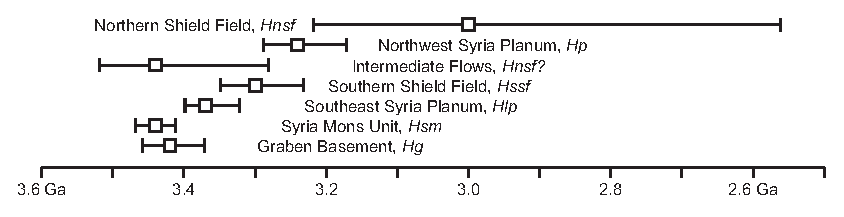
\includegraphics[width=0.7\linewidth]{\FigPath/fig2.eps}
\caption{Graphical summary of age--dating results by unit.}
\label{fig-unitages}
\end{figure}

Using superposition, volcanic units are relatively dated with Syria Mons erupting first, low shields of the southern shield field embaying its flows, and lavas of the northern shield field embaying the southern shield field. As shown in Figure \ref{fig-unitages}, error bars between ages of flows associated with Syria Mons, the southern shield field, and the northern shield field do not overlap and are in agreement with superposition observations. However, no significant haitus exists between the development of each unit. While some units seem ambiguously dated with respect to superposition (e.g. the graben--rich basement unit upon which are flows from Syria Mons is dated to be younger than the Syria Mons flows), no unit is in direct disagreement with relative dating observations, within error.

\subsection{Nearest Neighbor Analysis}

\begin{figure}
\centering
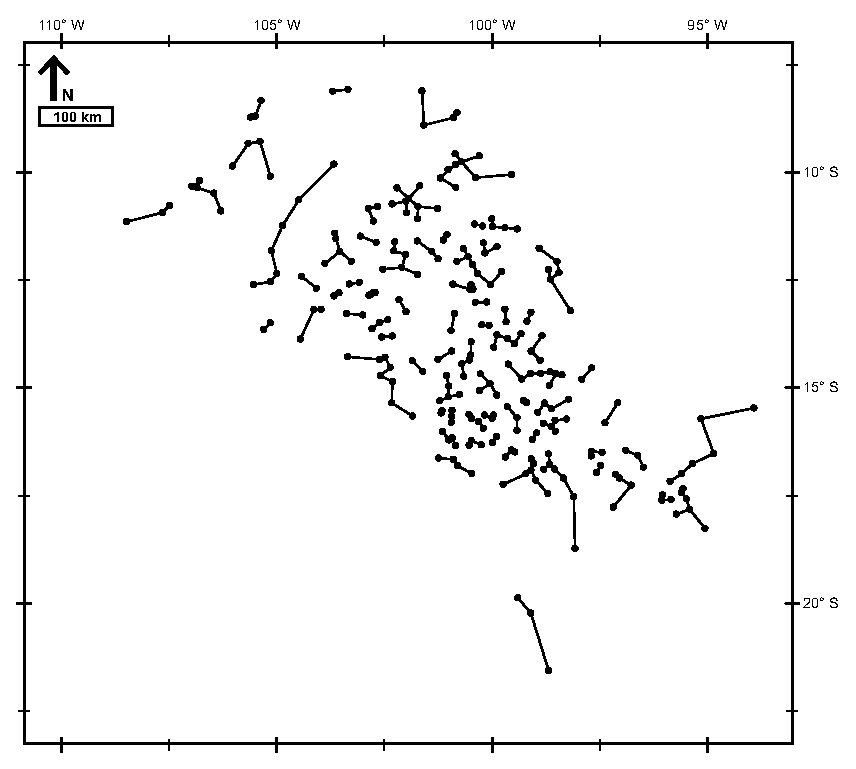
\includegraphics[width=0.5\linewidth]{\FigPath/fig3.eps}
\caption{Plot of vents with lines drawn to their nearest neighbors.}
\label{fig-nnmap}
\end{figure}

Figure \ref{fig-nnmap} is a map of all vents cataloged in Syria Planum with lines drawn to represent the connections from each vent to their nearest neighbor. Nearest neighbor analysis is conducted using these distances. Table \ref{tab-nn} presents results of the nearest neighbor analyses. The first two columns of Table \ref{tab-nn} give the expected and observed nearest neighbor distances for each area examined. The columns for $R_e$ and $c_e$ give the acceptance ranges for values of $R$ (defined in Equation \ref{eq4}) and $c$ (defined in Equation \ref{eq3}), respectively, based on sample size. The results of the skewness/kurtosis test are plotted in Figure \ref{fig-skgraphs}. Each plot shows simulated values of skewness and kurtosis for 1000 random Poisson spatial distributions (in gray). When the black diamond (indicating observed skewness and kurtosis values) falls within the gray area, this indicates consistency with Poison randomness. Inferences based on the skewness/kurtosis values shown in Figure \ref{fig-skgraphs} are summarized in the last column of Table \ref{tab-nn}.

\begin{table}
\centering
\caption{Summary of Nearest Neighbor Analysis on Cataloged Vents and two Subgroups of Vents}
\label{tab-nn}
\begin{tabular}{p{3cm} c c c c c c c}
	\toprule
  & $\bar{r}_e$ & $\bar{r}_a$ & $R_e$ & $R$ & $c_e$ & $c$ & S/K Plot \\
  \midrule
  All Syria Planum      & 18.7 km & 16.5 km & 1.03$\pm$0.07 & 0.88 & 0.80$\pm$2.14 & -3.57 & rejected \\
  N\&S Shield Fields    & 13.6 km & 14.7 km & 1.03$\pm$0.08 & 1.11 & 0.82$\pm$2.14 & 2.20 & rejected \\
  Southern Shield Field & 13.6 km & 15.4 km & 1.03$\pm$0.09 & 1.09 & 0.83$\pm$2.15 & 2.29 & accepted \\
  Northern Shield Field & 14.9 km & 12.3 km & 1.15$\pm$0.39 & 1.25 & 0.97$\pm$2.57 & 1.82 & accepted \\
	\bottomrule
	\multicolumn{8}{p{0.95\linewidth}}{$\bar{r}_e$, the expected mean NN distance; $\bar{r}_a$, the observed mean NN distance; $R_e$, the expected $R$-index and acceptance range; $R$, the observed $R$-index value (from Equation \ref{eq4}); $c_e$, the expected $c$ statistic and acceptance range; $c$, the observed $c$ statistic (from Equation \ref{eq3}). The final column lists the results of the skewness/kurtosis plot tests, testing the null hypothesis of Poisson spacing at the 0.05 significance level.}
\end{tabular}
\end{table}

\begin{figure}
\centering
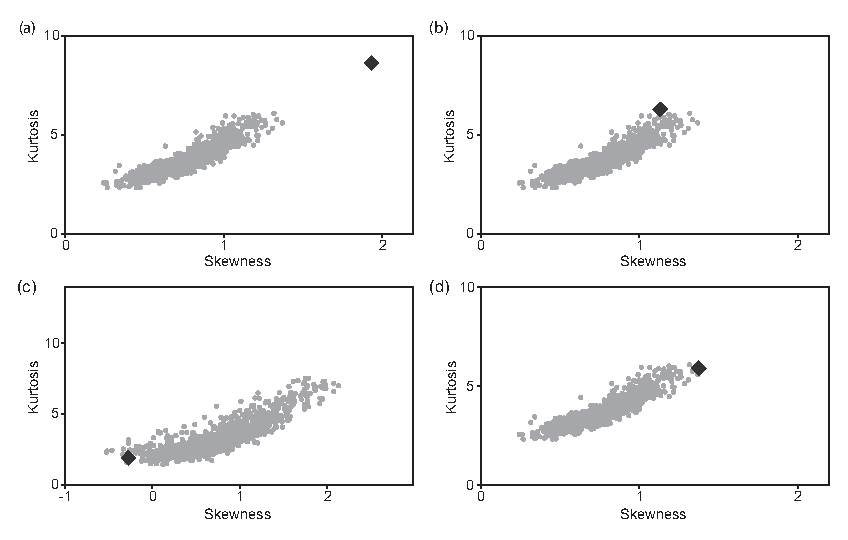
\includegraphics[width=0.5\linewidth]{\FigPath/fig4.eps}
\caption[Plots of skewness vs. kurtosis values for 95\% of 1000 simulated Poisson spatial distributions]{Plots of skewness vs. kurtosis values for 95\% of 1000 simulated Poisson spatial distributions. Diamonds represent the corresponding experimental values for a) all cataloged vents on Syria Planum, b) vents in both shield fields, c) vents in the northern shield field, and d) vents in the southern shield field. Randomness is rejected for all vents and for the combined shield fields (a, b respectively) at the 0.05 significance interval and accepted for both shield fields (c,d) individually. Simulated Poisson spatial distributions for a, b, and d use 300 data points; for c, 30 data points.}
\label{fig-skgraphs}
\end{figure}

All cataloged vents in the study area are first analyzed as a single group to test the null hypothesis, $H_o$, that the vents are spatially random in a Poisson sense. Spatial randomness of the entire study area could be evidence that a single magma production event may explain all volcanism in Syria Planum. However, due to the low $R$--index, the low $c$ statistic, and the result of the skewness/kurtosis test where the field plotted outside the range of Poisson randomness at the 99\% confidence interval, we reject the null hypothesis that the vents on Syria Planum are consistent with a Poisson spatial distribution when the entire study area is considered. Moreover, the observed $R$--index indicates that for all of Syria Planum the vents have a tendency to cluster, which is evidence that multiple subgroups might be identified as independent magma production events.

A subgroup that includes vents in both the northern and southern shield fields is also examined. Nearest neighbor results of this subgroup (N \& S row in Table \ref{tab-nn}) inconclusively characterize the randomness of the combined field. The observed $c$ statistic is within the predicted range, the $R$--index is calculated to be at the limit (\textit{R} = 1.11) of the expected $R \pm 2\sigma$, and the skewness and kurtosis values deviate from the elliptical centroid enough to reject randomness at the 0.05 significance level.

The vents within the northern shield field and the southern shield field are also analyzed individually to test their spatial randomness (Table \ref{tab-nn}). According to all three tests (the $R$--index, the $c$ statistic, and the skewness/kurtosis test) both the northern shield field and the southern shield field are found to exhibit Poisson spatial randomness individually. Therefore the null hypothesis of spatial randomness cannot be precluded for these shield fields. It is important to note that the northern shield field includes only 22 vents, increasing uncertainty in this conclusion. However, as the  southern shield field (n = 192) clearly exhibits spatial randomness and the combination of the two shield fields produces an ambiguous spatial distribution, there is evidence to suggest that the two shield fields are statistically distinct.

\subsection{Two--point azimuthal analysis}


\begin{figure}
\centering
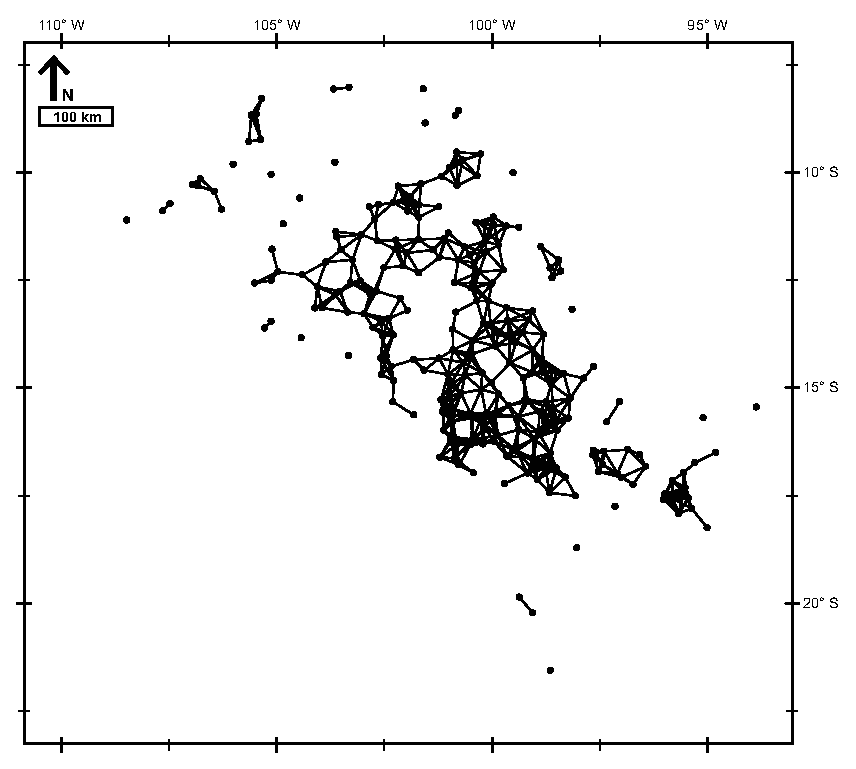
\includegraphics[width=0.5\linewidth]{\FigPath/fig5.eps}
\caption{Plot of vents and all inter--vent relationships less than the minimum significant distance.}
\label{fig-azmap}
\end{figure}

Figure \ref{fig-azgraphs}a displays a histogram of the lengths of all 34,453 inter--vent relationships. The skewness of this set of distances is 0.79. The mean distance, $\mu$, is 267~km and the standard deviation, $\sigma$, is calculated to be 157~km. The relationships used to investigate lineaments are below the minimum significant distance of $\le$~36.9~km as defined in Equation \ref{eq5} \citep{Cebria2011}. The number of inter--vent relationships, n, below the minimum significant distance, is 745. Figure \ref{fig-azmap} is a diagram of the vents represented as points in two-dimensional Cartesian space, using their locations in meters, and relationships between vents that are below the minimum significant distance.


\begin{figure}
\centering
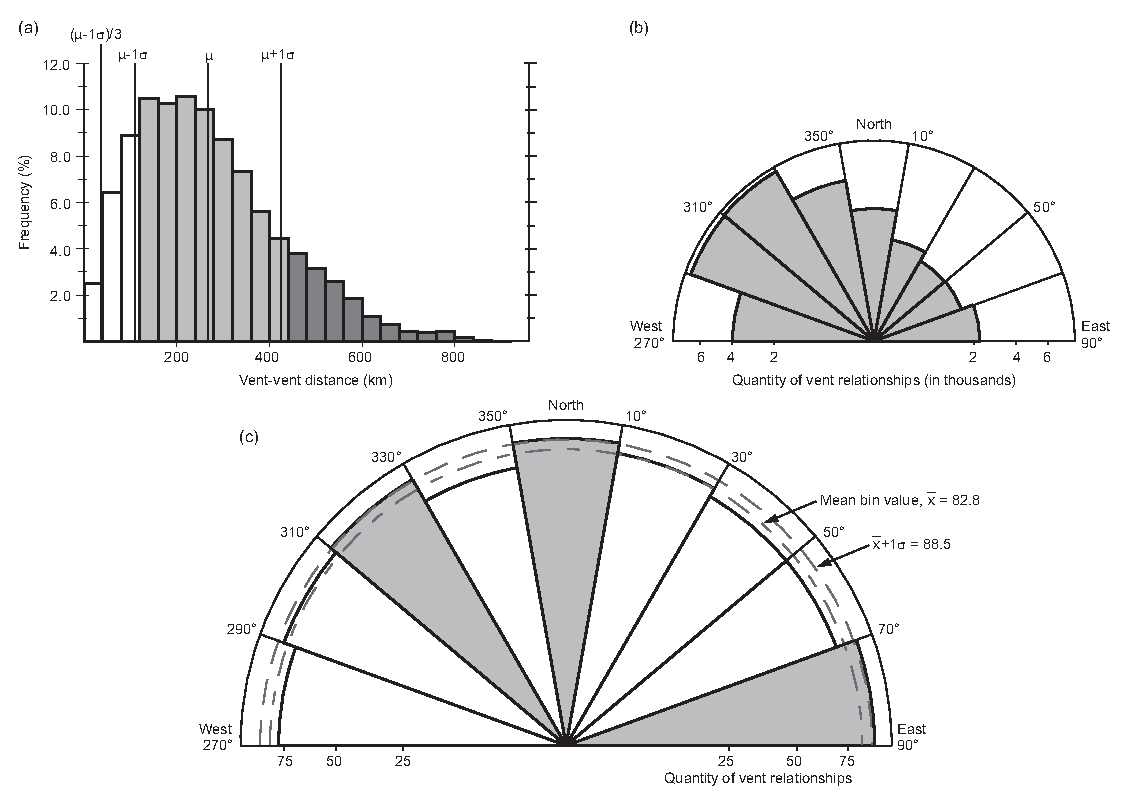
\includegraphics[width=0.7\linewidth]{\FigPath/fig6.eps}
\caption[Distribution of inter--vent distances and inter--vent alignments]{a) Distribution of inter--vent distances. Azimuths of inter--vent relationships are used if the inter--vent distance is less than 39.6 km, the defined minimum significant distance. Distances shaded dark gray are anomalously long and might trend in the overall vent field. Distances shaded light gray are of moderate length and are considered to be background noise. b) Directional distribution considering all inter--vent relationships. The plotted northwest mode is a result of including long distance inter--vent relationships. c) Direction distribution of inter--vent alignments below the minimum significant distance. The inner dotted line represents the mean quantity of inter--vent relationships. The outer dotted line represents the quantity of relationships one standard deviation above the mean. Directional wedges shaded gray (70-90$^{\circ}$, 310-330$^{\circ}$, 350-10$^{\circ}$) have anomalously high quantities of inter--vent relationships.}
\label{fig-azgraphs}
\end{figure}

The rose diagram in Figure \ref{fig-azgraphs}c illustrates the results of categorizing relationships based on the direction. The mean quantity of relationships in each direction bin, $\bar{x}_n$, is 82.8 and the standard deviation, $\sigma_n$, is 5.74. Three bins are identified as containing heightened amounts (count $\ge \bar{x}_n + \sigma_n$) of inter--vent relationships: 70-90$^{\circ}$ ENE, 350-10$^{\circ}$ N, and 310-330$^{\circ}$ NW.

A rose diagram (Figure \ref{fig-azgraphs}b) has been included, which illustrates the 2--point azimuth technique as applied to all inter--vent relationships, including those above the minimum significant distance. The NW trend of the relationships is comparable to the NW trend of the overall vent field.

\section{Discussion}

Previous analyses of post-\textit{Viking} era data show that the development of the Syria Planum region can be subdivided into a series of tectonic and volcanic episodes. The goal of this study is to provide additional detail to this sequence of events, and to determine if this region experienced one long--lived magmatic event or a series of magma production events. Building upon the work of \citet{baptista2008swarm} we present the following sequential volcano--tectonic development for the Syria Planum region based on superposition relationships. 1) Lava flows erupted from Syria Mons during the Early Hesperian (3.4-3.5 Ga), covering a recently (within hundreds millions of years) formed graben--rich basement unit. 2) Northeast faulting cross-cut the Syria Mons flows. 3) At 3.3-3.4 Ga during the Hesperian a southern shield field formed through the eruption of small volcanic vents in central Syria Planum to the NE of Syria Mons, which occurred contemporaneous to northwest faulting in the region of the vent field. 4) Volcanism continued throughout the northern region of Syria Planum from the Late Hesperian to the Early Amazonian (2.9-3.3 Ga), while concentrating to create a northeast trending ridge of coalesced vents north of and embaying the low shields of the southern shield field.

The most noticeable addition to the work of \citet{baptista2008swarm} is the separation of their coalesced shield field into a northern and southern coalesced vent field for which the northern is younger based on superposition. The delineation of two distinguishable vent fields in Syria, along with the development of Syria Mons, reveals at least three significant volcanic units or episodes. If these volcanic episodes all result from one magma production event then they display a migration and evolution in eruptive style as Syria volcanic units were emplaced through time. If not, then at least two, possibly more, magma production events produced the current surface of Syria Planum and should be considered in models of the overall development of the Tharsis province.

Crater counts of the units in this study (Table \ref{tab-crater}) are consistent with the inferred relative ages of the units based on superposition as presented above. Crater retention ages (Figure \ref{fig-unitages}) suggest that currently preserved lavas flowed across the Syria region as early as the Early Hesperian within the Syria Mons unit and last flowed as recently as the Late Amazonian during emplacement of the north field. We identify a slightly longer temporal range for volcanism at Syria than \citet{plescia2004morphometric} and \citet{baptista2008swarm} possibly due to our expanded mapping area and use of a more complete higher resolution set of data. Regardless, our results indicate that volcanism at Syria likely spanned a period of time no longer than $\sim$900 Ma. However, we also note that \citet{hauber2011very} conducted crater counts of select individual vents within Syria Planum, finding that some small shields might have erupted as recently as several hundred million years ago. Although our crater counts do not suggest significant temporal overlaps between the volcanic units, error bars do terminate against one another. As such, crater counts confirm our sequential inferences, but are inconclusive, taken on their own, with regard to differentiating between multiple and a single magma production event related to the emplacement of Syria Planum lava flows. 

The application of spatial and alignment statistical analyses to vent location data within monogenetic vent fields on the Earth have previously enabled researchers to identify unique vent populations within a field and their relationships to regional tectonics \citep[e.g.]{Connor2000}. Although such results are often supported by extensive field work, \citet{Bishop2007} showed the value of conducting such analyses based on remote sensing data alone, and recently researchers have demonstrated the potential for using those analyses on martian vent fields \citep{Bishop2008,bleacher2009spatial,Hamilton2010,Hamilton2011}. The Nearest Neighbor and 2--Point Azimuth analyses used here are based on decades of terrestrial research supported by field work and are used here to provide additional insight into the development of Syria Planum where mapping and crater counting alone cannot adequately test our hypothesis. 

\citet{Lutz1986} and \citet{lutz1995improved} suggest that vent fields with nonrandom spatial distributions represent an overlap of more than one population of randomly spaced vents. Nearest Neighbor analyses for the entire Syria Planum vent field yields a non-random spatial distribution of vents. Based on our mapping that delineates a northern and southern shield field in Syria Planum, and the work of \citet{Lutz1986} and \citet{lutz1995improved}, we interpret this result to indicate that at least two populations of vents with unique spatial signatures make up the Syria Planum region. Together, the vents of these fields yield a nearest neighbor result of questionable consistency with a random Poisson distribution, but removal of the northern field from the southern field yields a result clearly consistent with a random Poisson distribution for the southern field (Table \ref{tab-nn}). As such, our geologic interpretation of the random statistical spacing of these features is that the southern shield field represents one unique population of volcanic vents. The spacing of 22 vents in the northern shield field is also consistent with a random distribution. One interpretation of these Nearest Neighbor results is the existence of more than one magma production event, each identified by a randomly sorted population of vents in the study area. Another interpretation of Syria's overall nonrandom vent spacing is that magmatic activity migrated towards the north where magma ascension might have been controlled by different tectonic influences that affected the spacing dynamics of the subsequently emplaced vent field. The Nearest Neighbor results are consistent with the possibility of more than one magma production event, in contrast with age-dating results, which do not identify any detectable hiatus in eruptive activity during the entirety of the observable volcanic history of Syria Planum. In spite of this contrast, we are able to confidently state that the southern field is representative of a significant magma production event.The addition of the northern field vents to the southern field vents confuses those results: a clear distinction between two magma production events (southern \textit{and} northern) and a single evolving event (southern \textit{to} northern) is not found.

Many terrestrial volcanic fields display migrations in activity throughout the eruptive cycle associated with a major magma production event.  The Springerville Volcanic Field, AZ, is perhaps one of the best examples of this process. Monogenetic volcanism of Springerville was active from Late Pliocene to Holocene (2.1 to 0.3 Ma), producing basaltic low shields and cinder cones. Over the course of its volcanic activity, vent formation migrated eastward by roughly 2.5 cm/yr. A compositional progression is also seen: volcanism erupted tholeiitic basalts early on and changed over time to erupt alkalic olivine basalts \citep{condit1989patterns,Condit1999}.

The results of two--point azimuth analysis for Syria reveal three predominant trends of vent alignment centered at 0$^{\circ}$, 80$^{\circ}$, and 320$^{\circ}$ from north (Figure~\ref{fig-azgraphs}). We interpret the geologic cause of these alignments to be shallow faulting which constrained the placement of small vents. Most clearly, northwest faulting first observed by \citet{baptista2008swarm} occurred contemporaneously to the formation of the south field, which corresponds to the observed northwest vent alignment. Additionally, while the faulting pattern in the graben-rich basement unit trends NW, specifically trending between 330-350$^{\circ}$ which corresponds to a paucity of inter--vent alignments (Figure~\ref{fig-azgraphs}), it is possible that faulting continues and shifts direction where this basement unit is buried. East--west trending graben are observed in the northwest region of the study area extending from the western margins of Noctis Labyrinthus towards the northern shield field, which might correspond to the vent alignments observed at 80$^{\circ}$. Such a tectonic influence on magma ascension later in the development of the Syria Planum, particularly in the north, might have caused the confused Nearest Neighbor results discussed above. The alignment of vents to the north is not supported by faulting that is observable at the surface. This might provide insight into the possibility of buried regional--scale faults with north--south alignments.

This mapping project enables insight into the origin of Syria Mons and its relationship to the coalesced field of shields to the east and north.  The mapping presented here and by \citet{baptista2008swarm} demonstrates that Syria Mons is comparable to other large Tharsis shield volcanoes in areal extent, although with a much lower relief than Olympus Mons and the Tharsis Montes.  Does Syria Mons itself represent a unique magma production event that is distinct from the coalesced shields?  Superposition demonstrates a consistent embayment of Syria Mons by flows associated with the coalesced vent field.  However, crater count data again cannot be used to rule out the possibility of synchronous eruptions within these two units as their error bars end against each other. It is not uncommon for terrestrial shield volcanoes to experience a dispersal of eruption sites in the late stages of volcano growth.  This is perhaps best observed at Mauna Kea, Hawaii.  As Hawaiian shield volcanoes transition from the tholeiitic shield building to alkali capping stages the eruptions become less frequent and produce shorter flows \citep{Moore2007,Wolfe1996,Rowland2000,Bleacher2008}.  This transition is the result of numerous effects primarily related to a decrease in magma delivery rate to the surface as the volcano is pulled away from the consistently active Hawaiian hotspot due to plate tectonics.  This decrease in magma supply is no longer capable of sustaining a primary shallow magma reservoir at the older volcanoes like occurs at Kilauea or Mauna Loa, and as a result each eruption represents an isolated package of magma.  Because these eruptions do not share a shallow magma source they each find their own way to the surface and the eruption sites are dispersed across the volcano. Like the decreased magma supply rate at Mauna Kea, a decrease in the magma supply rate under Syria Mons might have caused a similar dispersal of eruption sites from one central vent volcano to a series of independent vents. Coupled with changing regional stress fields that are displayed by different fault orientations throughout Syria Planum, it might be possible for one major magma production event under the Syria region to have evolved from a sustained central vent edifice (Syria Mons) to plains--style, coalesced vent field volcanism that itself migrated from the southeast to northwest of Syria.  

\begin{figure}[ht]
\centering
\includegraphics[width=0.7\linewidth]{\FigPath/fig7.eps}
\caption[Map of tectonic centers from \citet{Anderson2001}]{\citet{Anderson2001} described tectonic centers located at numbered circles: 1) between Syria and Claritas Fossae in the Noachian, 2) along the southern-central portion of Valles Marineris in the Late Noachian and Early Hesperian, and 3) northwest of Syria into the Early Hesperian. Black circles: vents in this study; star: Syria Mons. The rose diagram of Figure 6c is reproduced in the bottom right to illustrate similarities between inter--vent alignments and directions between Syria Planum and tectonic centers.}
\label{fig-andersoncenters}
\end{figure}

Comparison of the vent spatial and alignment data with the tectonic history of the region yields additional insight into the sequential development of Syria. Syria Planum, and the surrounding areas, are identified as long standing centers of tectonic activity with major tectonic centers existing 1) between Syria and Claritas Fossae in the Noachian, 2) along the southern--central portion of Valles Marineris in the Late Noachian and Early Hesperian, and 3) northwest of Syria into the Early Hesperian \citep{Dohm1999,Anderson2001,Anderson2004} (See Figure \ref{fig-andersoncenters}).  \citet{Dohm1999} suggest that these tectonic centers likely resulted from significant volcano--tectonic activity, and likely produced much of the volcanic deposition that is seen in those regions today. Some of the regional (hundreds to thousands of kilometers) graben structures crossing Syria Planum described by \citet{Dohm1999}, have previously been described as having been utilized as dike pathways subsequent to formation in the Syria and neighboring Thumasia Regions \citep{Plescia1982,mege1996plume,Wilson2002}.

Comparison of our detailed analyses of the volcanic features within Syria to the tectonic evolution of Tharsis highlights some unique commonalities.  The tectonic history suggests a change in location and decrease in intensity of tectonic activity towards the northeast across the Syria region from Claritas Fossae to Valles Marineris, then westward across the northern extent of the Syria region between the Noachian and Early Hesperian \citep{Dohm1999,Anderson2002,Anderson2004}.  Volcanism in Syria, as revealed in this study, migrated east away from Syria Mons, and subsequently to the northwest between Early Hesperian and Early Amazonian. This migration was coupled with an evolution from one major central vent volcano, to broadly distributed volcanism that formed many, smaller central vent volcanoes whose flow fields coalesced to completely resurface Syria.  This style of volcanic evolution (single central vent to broadly distributed vents) is also associated, at least in part, with a waning magma supply on some terrestrial volcanoes \citep{Moore2007,Wolfe1996,Rowland2000,Bleacher2008}.  It is not clear at what time Syria Mons volcanism began.  \citet{Dohm1999} suggest that Noachian volcanism from the Syria region emplaced some of the basement units that were later deformed during the formation of Claritas Fossae and \citet{Webb2001} suggest that these eruptions built up the Syria Planum topographic rise by the Late Noachian to Early Hesperian as a major volcanic center that was $>$ 2000~km in diameter and displaying at least 8~km of relief.

A coupled tectonic history of Tharsis and volcanic evolution of Syria is presented here.  During the Noachian a center of province-wide tectonism was located between Syria and Claritas Fossae, essentially south of the study area. At this time extensive volcanic plains units were emplaced between Syria and the Thaumasia region to the south, for which no known vents are currently exposed at the surface in Syria. Tectonism at this time would have created radial crustal fractures that trended north through the study area, which is one of three orientations of heightened inter--vent relationships identified in the two--point azimuth analysis (Figure \ref{fig-azgraphs}). Between the Late Noachian and Early Hesperian the center of Tharsis tectonism shifted northeastward towards Valles Marineris.  At the same time volcanism in Syria evolved into a single central vent volcano, Syria Mons, although we cannot rule out the possibility of additional distributed volcanic centers across Syria that are now covered by younger deposits. At this time the tectonic center was located to the east of Syria and would have created west trending crustal structures through the study area, which again is an orientation of heightened inter--vent relationships in Syria (Figure \ref{fig-azgraphs}). During the Early Hesperian, as tectonism continued to shift, now towards the west/northwest, volcanism evolved into dispersed development of numerous small volcanic centers that were distributed across several hundred kilometers of the Syria region.  Tectonism related to this center would have created southeast trending crustal structures across the study area at this time, which is the orientation of the third heightened inter--vent relationship orientations identified in this study (Figure \ref{fig-azgraphs}).  Following the Early Hesperian, tectonism was focused far to the north near Alba Patera. Volcanism in Syria declined through the Hesperian and eventually ended sometime in the Early Amazonian.

\section{Conclusion}
Mapping of the Syria Planum region of Mars shows at least 263 volcanic vents ranging in diameter from one volcano $>$100~km (Syria Mons) to most volcanoes at 10s of km. Mapping, crater counts, and spatial and alignment statistical analyses reveal a complex volcano--tectonic history for this region that represents at least one major magma production event in the developmental history of Tharsis. 

Mapping of lava flows and vents, and their superposition relationships shows a sequence of volcanic activity from a broad shield volcano, Syria Mons, in the early Hesperian to a coalesced field of individually, areally smaller shields that together resurfaced much of the region through the Late Hesperian, possibly including the shields in northwest Syria.  This broadly distributed activity eventually became focused to form a northeast trending topographic ridge composed of the region's youngest group of small shield volcanoes into the Early Amazonian. Crater counts support these mapping--based inferences, indicating that each stage of activity followed the previous stage with no significant hiatus and that each stage likely lasted between 60 and 650~Ma. Spatial statistics are inconclusive with regard to differentiating multiple events, but do suggest that the earlier coalesced shield field and the northern ridge shield field each represent a unique randomly distributed group of vents. We interpret this result to indicate that each group's vents formed by the ascension and eruption of isolated magma bodies and did not share a common shallow magma reservoir for which magma scavenging of shared resources might have affected vent location.

Results from the study of Syria Planum tectonism and volcanism highlight the difficulty of identifying unique magma production events across planetary volcanic provinces for which detailed field work is not possible.  It is assumed that major shield volcanoes on Mars might be related to magma production events similar to the concept of mantle plumes in terrestrial geology. However, the cause of eruptions for shield field volcanism across such large areas of the Martian crust are more difficult to interpret. Our remote sensing--based mapping, crater counts, and spatial and alignment analyses do not conclusively demonstrate either that Syria experienced one, evolving magma production event, or a series of unique events that are spatially overlapping.  However, the tectonic evolution around and across Syria does demonstrate that the Syria region was influenced by evolving stress fields during the same timeframe that volcanic eruptions were occurring. We identify orientations of enhanced inter-vent alignments that are aligned with extensions of all three of the closest tectonic centers through our study area.  Although buried, these structural features within the underlying crust of Syria appear to have influenced the ascension of magma bodies to the surface between the Early Hesperian and Early Amazonian, as is seen for the field of volcanic vents south of Pavonis Mons \citep{bleacher2009spatial}.

It is clear that the Syria Planum region is a major center of Tharsis volcanism, and that this volcanic center is surrounded by at least three major tectonic centers, which appear to have influenced the locations of vent formation across Syria. The mapped distribution (both spatially and temporally) of volcanism in the region can be used to provide direct constraints for testing various hypotheses of the internal processes such as geodynamical models of melt generation from mantle convection \citep[e.g.]{ONeill2007} and/or lithospheric delamination \citep[e.g.]{Scott2003}. Although we cannot identify unique volcanic stages that are temporally isolated by eruptive hiatuses, we do identify the development of two unique units of coalesced small shields. The emplacement of these two shield fields occurred over a period of 100--800~Ma, both following the development of a major central vent volcano. When taken as a whole, the entire region evolved from a central--vent volcano to dispersed volcanism across $\sim$900~Ma. Our future work focuses on determining the volumes of lava erupted during these volcanic events as an additional modeling constraint. Continued mapping of surface features should provide direct constraints for future integrated geodynamic models of volcanic and tectonic processes that were related to significant Tharsis province magma production events.

\begin{table}[h]
\caption{Notation}
\centering
\begin{tabular}{r p{7cm}}
\toprule
  $c$&test statistic for spatial randomness.\\
  $\bar{r}_a$&observed mean Nearest Neighbor distance.\\
  $\bar{r}_e$&expected mean Nearest Neighbor distance.\\
  $\sigma_e$&expected standard deviation of Nearest Neighbor distances.\\
  $R$&index comparing $\bar{r}_a$ and $\bar{r}_e$ to test spatial randomness.\\
  $d$&minimum significant distance of 2-point azimuth analysis.\\
  $\mu_v$&mean inter--vent distance.\\
  $\sigma_v$&standard deviation of inter--vent distances.\\
  $\bar{x}_n$&mean quantity of inter--vent relationships in directional bins.\\
  $\sigma_n$&standard deviation of inter--vent relationships in directional bins.\\
\bottomrule
\end{tabular}
\label{tab-notation}
\end{table}

\section{Acknowledgments}

Funding for this project was provided to all three authors by NASA's Mars Data Analysis Program. Additional support for J. Richardson was provided by NASA's Undergraduate Student Research Program funding through Goddard Space Flight Center. We thank Nick Schmerr for insightful comments that improved the content of this report.

%%%%%%%%%%%%%%%%%%%%%%%%%%%%%%%%
%References
%%%%%%%%%%%%%%%%%%%%%%%%%%%%%%%%

%%%%%%%%%%%%%%%%%%%%%
%%References Section
%\section{References}
\nobibliography{dissertation_refs}
\bibliographystyle{apalike} 


\documentclass[12pt,letter]{article}

%compile with pdflatex:
%:! bibtex %:r
%:! pdflatex -synctex=1 -interaction=nonstopmode --shell-escape %

\usepackage{amsmath}
\usepackage{natbib}
\usepackage{graphicx}

\title{Recurrence rate and magma effusion rate for the latest volcanism on Arsia Mons, Mars}
\date{}
\author{}

\usepackage[margin=1in]{geometry}
\usepackage{setspace}
%\doublespacing

\usepackage{lineno}
%\linenumbers

%Geology Papers are limited to ~5000 words

\begin{document}

\maketitle


\section{Introduction}

Greeley and Schneid (1991) produced one of the first extrusive magma flux estimates for the surface of Mars and used terrestrial intrusive/extrusive ratios to calculate that $6.5\cdot 10^8$ km$^3$ of magma has been generated on Mars in the past 3.8 Ga. For the most recent 500 Ma, magma production was observed to wane, and only $2.11\cdot 10^6$ km$^3$ of magma was modeled to have erupted (Greeley and Schneid, 1991). This global extrusive magma flux of 0.004 km$^3$/yr (0.13 m$^3$/s) remains one of few such estimates of magma production. Constraining past and recent magma production and extrusion rates, however, is of vital importance in understanding evolution of the Martian climate (e.g. Mouginis-Mark, 2002; Halevy and Head, 2014), lithosphere and mantle (Grott et al. 2013), surface (Wilson and Head, 1994), and the ability of Mars to sustain biotic or pre-biotic material over time (Scanlon et al., 2015b).

The large volcanic edifices of the Tharsis region have been given a time-averaged magma flux estimate of 0.05 m$^3$/s, with a factor of 3 uncertainty, for an active construction period of 1 Gyr (again with a factor of 3 uncertainty) by Wilson et al. (2001). Wilson et al. (2001) further constrained periodic flux under these volcanoes by assuming each of the many summit calderas was formed in association with one stable magma body at depth. By calculating the necessary flux to achieve the magma bodies that could form such calderas, Wilson et al. (2001) found that the magma delivery rate to the volcanoes had to persist at 1-10 m$^3$/s for hundreds of thousands to millions of years, followed by orders of magnitude longer periods of quiescence before new large magma bodies could be emplaced. For example, assuming a magma chamber size of 50,000 km$^3$ under the Arsia Mons caldera (Wilson et al. 2001), it would take a 10 m$^3$/s magma flux 140 kyr to fill the magma chamber, representing $\sim$3\% of Arsia's total volume in just 0.01\% of a 1 Gyr constructional period.

We seek to estimate both the recurrence rate of volcanism and the extrusive magma delivery rate for the most recent volcanic unit on Arsia Mons—a patchwork of lava flows and 29 associated volcanic vents within the volcano caldera. To constrain these values, absolute ages and associated age uncertainty of each flow have been modeled using the size-frequency distribution of observed craters, relative ages between flows have been determined using superposition relationships, and volumes have been modeled using Mars Orbiter Laser Altimeter (MOLA) data (Smith et al., 2003). Crater-retention age models and stratigraphic relations are integrated in a Volcanic Event Recurrence Rate Model (VERRM) to better characterize event age uncertainty and estimate recurrence rate throughout the period of time during which these lavas were emplaced.

\section{Geologic Background of Arsia Mons}

Arsia Mons is a major shield volcano on Mars and a member of the Tharsis Montes. With a diameter of over 300 km and slopes of 5$^{\circ}$ (Plescia, 2004), the surface of Arsia contains lava flows, which served as the primary construction material of the shield (Mouginis-Mark and Rowland, 2008), prodigious ash deposits (Mouginis-Mark, 2002), and glacial deposits (Head and Marchant, 2003) emplaced under both cold- and warm-based glacial conditions (Scanlon et al., 2015b). At the summit of Arsia is a single collapse caldera measuring $\sim$4000 km$^3$ in volume (Wilson et al., 2001). Within this 110 km wide caldera, a linear cluster of secondary shield volcanoes comprise one of the youngest geologic units in the Arsia region (Carr et al., 1977; Scott and Zimbelman, 1995). No craters larger than 1 km exist within the caldera and several detailed crater retention studies with different image datasets have independently produced 130 Ma as a single age estimate of the entire caldera floor (Neukum et al., 2004; Werner, 2009; Robbins et al., 2011).

Through Mariner 9 and Viking Orbiter images of the Tharsis region, Crumpler and Aubele (1978) determined that of the three Tharsis Montes, Arsia Mons is the most structurally evolved shield volcano. This conclusion was backed up by Bleacher et al (2007a) with extensive mapping using HRSC and THEMIS. Bleacher et al. suggested that the northward trending structural complexity of the Tharsis Montes might indicate a migrating magma source along the axis of the three volcanoes, similar to a Tharsis plume model by Mège and Masson (1996). If such a migrating magma source did exist, then magma production at Arsia would have waned, decreasing the amount of melt available for continued summit volcanism.

On the flank of Arsia Mons, Mouginis-Mark and Rowland (2008) identified $>$1000 layered units in a graben, which were interpreted to be lava flows. Using MOLA data, they were able to estimate the height of the graben wall, enabling the estimation of layer thicknesses between 10-80 m, with most being $>$30 m. As no unique and laterally extensive layers were observed in the stack of $<$2 km wide layers, Mouginis-Mark and Rowland concluded that no major glacial events were emplaced between the deposition of these layers, perhaps indicating relatively rapid emplacement of 885 m of lava. By instead assuming constant activity of Arsia Mons for either 2 or 3 billion years, Mouginis-Mark and Rowland (2008) estimated that the stack could have been emplaced over 290 or 435 million years, respectively. 

\section{Methods}

\subsection{Unit and stratigraphic mapping}

The 29 mapped volcanic vents within the caldera each have lava flows emanating from them that form positive topographic features over the surrounding terrain. Flows corresponding to each vent have been mapped in ArcGIS 10.2 with georeferenced Context Imager (CTX) photographs (Malin et al., 2007) serving as a 6-m resolution basemap. Flows are mapped in association with an observed vent where flows can be unambiguously traced directly back to the vent using flow features. Some lava flows on the eastern and western margins of the caldera appear to flow away from the caldera center and might have been created during an event that formed any of the observed vents; however, because they are covered in subsequent flows and are separated from their parent vent by at least one flow front, they cannot be traced to a vent and are not included in our catalog.

Mapped flows which abut each other have an inherent superposition relationship. Using available CTX images, these relationships are documented for all neighboring flows by identifying features such as 1) diverted flows around pre-existing topography, 2) infilling of graben or volcanic vents, and 3) continuous flow features suddenly vanishing under overlying flows.

\subsection{Crater retention age modeling}
All craters with diameters $\ge$100 m are counted over the entire caldera using CTX images. Even though CTX images have a resolution of 6 m, enabling smaller craters to be identifies, we choose 100 m as the diameter cut off as Robbins et al. (2011) found that crater frequency roll-off occurs around diameters of $\le$93 m, due to dust cover. One area of secondary craters within the caldera also identified by Robbins et al. (2011) was excluded from this study, though it does not cover any of the 29 mapped flows.

Each of the 29 flows are assigned a modeled age by inputting the crater-size frequency distribution within their mapped perimeters into the craterstats2 software (Michael and Neukum, 2010). To model age and age uncertainty, the production function of Ivanov (2001) was selected along with the Hartmann (2005) chronology model. 

\subsection{Volume estimation}
Volumes have been estimated in two ways to find minimum and maximum constraints on eruption volume in this volcanic unit. A primary initial assumption of these methods is that the erupted material was predominantly effusive, while insignificant material would have been advected far from the source.

First, volumes are estimated for each individual flow. Elevation values are assigned to the perimeter of each flow from the gridded-MOLA topographic dataset. A tight surface is interpolated within the perimeter using the GMT surface utility, assuming no flow thicknesses are negative. The surface is then subtracted from the MOLA grid, producing a thickness map which is integrated to estimate flow volume. This estimate should be considered to be a minimum estimate of flow volume, because the modeled sub-flow surface tightly connects the lava flow margins, while in real life lava flows invert topography and should likely have a deeper, more concave upward subsurface. Though these volumes are underestimates, their advantage is that they are carried out for each flow.

Second, volume is estimated for the entire caldera using a convex hull of the MOLA topography. The underlying surface in this method is linearly interpolated between triangular faces of the topographic convex hull. Again, this underlying surface is subtracted from the MOLA grid, resulting in a thickness distribution within the caldera. Unlike the previous method, this volume cannot easily be divided amongst the mapped flows, might include buried events, and does include distal flows that are not included in the catalog but might correspond to mapped vents. The resulting volume is likely a maximum estimate and does not provide volume estimates for individual events.

\subsection{Volcanic Event Recurrence Rate Model (VERRM)}

Together, stratigraphic information and crater retention age estimates can be consolidated to improve age uncertainty estimation for volcanic events. This is especially applicable to recent volcanic landforms on Mars as crater-based dates alone might be biased due to crater burial, local topography, or secondary crater background populations (Robbins et al., 2011; Platz and Michael, 2011).

To accomplish the task of constraining modeled age estimates with stratigraphy, and ultimately to describe the repose interval of volcanic events in the region, we have devised an algorithm, which we call the Volcanic Event Recurrence Rate Model (VERRM). VERRM implements a monte carlo algorithm that assigns a potential age to each volcanic event using the Gaussian age distribution function, $A_i(\mu_i,\sigma_i^2)$ where $\mu$ is the estimated age determined by crater retention and σ is the uncertainty of the estimated age of cataloged event $i$. VERRM constrains A with a binary stratigraphy function, with possible ages having a value of 1 and ages outside an acceptable age range having a value of 0. This stratigraphy function is defined by previously dated events in the VERRM simulation; stratigraphically higher events connected to the event at hand give a minimum age of the stratigraphy function, while lower events give a maximum age. The normalized product of the two functions gives an age distribution function which does not violate stratigraphy but is informed by crater retention age estimates. This function is sampled to date an event and the process repeats for the next event. By repeating this process 10,000 times, the potential age ranges for each event is determined. Each of 10,000 runs also reports the event recurrence rate as a function of time.

\section{Results}
The 29 lava flows in our catalog are mapped to cover 6700 km$^2$, $\sim$70\%, of the caldera, representing the majority of surface lavas within the caldera walls. Individual lava flow volume estimates range from $6.4\cdot 10^{-3}$ to 11 km$^3$, with an average of 2.0 km$^3$ per flow. The total volume using the individual volume estimations, again assumed to be a minimum, is 57 km$^3$. The total volume using the convex hull approach over the entire caldera is 280 km$^3$. This estimate is nearly a five-fold increase over the minimum volume estimate and would mean each vent expelled roughly 10 km$^3$ of lava. 

Dividing the total minimum volume estimate by the mapped flow coverage area, and the total maximum volume by the entire caldera floor area (9500 km$^2$), average flow thickness is calculated to be 8.5 and 29 m, respectively. These averages are in agreement with other studies of lava flow thickness, including flows  in Elysium Mons with thicknesses of 7-35 m (Pasckert et al., 2012), flows on Ascreaus Mons between 24-88 m (Hiesinger et al., 2007), 37 m and 50 m thick flows in the Elysium region and on Pavonis Mons (Glaze et al., 2003; Baloga et al., 2003), and average flow thicknesses on the Arsia Mons flanks of 10-30 m ( Mouginis-Mark and Rowland, 2008).

\section{Discussion}

\subsection{Comparisons to other studies}

Modeled ages of these flows with our crater counts lay between 70-400 Ma, with uncertainties reported by craterstats2 to be between 10-100 Myr. Our ages confirm modeled ages produced by other authors, where we find the crater-derived model age of the entire caldera to be 130 Ma, similar to  Neukum et al. (2004), Werner (2009) and (Robbins et al., 2011). Robbins et al. (2011) also used crater retention rates (for D≥93 m) to date a single endogenous crater located within the caldera at 9.70°S, 239.18°E as having an age of 97$\pm$49 Ma. We independently date the lava flow associated with this vent to have an age of 99$\pm$10 Ma.

Our initial VERRM results suggest that the Arsia field might have been active for 230 Myr, ending about 70 Mya. If 280 km$^3$ of basalt was emplaced as lavas during this time, the time-averaged volume flux of the field would have been 1,200 m$^3$ a$^{-1}$.($3.6\cdot 10^{-4}$ m$^3$ s$^{-1}$). This is two orders of magnitude less active than the magma flux estimated for Central Elysium Planitia, calculated by Vaucher et al. (2009) to be $1.4\cdot 10^{-2}$ to $1.8\cdot 10^{-2}$ m$^3$/s over the most recent 234 Myr, through similar volume estimates of lava flows and a crater retention rate study. Our estimate is also 5 orders of magnitude lower than the average magma flux (30 m$^3$ s$^{-1}$) Wilson et al. (2001) calculated would be needed to charge the most recent magma chamber under Arsia Mons. If we employ the same 8.5:1 intrusive/extrusive ratio used by Greeley and Schneid (1991), the total magma production at depth during the emplacement of the caldera flows would be $3.4\cdot 10^{-3}$ m$^3$ s$^{-1}$). This is still much lower than the estimated flux necessary to sustain a magma chamber, but is only one order of magnitude smaller than the average flux needed to build Arsia Mons in 1 Gyr, 0.05 m$^3$ s$^{-1}$ (Wilson et al., 2001).

Time-averaged recurrence can be estimated by dividing the total elapsed time of volcanic activity by number of events. For instance, Richardson et al. (2013) identified 263 monogenetic volcanic vents within Syria Planum, which were interpreted to be emplaced from 3.6-2.9 Ga, or 700 Myr. If volcanism were constant in that area, a new volcanic vent would have been formed every 2.7 Myr. In a graben on the northwest flank of Arsia, Mouginis-Mark and Rowland (2008) mapped >1000 lava flows and estimated construction rates of 290 and 435 million years, based on the time to build all of Arsia Mons. This would correspond to a recurrence of at least one episode of lava emplacement every 290 or 440 kyr. A time-averaged recurrence for our 29 vents, created over 230 Myr, would be one event every 8 Myr. This alone would imply that the latest volcanic activity on Arsia Mons was much closer in style to the volcanism on Syria Planum than during the main constructional phases of Arsia Mons.

\subsection{Effects on tropical mountain glaciers on Arsia Mons}

In the past decade, studies have interpreted fan-shaped deposits on the western flanks of the Tharsis Montes to be recent glacial deposits, due to the presence of fresh moraines and possible stranded ice blocks, analogous to kettles on Earth (Shean et al., 2007; Kadish et al., 2014; Scanlon et al., 2015a). The material on these broad deposits have been dated by Kadish et al. (2014) to have been emplaced around 200 Ma. Scanlon et al (2015b) identified fan-shaped deposits on the western flank of Arsia Mons which contain evidence of basal melting in clear association with sub-glacial volcanic eruptions. 

Recent analysis of smooth facies deposits to the northwest of the Arsia summit has provided evidence that tropical mountain glaciers are, in fact, extant and covered in ash (Scanlon et al., 2015a). The penetration depth of viscously relaxed ring-mold craters on these deposits indicates a maximum material blanket thickness of less than 230 m over tens to hundreds of meters of ice or ice-rich material (Head and Weiss, 2014). A large portion of this insulating material might in fact be volcanic ash (Wilson and Head, 2009, Mouginis-Mark, 2002).

The presence of volcanic ash on remaining tropical mountain glaciers on the flank of Arsia might be a result of the most recent volcanism in the Arsia caldera. If this is the case, our volume estimates would likely be severely underestimated, as a large portion of erupted material would have been transported away from the vent as tephra. However, as Kadish et al. (2014) estimated the resurfacing age of the fan-shaped deposits to be about 200 Ma, roughly our interpreted age of onset of effusive activity within the caldera, it is possible that the ash on the flanks and the lavas in the caldera represent a transition from explosive to effusive volcanism at Arsia Mons. The provenance of the ash might be buried by the recent lavas or might be the ``parasitic calderas'' observed by Crumpler and Aubele (1978), which form a rift of the south and north caldera walls of Arsia, in line with the shield volcanoes in our catalog.

\subsection{Other recent volcanism in the Tharsis Region}

If recent Arsia volcanism transitioned from explosive to effusive at about 200 Ma, it might be analogous to transitions in eruption dynamics at other major volcanic edifices on Mars. The latest lava flows on the flanks of Olympus Mons appear to have also changed from long tube-fed flows to shorter, channel-fed flows, suggesting that magma flux per flow emplacement event has waned over the late Amazonian (Bleacher et al., 2007b). Bleacher et al. (2007b) concluded that this might be evidence of a larger waning of activity at Olympus and might also signal a transition from a deep mantle source of volcanism to shallower sources, based on long-term volcanic patterns observed at the Hawaiian volcanic chain. While the morphologies of the most recent lava flows on Arsia and Olympus might both indicate waning magma production, these observations might be consistent with the Wilson et al. (2001) model that most of the history of these volcanoes is spent dormant after hyper-active edifice building episodes wane and end.

Volcanism elsewhere in Tharsis has occurred recently in a more distributed fashion (Hauber et al., 2011), including a lava field filling the southeast ``moat'' of Olympus Mons (Chadwick et al., 2015). Indeed, Chadwick et al. (2015) identified lava flows at the base of Olympus emplaced between 64-210 Ma, roughly during the same period as the lava flows in this study. The emplacement direction of these lavas are systematically offset from the current downward direction, due to recent subsidence of Olympus Mons. The required magma to be injected in the past 200 Myr into Olympus Mons to cause this subsidence might be 10$^5$-10$^6$ km$^3$ (Chadwick et al., 2015), suggesting that the large volcanoes of the Tharsis Region are not yet extinct.



%\begin{figure}
%\centering
%\includegraphics[width=\linewidth]{map_diff}
%\label{fig:map_diff}
%\end{figure}


\end{document}

\chapter[Modeling the spatial density of vents in volcano clusters on Earth, Mars, and Venus]{Modeling the spatial density of vents in volcano clusters on Earth, Mars, and Venus}\label{ch_kde}

\renewcommand*{\FigPath}{../Chapter-spatial_density/figures}

\section{Abstract}
Kernel Density Estimation is the process of modeling point density as a 2D density distribution by assigning probability density functions to a population of mappable points. The spatial density of volcanic vents in 20 distributed volcano clusters on three different planets has been modeled, including 10 volcanic fields on Earth, 3 fields on Mars, and 4 shield fields and 3 shield plains on Venus. Vent density for clusters is characteristic on a planetary scale, with vent density being highest at Earth clusters (0.1 vents~km$^{-2}$), lowest at Mars clusters (0.001 vents~km$^{-2}$), and intermediate in Venus clusters (0.01 vents~km$^{-2}$). The widths of the probability density functions used to model vent density are known as the Kernel Bandwidth, and are modeled independently for each volcano cluster. Bandwidth orientation and elongation is used as a proxy of cluster orientation and elongation, and might be influenced by underlying characteristics of the lithosphere or the magma source region. Bandwidth characteristics are compared in regions where elongated source regions are expected, where the source region might have migrated over time, and where lithospheric features might enable or inhibit magma focusing in different directions.

\section{Introduction}

Commonly in geology, physical processes create a partially random population of point features, such as sinkholes, volcanoes, or kettle lakes. The spatial distribution of these point features is governed by an underlying physical process, and the physical process can often be modeled to create a probability model of where points are more likely to be created. For instance, sinkholes are more likely to occur in locations where soluble carbonate rock is at or near the water table, so a map showing the probability of sinkhole development might reflect the distribution of shallow carbonate rocks. In contrast, volcanoes are formed from a magma source. If the location, depth, and productivity of the magma source is well known, models can be made to map the potential locations of volcanism on the Earth's surface, where a higher likelihood of eruption would be over the most productive locations of the magma source region. 

Unfortunately for volcanologists, the distribution and characteristics of magma sources in the ground are generally far less well constrained than the distribution of volcanoes on the Earth's surface. Instead of creating a probabilistic spatial model of volcanic events using knowledge of the magma source, the existing distribution of volcanoes can be used. Using only the point locations of volcanoes, one might conclude that new volcanoes are likely to form in areas where more volcanoes already exist, where the spatial density of volcanoes is higher. This is an attempt to estimate the physical model of volcano production when knowledge of the underlying physical process is limited.

The spatial vent density in an area is the number of vents per square unit area. A simple estimation of vents/km$^2$ can be carried out by counting the number of volcanoes in each 1~km by 1~km cell of a rectangular grid laid over all the vents in a volcano cluster. Because vents in most clusters are spaced multiple km from each other, however, this would result in a grid of mostly 0 or 1 vents/km$^2$, which would appear similar to a map of vent locations drawn as points. Another disadvantage to this is that sharp lines delineate the change in vent density. On one side of a grid cell boundary, the vent density might be 1 vent/km$2$, while one meter away density might rapidly decrease 100\% to 2 vents/km$2$. In nature, however, it is unlikely that a volcano is twice as likely to erupt in a one meter compared to its adjacent meter.

An alternative method to measure spatial vent density would be to assign a search radius to each point location on a map. Here the spatial vent density is the number of vents within the radius divided by the area of the circle defined by the search radius. This effectively smooths vent density if the search radius is increased to several km since the range to which each vent influences the density model increases. While this model might be an improvement over the grid method above, it still has the same problem of sharp changes in vent density at locations with 1 search radius's distance from a vent. 

Because the goal of modeling vent density is to identify an underlying probabilistic model of vent creation, it is important to select a method that avoids these artificially sharp density changes. The method used should also be able to be validated using known distributions and point samples from these distributions. A third method of estimating spatial density avoids sharp density changes by substituting the search radius with a probability density function, centered on each vent location.

\subsection{Kernel Density Estimation}
The process of estimating the ``true'' point density distribution by assigning probability density functions (PDFs) to a population of randomly sampled points from this distribution is called Kernel Density Estimation (KDE) \citep{silverman1986density}. A kernel is an identical PDF assigned to points to describe their influence on their surrounding region. Essentially, If the kernel is the normal distribution centered on a point, the point has more influence at the point's location (at the maximum value of the normal distribution) and influence decreases away from the point following the value of the normal distribution. In KDE, density is modeled as influence, so that point density is highest at a point location and decreases away from the point, in effect smoothing the point.

Given a map catalog of volcanoes, a density value, $\lambda$, for each volcano can be calculated for any location on the map, using the associated kernel PDF. If the kernel is normally distributed (i.e. Gaussian), the kernel density of a volcano for location with Cartesian coordinates ($x$,$y$) is calculated as
\begin{equation}
\lambda(x,y) = \frac{1}{\sigma\sqrt{2\pi}}\exp\left[\frac{-(x-x_v)^2-(y-y_v)^2}{2\sigma^2}\right]
\end{equation}
where ($x_v$,$y_v$) is the coordinate pair of the volcano and $\sigma$ is the PDF standard deviation, or kernel bandwidth. The larger the kernel bandwidth, the further the density of the point is spread across the map. The total volcano point density at this location can be found by summing the point densities of all volcanoes, $i$, in the catalog of $N$ volcanoes:
\begin{equation}
\lambda(x,y) = \frac{1}{N\sigma\sqrt{2\pi}}\sum\limits_{i=1}^{N}\exp\left[\frac{-(x-x_i)^2-(y-y_i)^2}{2\sigma^2}\right].
\label{eq_simpleKDE}
\end{equation}

By calculating vent density for all locations in an area, a continuous, differentiable surface is produced, which is the modeled density function for the cluster. Note that in Equation \ref{eq_simpleKDE} the entire formula is divided by the number of vents, $N$. Integrating $\lambda$ over the x and y domains in Equation \ref{eq_simpleKDE} then results in unity; given an eruption, there is a probability of 1 that the eruption will take place somewhere on the surface of the planet. This means that $\lambda$ is treated as a 2D probability density function with the units m$^{-2}$. Vent density with the units vents~m$^{-2}$ can be found by multiplying the $\lamba$ density curve by $N$. Formally, $\lambda$ is a probabilistic density function and multiplying by the number of vents gives ``intensity,'' though when discussing results in this paper, the phrase ``vent density'' will be used in conjunction with the units vents~m$^{-2}$.

Kernel PDFs do not have to be axi-symmetric normal distributions. In this paper, a bivariate normal distribution will be used to model density, so kernels will be Gaussian ellipses instead of circles (circular distributions can be considered univariate as they are defined by one standard deviation or bandwidth). These ellipses will also be unconstrained in direction, so their major axes do not have to be aligned in a cardinal direction. This is done by multiplying the distance between locations and volcanoes, treated here a 1x2 distance matrix, by a covariance matrix that defines the standard deviation in the x and y directions and the covariance between these dimensions. The covariance matrix is given as
\begin{equation}\begin{bmatrix}
\sigma_x^2 & \sigma_x\sigma_y\rho\\
\sigma_x\sigma_y\rho & \sigma_y^2
\label{eq_covariance}
\end{bmatrix}\end{equation}
where $\sigma_x$ is the x-direction standard deviation, $\sigma_y$ is the y-direction standard deviation, and $\rho$ is the correlation of these two. A correlation of 0 results in a kernel ellipse with axes aligned with the cardinal directions, while higher correlation skews or rotates the ellipse away from the cardinal directions.

Kernel bandwidth, the amount that the kernel ellipse is smoothed in any given direction, is an important parameter in estimating the unknown density of point features. Again, the point of KDE is to estimate the underlying spatial probability of a point feature (e.g. a volcano) being created, using only the points that can already be observed. Selecting a bandwidth that is too small will overly concentrate volcano density around each existing volcanoes, underestimating the likelihood of a new volcano in between existing edifices. A bandwidth that is too large will overly smooth volcano density, overestimating the likelihood of new volcanic events far from the existing volcano population.

Several bandwidth selectors have been created for KDE and in this project the Summed Asymptotic Means Square Error (SAMSE) selector will be used \citep{duong2007}. This selector is chosen because it has been validated using point populations of known distributions and it has been shown to be more stable than similar selectors \citep{duong2003}. The SAMSE bandwidth selector also is preferred because it provides an unconstrained bandwidth model using the covariance matrix formula in Equation \ref{eq_covariance}.

Calculating the estimated spatial density, $\hat{\lambda}$, of point features in a location, $s$, using the unconstrained, bivariate bandwidth is done by modifying Equation \ref{eq_simpleKDE}, so that
\begin{equation}
\hat{\lambda}(\mathbf{s})=\frac{1}{2N\pi\sqrt{|\mathbf{H}|}}\sum\limits_{i=1}^{N}\exp\left[-\frac{1}{2}\mathbf{b^Tb}\right]
\label{eq_kde}
\end{equation}
where $\mathbf{H}$ is the 2x2 covariance matrix and $|\mathbf{H}|$ is its determinant, $\mathbf{b}=\mathbf{H}^{-0.5}\mathbf{d}$ and $\mathbf{b^T}$ is its transform. $\mathbf{d}$ is the 1x2 distance matrix, with the form
\begin{equation}\begin{bmatrix}
x_s-x_i\\
y_s-y_i
\label{eq_distancematrix}
\end{bmatrix}\end{equation}
where ($x_s$,$y_s$) are the Cartesian coordinates of the location of interest and ($x_i$,$y_i$) are the coordinates of the $i^{\text{th}}$ volcano.

Volume density can also be modeled by including a list of weights for each volcanic vent, where weights are eruption volumes of the volcanoes. Weighting the density functions corresponding to each volcanic vent requires expanding Equation \ref{eq_kde} to include weights, $\omega$, as follows.
\begin{equation}
\hat{\lambda}(\mathbf{x,y})=\frac{1}{2\pi\sqrt{|\mathbf{H}|}\sum{\omega}}\sum\limits_{i=1}^{N}\left(\exp\left[-\frac{1}{2}\mathbf{b^Tb}\right]\omega_i\right)
\label{eq_weigthedkde}
\end{equation}
This function is normalized to unity by including the sum of all weights in the denominator instead of the number of point locations. In Equation \ref{eq_kde}, the number of locations is used, as all points are weighted equally (i.e. their weights are each equal to 1).

%bu zhi da
\section{Methods}

\subsection{Data collection}
Catalogs of 20 volcano clusters have been collected for this study, including 10 volcanic fields on Earth, 3 on Mars, and 7 on Venus. The volcanoes in all clusters are primarily described as monogenetic, though some clusters are formed nearby or on top of central-vent volcanoes (e.g. Mount Adams, WA and Arsia Mons, Mars). 

Each cluster catalog includes the locations of volcanic vents that are presently observable in the area. Volcanic vents are generally located at the center of scoria cones, low shields, or tuff rings and are often depressions in the center of topographic rises. Scoria cones, low shields, and tuff rings in these fields are $<1$ to a few km in diameter and are interpreted to be the products of monogenetic volcanic eruptions. One cluster, the San Rafael volcanic field, is heavily eroded to a depth of $\sim$1~km so no edifices remain. In this cluster, diabasic conduit diatremes are mapped and interpreted to be vent locations.

The locations of each volcanic vent are defined as 2D points on their planet's surface, even though volcanic vents are not precisely point features. A vent location point generally describes the center location of the vent. Points are not defined by the center of the volcano edifice, because they are used to identify the location where magma intersected and erupted out of the planet's surface, often as a dike. This point feature can then be used in the KDE method to model volcanic vent density.

\begin{figure}
\centering
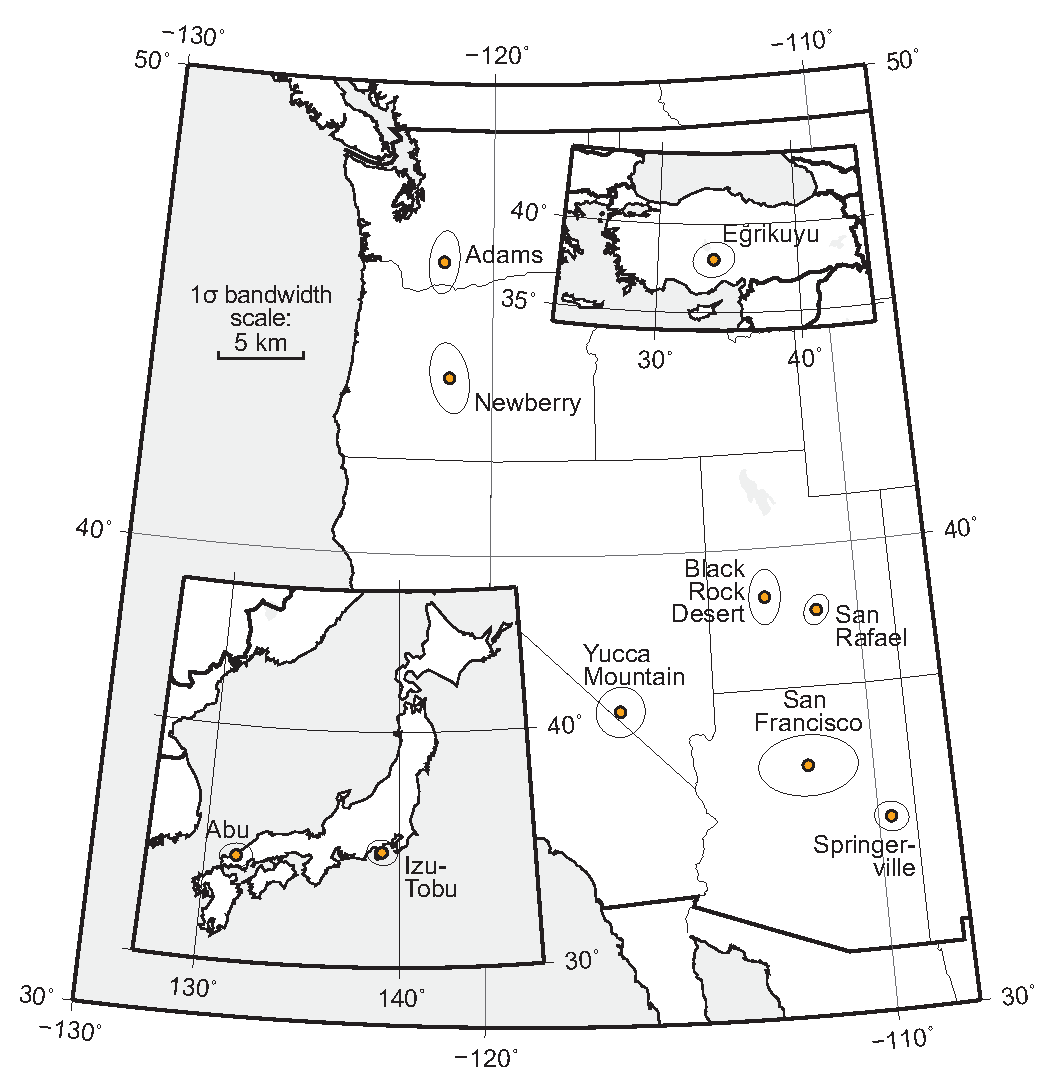
\includegraphics[width=0.5\linewidth]{\FigPath/locators/earth_locator.eps}
\caption{Locations of selected volcano clusters with their kernel bandwidth ellipses drawn over them. Ellipses are enlarged to show regional variation.}
\label{fig_earthlocator}
\end{figure}

\subsubsection{Earth clusters}
Ten distributed-style volcanic fields on earth have been mapped, producing vent catalogs that can be used to model vent density in the region. These clusters are located in four tectonic regimes: over subduction zones, on the Colorado Plateau, in the extensional Basin and Range region, and in the Anatolian Peninsula (Figure \ref{fig_earthlocator}).

\paragraph{Subduction-related clusters} 
Distributed volcanic fields in the Cascades Arc have formed in association with the large central volcanoes, including Mount Adams \citep{barron2014database} and Newberry Volcano \citep{bard2013database}. This arc is the product of the subducting Juan de Fuca plate. In southern Japan, monogenetic volcano groups have also formed, due to subduction of the Filipino and Pacific plates. Two of these volcano groups, the Abu Monogenetic Volcano Group and the Izu-Tobu Volcano Group have been mapped in this region \citep{kiyosugi2010relationships} and vent density has been modeled by \citet{kiyosugi2012relationship} Edifices in these catalogs are scoria cones, low shield volcanoes, and lava domes.

\paragraph{Colorado Plateau} Basaltic volcanism has occurred as an annulus around the Colorado Plateau during the Cenozoic \citep{tanaka1986migration}. Most of this volcanism has been distributed in nature, forming isolated volcano clusters. Three of these clusters, the San Francisco Volcanic Field (SFVF), Black Rock Desert, and the San Rafael Volcanic Field, are included in this study. 

Volcanoes in the SFVF, located in and around Flagstaff, AZ, have been mapped by \citet{harburger2014probabilistic}, including 583 vents identified as monogenetic. This field has been active for three magnetic epochs, enabling the field to be separated into three sub-fields which can be independently analyzed \citep{tanaka1986migration}. Black Rock Desert volcanoes in Utah were cataloged by \citet{hintz2008physical} and vent density has been modeled by \citet{kiyosugi2012relationship}. \citet{kiyosugi2012relationship} also mapped 126 conduits diatremes in the heavily eroded San Rafael Volcanic Field in central Utah and interpreted these to be previous vent locations when the field was active in the Pliocene.

\paragraph{Other tectonic settings} Two other vent databases have been created for clusters in the Basin and Range, Nevada, and in Central Anatolia, Turkey. In the Basin and Range, \citet{connor1995three} cataloged 39 scoria cones located in a cluster around Yucca Mountain. In Central Anatolia, \citet{uslular2015size} mapped 77 scoria cones, which form the E\u{g}rikuyu volcano cluster. The volume of each scoria cone is also reported by \citet{uslular2015size}.

\begin{figure}
\centering
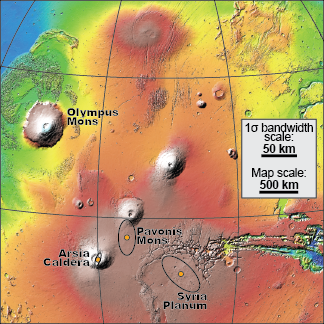
\includegraphics[width=0.5\linewidth]{\FigPath/locators/mars_locator_72dpi.png}
\caption{Locations of selected Martian volcano clusters in the Tharsis Volcanic Province. Kernel bandwidth ellipses are drawn at the 1$\sigma$ contour over them. Ellipses are enlarged.}
\label{fig_marslocator}
\end{figure}

\subsubsection{Mars clusters}
Three distributed-style volcanic fields within the larger Tharsis Province are included in this study: Syria Planum, Southern Pavonis Mons, and Arsia Mons Caldera. The Tharsis Volcanic Province has  been identified as a long lived center for volcanism since early space missions to Mars \citep{Carr1977} and makes up about one-quarter of the total global surface. Tharsis is home to many of the largest central-vent style volcanoes in the Solar System, but also has over 1,000 small volcanic vents that are distributed in clusters around Tharsis.

Three clusters of vents have been identified in the southern Tharsis region that are separated from other vents in the database and are treated as isolated populations because of this (Figure \ref{fig_marslocator}). Each field, Syria, Pavonis, and Arsia, were potentially formed from one magma generation event, though they might have also been formed from multiple events that created overlapping volcano clusters.

\paragraph{Southern Pavonis Mons}
Pavonis Mons is a large shield volcano in the Tharsis Montes, a linear chain of three shield volcanoes within the Tharsis Province. To the north and south of each of these volcanoes, lavas have been emplaced on the shield flank, apparently after the main construction phases of each shield \citep{bleacher2007tharsis}. These lavas are known as flank aprons \citep{bleacher2007tharsis}. At Pavonis, a volcano cluster of 88 shield volcanoes (one to tens km in diameter) is present on top of the southern flank apron \citep{bleacher2009spatial}. This cluster is aligned roughly N-S along the axis of the apron \citep{bleacher2009spatial}.


\paragraph{Arsia Mons Caldera}
Arsia Mons is the southernmost large shield volcano of the Tharsis Montes and has a 110~km diameter caldera at its summit. Within this caldera, 29 low shield volcanoes have been mapped [Chapter 4, this dissertation]. The caldera and shields within it are thought to be very young due to the absence of any impact craters larger than 1~km in the entire caldera \citep{crumpler1996calderas}. In addition to the 29 vent locations, volumes have been modeled for the lavas effused from each vent using an interpolated subsurface model for each lava flow [Chapter 4, this dissertation]. These volume estimates will be used to compare the spatial vent density of the field to a volume-weighted spatial density model.

\paragraph{Syria Planum}
The Syria Planum region is a broad plateau with 263 low shield volcanoes \citep{richardson2013volcanic}. One volcano, Syria Mons, has lava flows that travel up to 1,000~km from its vent \citep{baptista2008swarm}. The other low shields have been mapped by \citet{richardson2013volcanic} and are one to tens of km in diameter with slopes of $<6^{\circ}$. This volcano cluster has been dated using crater retention rate models to have formed between 3.6-2.9~Ga spanning the Hesperian geologic period on Mars.

\begin{figure}
\centering
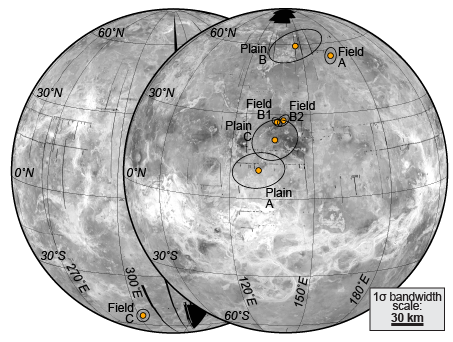
\includegraphics[width=0.6\linewidth]{\FigPath/locators/venus_globe_72dpi.png}
\caption{Locations of seven volcano clusters on Venus. Kernel bandwidth ellipses are drawn at the 1$\sigma$ contour over each cluster and are enlarged.}
\label{fig_venuslocator}
\end{figure}

\subsubsection{Venus clusters}
Seven Venus clusters have been cataloged by \citet{miller2012shield}, which fall into two distinct classes: four are ``shield fields'' which are composed of $10^3$-$10^4$ volcanic vents and three are ``shield plains'' which host $10^4$-$10^5$ volcanic vents (Figure \ref{fig_venuslocator}). Both types of cluster are formed by low sloped (less than one to a few degrees) shields $<$10~km in diameter \citep{richardson2012comparison}. These shields are radar bright or dark, enabling their mapping with left-look Magellan radar images, though their vents are often not visible, so vents are mapped as the centroid of the edifice \citep{miller2012shield}. Of the seven clusters cataloged, three are shield plains and four are shield fields \citep{miller2012shield}.

The large size difference between shield fields and shield plains has been observed since the return of Magellan radar images \citep{head1992venus}. Venusian shield fields are similar in size to the shield fields on Mars and have a similar number of vents (several hundreds) to fields on Mars and Earth. Venusian plains, however, are regional in scale and include several thousand vents. The Venusian surface has very few impact craters, indicating that it has recently been resurfaced. The regional volcanic plains would have played an important role in this resurfacing, due to their large footprints \citep{guest1992small}.

\begin{table}
\centering
\caption{Distributed-style Volcano Clusters}
\begin{tabular}{p{2cm} p{2.5cm} p{2cm} c c p{4cm}}
\toprule
Cluster	&	Region, &	Location	&	Vent &	Bandwidth	&	Data\\
Name		& Country	&	Lat, Long	&	Count	&	Matrix (km$^2$)	&Source\\
\midrule
Abu$^*$		&	Ch\={u}goku, Japan	&	34$^{\circ}$30'N, 131$^{\circ}$35'E	&	56	&	$\bigl[\begin{smallmatrix} 3.81&0.230\\0.230&2.05 \end{smallmatrix}\bigr]$	&	\citet{kiyosugi2012relationship,kiyosugi2010relationships}\\
Adams		&	Washington, USA	&	46$^{\circ}$10'N, 121$^{\circ}$30'W	&	89	&	$\bigl[\begin{smallmatrix} 3.25&0.989\\0.989&13.9 \end{smallmatrix}\bigr]$	&	\citet{barron2014database}\\
Blk. Rock Desert$^*$ &	Utah, USA		&	39$^{\circ}$N, 112$^{\circ}$30'W&	39	&	$\bigl[\begin{smallmatrix} 3.51&0.500\\0.500&10.6 \end{smallmatrix}\bigr]$	&	\citet{kiyosugi2012relationship,hintz2008physical}\\
E\u{g}rikuyu	&	Central Turkey	&	34$^{\circ}$N, 38$^{\circ}$E	&	77	&	$\bigl[\begin{smallmatrix} 10.8&1.00\\1.00&7.57 \end{smallmatrix}\bigr]$	&	\citet{uslular2015size}\\
Izu-Tobu$^*$	&	Ch\={u}bu, Japan	&	35$^{\circ}$N, 139$^{\circ}$20'E	&	126	&	$\bigl[\begin{smallmatrix} 3.29&-0.200\\-0.200&2.27 \end{smallmatrix}\bigr]$	&	\citet{kiyosugi2012relationship}\\
Newberry	&	Oregon, USA	&	43$^{\circ}$45'N, 121$^{\circ}$15'W	&	327	&	$\bigl[\begin{smallmatrix} 5.57&-2.43\\-2.43&17.3 \end{smallmatrix}\bigr]$	&	\citet{bard2013database}\\
San \mbox{Francisco}	&	Arizona, USA	&	35$^{\circ}$20'N, 111$^{\circ}$50'W	&	583	&	$\bigl[\begin{smallmatrix} 34.4&-0.0396\\-0.0396&13.0 \end{smallmatrix}\bigr]$	&	\citet{harburger2014probabilistic}\\
San Rafael	&	Utah, USA	&	38$^{\circ}$35'N, 111$^{\circ}$15'W	&	63	&	$\bigl[\begin{smallmatrix} 2.31&0.720\\0.720&3.12 \end{smallmatrix}\bigr]$	&	\citet{kiyosugi2012relationship}\\
Springerville &	Arizona, USA	&	34$^{\circ}$15'N, 109$^{\circ}$45'W	&	400	&	$\bigl[\begin{smallmatrix} 4.07&-0.300\\-0.300&3.14 \end{smallmatrix}\bigr]$	&	\citet{kiyosugi2012relationship,condit2010dynamic}\\
Yucca Mountain$^*$ &	Nevada, USA	&	36$^{\circ}$40'N, 116$^{\circ}$30'W	&	39	&	$\bigl[\begin{smallmatrix} 8.35&0.42\\0.42&8.75 \end{smallmatrix}\bigr]$	&	\citet{kiyosugi2012relationship,connor1995three}\\
Field-A	&	Atalanta, Venus	&	54$^{\circ}$N, 168$^{\circ}$E	&	344	&	$\bigl[\begin{smallmatrix} 115&7.74\\7.74&238 \end{smallmatrix}\bigr]$	&	\citet{miller2012shield}\\
Field-B1	&	Vellamo, Venus	&	27$^{\circ}$N, 137$^{\circ}$E	&	135	&	$\bigl[\begin{smallmatrix} 88.7&-35.4\\-35.4&71.4 \end{smallmatrix}\bigr]$	&	\citet{miller2012shield}\\
Field-B2	&	Vellamo, Venus	&	328$^{\circ}$N, 139$^{\circ}$E	&	169	&	$\bigl[\begin{smallmatrix} 125&51.7\\51.7&116 \end{smallmatrix}\bigr]$	&	\citet{miller2012shield}\\
Field-C	&	Mylitta, Venus	&	52$^{\circ}$S, 58$^{\circ}$W	&	290	&	$\bigl[\begin{smallmatrix} 140&2.93\\2.93&138 \end{smallmatrix}\bigr]$	&	\citet{miller2012shield}\\
Plain-A	&	Greenaway, Venus	&	11$^{\circ}$N, 130$^{\circ}$E	&	2919	&	$\bigl[\begin{smallmatrix} 2440&164\\164&1120 \end{smallmatrix}\bigr]$	&	\citet{miller2012shield}\\
Plain-B	&	Atalanta, Venus	&	60$^{\circ}$N, 150$^{\circ}$E	&	10225	&	$\bigl[\begin{smallmatrix} 2470&709\\709&1000 \end{smallmatrix}\bigr]$	&	\citet{miller2012shield}\\
Plain-C	&	Greenaway, Venus	&	20$^{\circ}$N, 135$^{\circ}$E	&	3460	&	$\bigl[\begin{smallmatrix} 1860&232\\232&1460 \end{smallmatrix}\bigr]$	&	\citet{miller2012shield}\\
Arsia		&	Tharsis, Mars	&	9$^{\circ}$S, 120$^{\circ}$W	&	29	&	$\bigl[\begin{smallmatrix} 81.4&105\\105&347 \end{smallmatrix}\bigr]$	&	Chapter X\\
Pavonis	&	Tharsis, Mars	&	4$^{\circ}$S, 114$^{\circ}$W	&	89	&	$\bigl[\begin{smallmatrix} 579&-0.616\\-0.616&2520 \end{smallmatrix}\bigr]$	&	\citet{bleacher2009spatial}\\
Syria		&	Tharsis, Mars	&	14$^{\circ}$S, 100$^{\circ}$W	&	263	&	$\bigl[\begin{smallmatrix} 2810&-1720\\-1720&2620 \end{smallmatrix}\bigr]$	&	\citet{richardson2013volcanic}\\
\bottomrule
\multicolumn{6}{p{0.95\linewidth}}{$^*$ Cluster data (including bandwidth matrix) are reported in \citet{kiyosugi2012relationship}, but vent locations are not included in this report.}\\
\label{tab_clusterdata}
\end{tabular}
\end{table}

\begin{table}
\centering
\caption{Sub-populations of the San Francisco Volcanic Field$^*$}
\begin{tabular}{l c p{2cm} c c}
\toprule
Magnetic	&	Time Span	& Centroid	&	Vent &	Bandwidth\\
chronozone		&	Ma	& Lat, Long	&	Count	&	Matrix (km$^2$)\\
\midrule
Brunhes	&	0.73 - Present	&	35$^{\circ}$20'N, 111$^{\circ}$30'W	&	239	&	$\bigl[\begin{smallmatrix} 21.6&-5.66\\-5.66&11.7 \end{smallmatrix}\bigr]$\\
Matuyama	&	2.48 - 0.73	&	36$^{\circ}$20'N, 112$^{\circ}$W	&	209	&	$\bigl[\begin{smallmatrix} 15.0&1.38\\1.38&25.4 \end{smallmatrix}\bigr]$\\
Pre-Matuyama	&	5-2.48	&	36$^{\circ}$20'N, 112$^{\circ}$15'W	&	135	&	$\bigl[\begin{smallmatrix} 13.3&-3.10\\-3.10&12.5 \end{smallmatrix}\bigr]$\\
\midrule
Entire Field	&	5 - Present	&	35$^{\circ}$20'N, 111$^{\circ}$50'W	&	583	&	$\bigl[\begin{smallmatrix} 34.4&-0.0396\\-0.0396&13.0 \end{smallmatrix}\bigr]$\\
\bottomrule
\multicolumn{5}{p{0.95\linewidth}}{$^*$Vent locations reported in \citet{harburger2014probabilistic}.}\\
\label{tab_sfvfdata}
\end{tabular}
\end{table}

\subsection{Estimating vent density with the KDtools Python Library}

A python library has been created to map the spatial density of geographic points, with specific functions to deal with geographic projections on Earth, Mars, and Venus. This library, called KDtools, contains seven functions which can be used to pre-process data, identify an optimal kernel bandwidth of the data, evaluate the local point density for locations on a map, and export these results to a raster file. Each function is given in an appendix below (Section \ref{sec_kdtoolscode}). Two functions, explained below, are used to first identify an optimal kernel bandwidth and second evaluate the spatial density of points across a map grid.

The kernel bandwidth is determined with the SAMSE method in the \textbf{samse\_bandwidth} function, by calling the R statistical language in which the SAMSE bandwidth selector has been programmed. The single input of this function is the list of locations of each volcanic vents projected in meter units. A $2\times 2$, unconstrained covariance matrix is returned from this function.

Local vent density is calculated along a grid in the function \textbf{KD} with the covariance matrix defining the Gaussian kernel ellipse. The smoothed density of each vent is calculated over the grid locations given their distance from the vent. This density is then added to the total density at each location in order to form the summation shown in Equation \ref{eq_kde}. After the density functions attributed to all vents have been calculated over the grid, all density values are normalized with the left half of Equation \ref{eq_kde}. The output of this function is a 2-dimensional array of density values corresponding to the grid surrounding vent locations. The sum of these density values approaches 1.0 as the grid size is increased around the volcano cluster. Volume density can also be modeled with function \textbf{KD} by providing weights to the function, following Equation \ref{eq_weigthedkde}.

\section{Results}
The locations, vent counts, and kernel bandwidth matrices for each volcano cluster are reported in Table \ref{tab_clusterdata}. Data and results for four clusters, Abu Monogenetic Volcano Group, Izu-Tobu Monogenetic Volcano Group, Black Rock Desert, and the Yucca Mountain Volcano Group are duplicated in Table \ref{tab_clusterdata} from \citet{kiyosugi2012relationship}. In addition to modeling vent density for the entire field, vent density is modeled for each paleomagnetic sub-group in the San Francisco Volcanic Field. Vent count and bandwidth matrices are listed separately in Table \ref{tab_sfvfdata}.

\begin{figure}
\centering
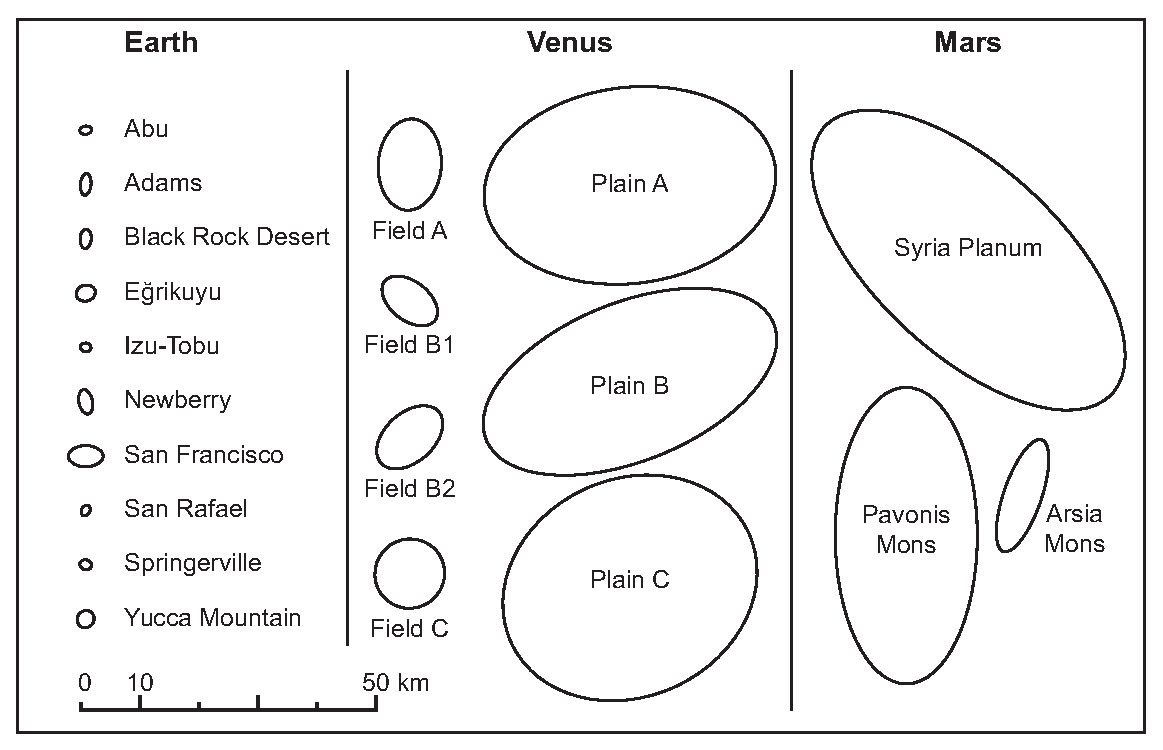
\includegraphics[width=0.7\linewidth]{\FigPath/Kernel-Ellipses.eps}
\caption{Kernel bandwidth ellipses for different clusters on Earth, Venus, and Mars. Each ellipse is drawn to scale, representing the 1$\sigma$ contour of the Gaussian bandwidths. The tightest bandwidths correspond to Earth clusters, while the broadest bandwidths correspond to Venus shield plains and Martian clusters.}
\label{fig_bandwidths}
\end{figure}

Because each bandwidth covariance matrix describes a bivariate normal distribution (Equation \ref{eq_covariance}), each bandwidth can be visualized as an ellipse drawn at a contour of the normal distribution. At the $1\sigma$ contour, the ellipse width in the x-direction is the square root of the top left number of the covariance matrix and the height is the square root of the bottom right number. Ellipses have been drawn for each cluster with the \textbf{ellipseGen} function in the KDtools library and are illustrated over each cluster location in Figures \ref{fig_earthlocator}, \ref{fig_marslocator}, and \ref{fig_venuslocator}. All bandwidth ellipses are also drawn to the same scale on Figure \ref{fig_bandwidths}. The sizes of bandwidths radically change by planet. The smallest bandwidths calculated are all for clusters on Earth. Mars and Venus both have large and small bandwidths. The two bandwidth sizes for Venus clusters indicate cluster type: shield fields have tighter bandwidths than shield plains.
%talk more about the bandwidths or, just talk about size of fields.

Bandwidths selected for each volcano cluster are then used to model the spatial density of volcanic vents in the cluster. These density models are mapped in several following figures. While the boundary of a volcanic field is often difficult to determine, spatial density models can be used to define a cluster area. Here, cluster area will be defined as the area within a spatial density contour that contains 95\% (2$\sigma$) of the cumulative spatial density. In other words, the area within the given contour contains 95\% of the probability of a new vent being created in the cluster, if the area is still volcanically active. The average spatial vent density is calculated by dividing the number of vents in the contour by the area within the contour. Cluster area and mean vent density are reported for each cluster in Table \ref{tab_results}.

\begin{table}
\centering
\caption{Size and Mean Vent Density of Volcano Clusters}
\begin{tabular}{l l c c c}
\toprule
& & 2-$\sigma$ Cluster & Vent Count in	&	Mean Vent\\
Field	&	Location & Area & Cluster Area	&	Density\\
\midrule
Adams	&	USA	&	1090	km$^2$	&	89 &	8.17$\cdot10^{-2}$ vents~km$^{-2}$	\\
Egrikuyu	&	Turkey	&	1009 &	77	&	7.63$\cdot10^{-2}$	\\
Newberry	&	USA	&	1760	&	326	&	1.85$\cdot10^{-1}$	\\
San Francisco	&	USA	&	5440	&	583	&	1.07$\cdot10^{-1}$	\\
San Rafael	&	USA	&	916	&	63	&	6.88$\cdot10^{-2}$	\\
Springerville	&	USA	&	2430	&	393	&	1.62$\cdot10^{-1}$	\\
Field-A	&	Venus	&	31800	&	341	&	1.07$\cdot10^{-2}$	\\
Field-B1	&	Venus	&	8890	&	134	&	1.51$\cdot10^{-2}$	\\
Field-B2	&	Venus	&	14600	&	168	&	1.15$\cdot10^{-2}$	\\
Field-C	&	Venus	&	19100	&	289	&	1.51$\cdot10^{-2}$	\\
Plain-A	&	Venus	&	1050000	&	2873	&	2.74$\cdot10^{-3}$	\\
Plain-B	&	Venus	&	1460000	&	10016	&	6.86$\cdot10^{-3}$	\\
Plain-C	&	Venus	&	986000	&	3397	&	3.45$\cdot10^{-3}$	\\
Arsia	&	Mars	&	10300	&	29	&	2.82$\cdot10^{-3}$	\\
Pavonis	&	Mars	&	118000	&	89	&	7.54$\cdot10^{-4}$	\\
Syria	&	Mars	&	325000	&	260	&	8.00$\cdot10^{-4}$	\\
\bottomrule
\label{tab_results}
\end{tabular}
\end{table}

%comparison
The sizes and quantities of vents of clusters in Table \ref{tab_results} are also charted in Figure \ref{fig_ventdens}. This illustrates significant differences between the cluster area and vent densities of different planets and cluster types. Distributed-style volcanic fields on Mars, Earth, and shield fields on Venus all have a similar population range of tens to several hundred vents. Venus shield plains are unique in that they have thousands to over ten-thousand vents associated with the same cluster. Earth fields sizes appear to cluster on the order of 10$^3$~km$^2$. Venus shield fields are an order of magnitude more spacious, with sizes on the order of 10$^4$~km$^2$. The Arsia Mons field on Mars is also this size, while the other two Mars fields, Pavonis and Syria, have footprints an order of magnitude larger yet at 10$^5$~km$^2$. The largest clusters are the Venus shield plains, which also have the most vents, having footprints on the order of 10$^6$~km$^2$.

Each planet also has a characteristic range of vent density (Table \ref{tab_results}. Earth clusters have 10$^{-1}$-10$^{-2}$ vents~km$^{-2}$, Venus clusters have 10$^{-2}$-10$^{-3}$ vents~km$^{-2}$, and Mars clusters have 10$^{-3}$-10$^{-4}$ vents~km$^{-2}$. Figure \ref{fig_ventdens} is contoured by three orders of magnitude of vent density, where there are 10, 100, and 1,000 km$^2$ within the defined cluster area per mapped volcanic vent. This shows that vent count and cluster size are correlated at the planetary scale.

\begin{figure}[h!]
	\centering
	\begin{gnuplot}[terminal=latex, terminaloptions=rotate]
		unset key
		set size 1,1
		set logscale xy 10
		set xlabel "Vent count in volcano cluster" rotate by 90
		set ylabel "2-$\sigma$ Cluster Size (km$^2$)"
		set xrange [20:12000]
		set yrange [500:4e6]
		set label "10 km$^2$ per vent" at first 1500, first 1e4 rotate by 23
		set label "100 km$^2$ per vent" at first 1500, first 1e5 rotate by 23
		set label "1000 km$^2$ per vent" at first 600, first 4e5 rotate by 23
		plot "ventdens_model.dat" using 1:2 with lines lt 4,\
		"ventdens_model.dat" using 1:3 with lines lt 4,\
		"ventdens_model.dat" using 1:4 with lines lt 4,\
		"ventdens_earth.dat" using 1:2 with points pt 6,\
		"ventdens_venus.dat" using 1:2 with points pt 7,\
		"ventdens_mars.dat" using 1:2 with points pt 3
	\end{gnuplot}
	\caption{Cluster size, defined by the area within the 2-$\sigma$ contour of vent density of each cluster, plotted with respect to the number of vents in the cluster. Earth clusters are drawn as hollow circles, Venus clusters are drawn as solid circles, and Mars clusters are asterisks. Three contours are drawn as dotted lines to show cluster size if there were 10, 100, or 1000 km$^2$ in the cluster area per volcanic vent.}
	\label{fig_ventdens}
\end{figure}
	

\subsection{Volume Flux Density}
Using KDE, vent density of several volcano clusters have been modeled with the implication that the probability of a new vent forming in the cluster is spatially constrained by these density models. In addition to this application, vents have been weighted by erupted volume to model the relative volume flux over the field. Mapping volume density (km$^3$~km$^-2$) can be an important tool to identify regions in a volcanic field where eruptions are disproportionally larger than those in other regions of the field.

\citet{uslular2015size} mapped 77 scoria cones in the E\u{g}rikuyu volcano cluster (Turkey) and provided the volumes for each cone. This enables both the vent density and the erupted volume density to be mapped. Figure \ref{fig_egrikuyu_kdevol} illustrates the two density models. On the left of Figure \ref{fig_egrikuyu_kdevol}, vents are weighted equally producing a vent density model that has a large sub-cluster of densely packed vents in the western half of the vent population though there is also a small cluster of vents packed at a similar density in the far east of the vent population. When vents are weighted by volume, as shown on the right of Figure \ref{fig_egrikuyu_kdevol}, the eastern mode disappears because the large amount of vents to the east are small in volume compared to the vents in the western mode of vents.

\begin{figure}[h!]
    \centering
    \begin{subfigure}{0.49\textwidth}
        \centering
        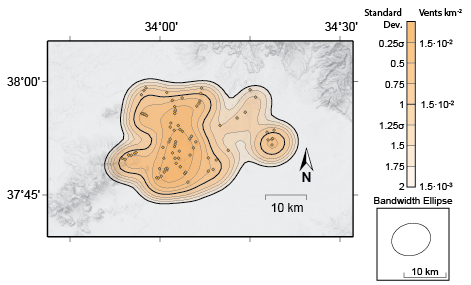
\includegraphics[width=\linewidth]{\FigPath/egrikuyu_kde_72dpi}
    \end{subfigure} 
    \begin{subfigure}{0.49\textwidth}
        \centering
        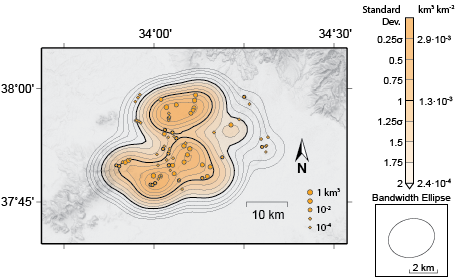
\includegraphics[width=\linewidth]{\FigPath/egrikuyu_vol_72dpi}
    \end{subfigure}
    \caption{Left, vent density of the E\u{g}rikuyu volcano cluster, Turkey. Right, erupted volume density. While a large number of vents in the eastern margin of the field make a second mode of vent density, their cumulative erupted volume is much smaller than the volumes erupted from vents in the center of the cluster, so the eastern mode is not seen in the volume density model.}
\label{fig_egrikuyu_kdevol}
\end{figure}

The lava flows that make up the distributed vent field in the Arsia Mons Caldera on Mars also have modeled volumes that correspond to each eruptive event. Figure \ref{fig_arsia_kdevol} shows both the vent density plot of the vent field and the modeled volume distribution. Similar to the E\u{g}rikuyu field, this shows the difference in vent productivity, where the eastern half of the field has vents which produced larger eruptions than the western vents.

\begin{figure}[h!]
    \centering
    \begin{subfigure}{0.49\textwidth}
        \centering
        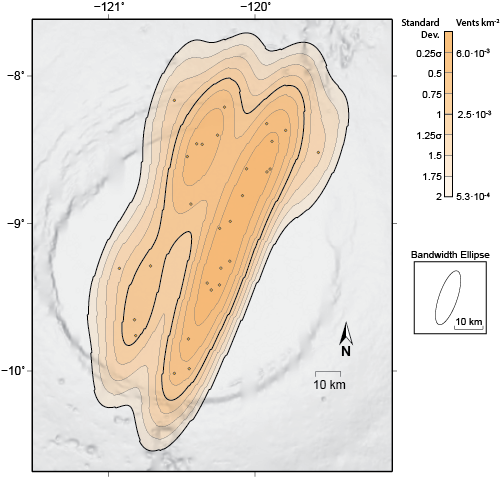
\includegraphics[height=8cm]{\FigPath/arsia_kde_72dpi}
    \end{subfigure} 
    \begin{subfigure}{0.49\textwidth}
        \centering
        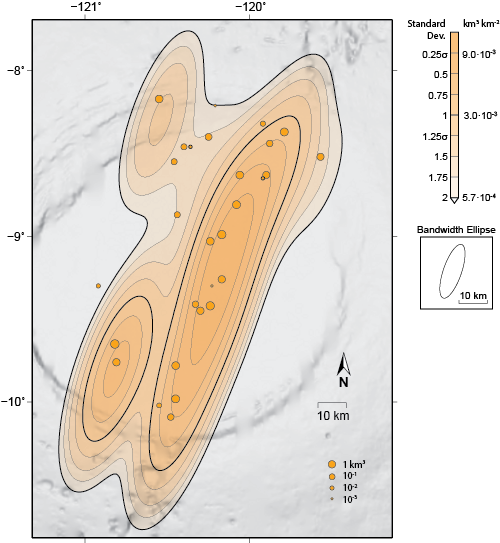
\includegraphics[height=8cm]{\FigPath/arsia_vol_72dpi}
    \end{subfigure}
    \caption{Left, vent density of the Arsia Mons Caldera volcanic field (Mars). Right, erupted volume density using minimum volume estimates made using interpolated subsurface models for each volcano. The volume density plot shows that lavas from the east lineament of vents, also visible in the vent density model, are more voluminous than those from the east lineament of vents.}
\label{fig_arsia_kdevol}
\end{figure}

\section{Discussion}
The major finding of this study is that the spatial density of vents between planets is generally different by an order of magnitude. On Earth, six monogenetic volcano clusters are shown to all cluster on the order of 0.1 vents per km$^2$. On Mars, two clusters have a vent density of around 0.001 vents per km$^2$. One cluster, in the basaltic caldera of Arsia Mons, is more focused by a factor of five. In between these vent densities, Venus shield fields have densities of 0.01 vent per km$^2$. Venus shield fields are still more focused than the regional shield plains, which have an average density of 0.003 vents per km$^2$, similar to the Arsia Mons cluster. Essentially, volcanic vents in Earth fields have 10s km$^2$ of space between neighboring vents, on Venus, distributed volcanoes have 100s km$^2$ of individual space, and on Mars, two of three fields have 1000s  km$^2$ of space between neighboring vents, while one is clustered on a ``Venusian'' scale.

\subsection{Geologic implications of the kernel bandwidth}
Each bandwidth ellipse mimicseparatelys attributes of its corresponding vent cluster and likely reflects geologic properties which effect the volcano cluster. The bandwidth ellipse area at one standard deviation (1-sigma) reflects both the spatial extent of volcanoes in the cluster and the number of vents in the cluster. Larger volcano clusters correlate with larger bandwidths ellipses, while clusters with more volcanoes in the same amount of space have smaller bandwidths. Because bandwidth area is correlated with these two characteristics, it is better to refer to each characteristic directly. Similarly, bandwidth ellipse elongation, or the difference in the major and minor axis standard deviations, is a function of the anisotropy in vent production through the cluster, either because of a farther extent of volcanoes in one direction or because of more vents per km in one direction. Because of this, the anisotropy of vent production in a cluster can be explored using bandwidth elongation as a proxy.

Elongation of the bandwidth of a volcano cluster can be explained by one or a combination of at least three geologic processes. First, the magma source region underlying the volcano cluster might be elongated, matching the distribution of volcanoes observed at the planet's surface. Second, the magma source region might have migrated with time or multiple magma source regions that are spatially adjacent might be overprinting pre-existing populations. Third, the hydraulic conductivity of the crust might itself be anisotropic, preferentially focusing magma in one direction or enabling magma to spread laterally away from a source region. While all three of these might apply to all volcanic fields in varying degrees of magnitude, I will discuss how the anisotropy seen in the bandwidth ellipse might be explained by one of these processes for example clusters. Comparing bandwidth orientation and elongation to different magmatic and tectonic processes might help explain the relative power different processes have in governing the shape of volcano clusters in different regions.

\begin{figure}
\centering
\begin{subfigure}{0.49\textwidth}
\centering
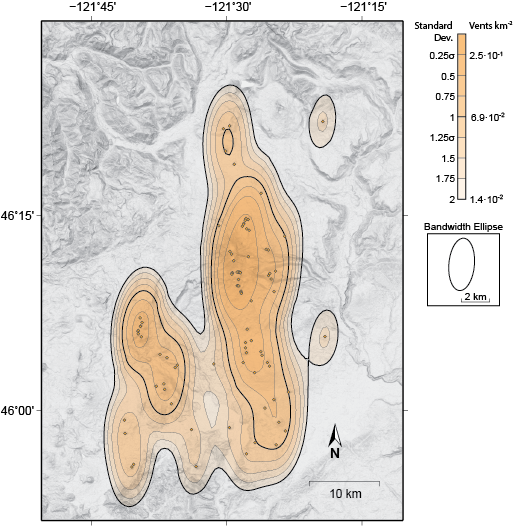
\includegraphics[width=\linewidth]{\FigPath/adams_kde_72dpi}
\end{subfigure}
\begin{subfigure}{0.49\textwidth}
\centering
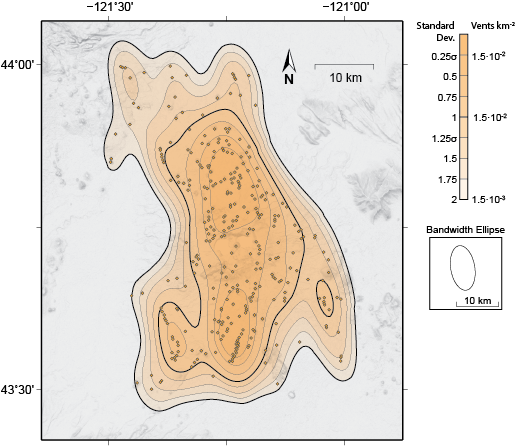
\includegraphics[width=\linewidth]{\FigPath/newberry_kde_72dpi}
\end{subfigure}
\caption{Volcanic vent density of monogenetic volcanoes near (left) Mt. Adams (Washington, USA) and (right) Newberry Volcano (Oregon, USA). If the magma source region is elongated N-S due to the subduction of the Juan de Fuca Plate to the west, this might result in an elongated volcano distribution and kernel bandwidth ellipse.}
\label{fig_adams-newbkde}
\end{figure}

\subsubsection{Elongated Source Region}
The bandwidth ellipse of elongated clusters is often elongated in the same direction, such as the ellipse for scoria cones around Mount Adams, Washington (left, Figure \ref{fig_adams-newbkde}). The distributed volcanic field around Mount Adams runs parallel to the Cascades volcanic arc, possibly because the magma source region of the field runs along the axis of the Arc. As can be seen in Figure \ref{fig_earthlocator}}, both Cascades clusters, Adams and Newberry, have kernel bandwidths that are in line with the volcanic arc (Figure \ref{fig_adams-newbkde}). Both Japanese clusters, Abu and Izu-Tobu, also have bandwidths in line with the arc that makes the lower limb of the country's main island, Honshu. For regions where magmatic activity is expected to be elongated, it is possible that bandwidth ellipse orientation is primarily due to the elongation of the magma source region.



\subsubsection{Magma source migration or multiple overprinting sources}
The eastward migration of volcanism in the San Francisco Volcanic Field is observed from paleomagnetics. The volcano cluster has been active for three magnetic epochs. The most recent volcanoes, including the $\sim$1000 year old Sunset Crater, are located in the eastern portion of the field and were emplaced during a normal-polarity magnetic field \citep{tanaka1986migration}. Volcanic edifices with reverse polarity in this field are located in the center of the field. The oldest volcanoes are to the west and are normally magnetized again. \citet{tanaka1986migration} labeled the most recent sub-group the Brunhes group, the reverse-magnetized sub-group the Matuyama group, and the oldest group the pre-Matuyama group. If the geographic centroid of each group is located, an eastward (93$^{\circ}$N) march of the sub-group centroids of 2.9$\pm$0.3 cm/yr can be observed \citep{tanaka1986migration}.

\begin{figure}
\centering
\begin{subfigure}{0.49\textwidth}
\centering
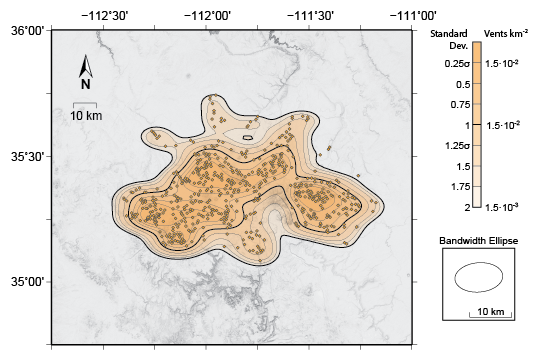
\includegraphics[width=\linewidth]{\FigPath/sanfrancisco_kde_72dpi.png}
\end{subfigure}
\begin{subfigure}{0.49\textwidth}
\centering
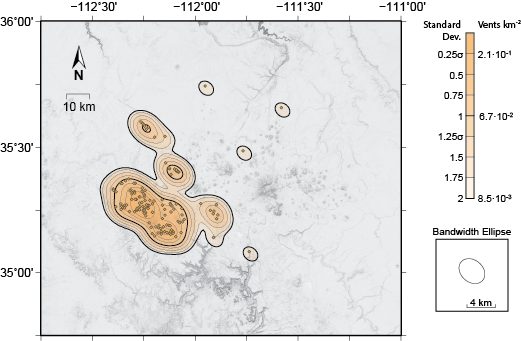
\includegraphics[width=\linewidth]{\FigPath/sanfranciscoP_kde_72dpi.png}
\end{subfigure}
\begin{subfigure}{0.49\textwidth}
\centering
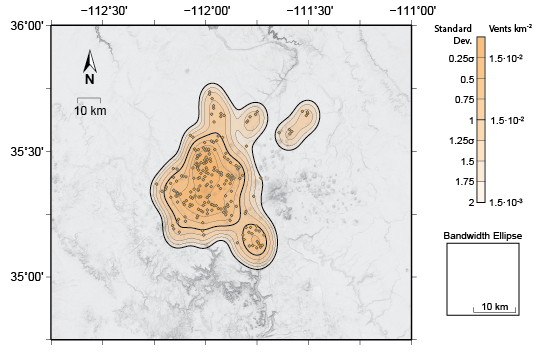
\includegraphics[width=\linewidth]{\FigPath/sanfranciscoM_kde_72dpi.png}
\end{subfigure}
\begin{subfigure}{0.49\textwidth}
\centering
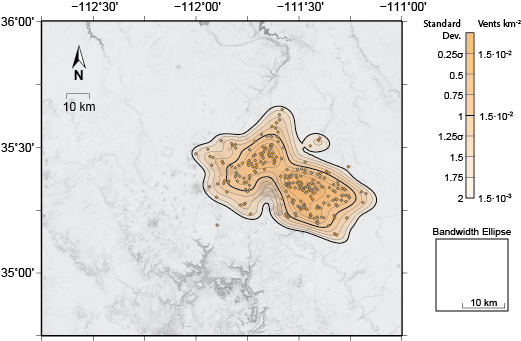
\includegraphics[width=\linewidth]{\FigPath/sanfranciscoB_kde_72dpi.png}
\end{subfigure}
\caption{Vent density through time for the San Francisco Volcanic Field (Arizona, USA). Top left, the entire volcanic field including 583 vents. Top right, spatial density of vents created during the Pre-Matuyama magnetic chronozone, 5-2.48~Ma \citep{tanaka1986migration}. Bottom left, density of Matuyama-age, 2.48-0.73~Ma vents. Bottom right, Bruhnes-age, 0.73-present, activity. While volcanic activity has migrated eastward, the kernel bandwidth ellipse has also changed. Taking all age vents into account, the bandwidth ellipse is oriented in the direction of migration (top right).}
\label{fig_sfvfkde}
\end{figure}

This eastward march can be compared to the modeled kernel bandwidths of each volcano sub-group (Figure \ref{fig_sfvfkde}). None of the three subgroups' bandwidths are elongated in the direction of the migration identified by \citet{tanaka1986migration}. Bandwidth ellipses of two of the subgroups, the pre-Matuyama and the current Brunhes are elongated in to the northwest, possibly in line with a pre-existing NW-SE fracture set that heavily influences vent geometry  in the field \citep{marshall2015subsurface}. However, the bandwidth ellipse calculated for the entire field is in line with this migration.

Similarly, formation of scoria cones in the Springerville volcanic field is seen to migrate in an ESE direction, 106$^{\circ}$, by 2.5$\pm$0.8 cm/yr. Unlike the San Francisco Volcanic Field, this field is not divided by magnetic epochs, but the group has been divided into two units, older and younger than 1.2~Ma, using K-AR dating and stratigraphy by \citet{condit1989patterns}. Similar to \citet{tanaka1986migration}, the centroids of the two units, together comprised of 230 scoria cones, are used to calculate the velocity of the migration. Like the San Francisco Volcanic Field, the bandwidth ellipse is elongated in the direction of the migration, though not as noticeably as the former.

On Mars, volcanic activity on Syria Planum also migrated over the course of its development. \citet{richardson2013volcanic} identified two major sub-clusters of coalesced shield volcanoes, separated by a large lava flow front of one of the clusters, which embayed volcanoes of the other cluster. The embayment suggests that the southeast group of volcanoes was emplaced first, with crater age-date modeling suggesting an age of 3.4-3.2~Ga. The northwest group was then emplaced between 3.2-2.6~Ga \citep{richardson2013volcanic}. Because of the high uncertainty currently associated with crater age-dating, it is possible that the entire field was emplaced without a migration from the southeast to the northwest. In this case, the bandwidth ellipse (Figure \ref{fig_syriakde}) might be more indicative of the geometry of the magma source region. If, however, there was a migration of magmatic activity or if the two clusters are simply two magmatic events that occured in the same location, the elongation of the bandwidth ellipse would be explained by this migration.

\begin{figure}
\centering
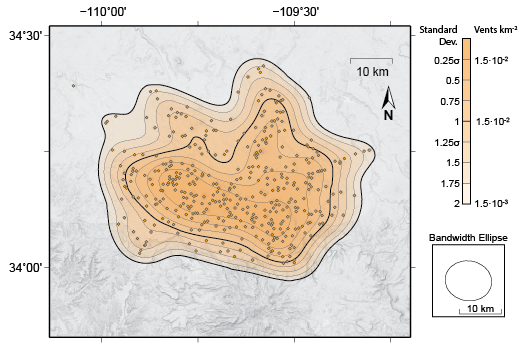
\includegraphics[width=0.6\linewidth]{\FigPath/springerville_kde_72dpi}
\caption{Volcanic vent density of the Springerville Monogenetic Volcanic Field (Arizona, USA). The migration of the magma source with respect to the crust over time might be the source of the E-W elongated kernel ellipse.}
\label{fig_springervillekde}
\end{figure}

\begin{figure}
\centering
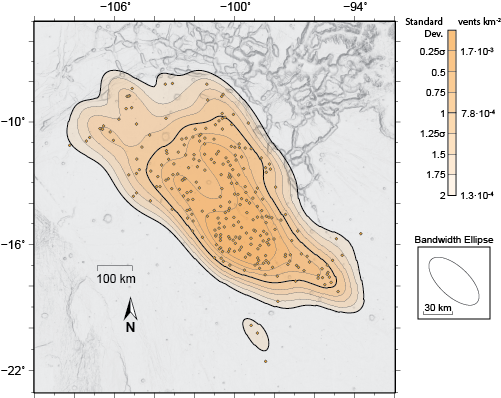
\includegraphics[width=0.6\linewidth]{\FigPath/syria_kde_72dpi}
\caption{Spatial vent density model of Syria Planum, Mars. A northwest migrating magma source or two overprinting magma sources to the northwest and southeast might explain the elongation of the field.}
\label{fig_syriakde}
\end{figure}


\subsubsection{Anisotropic crustal conductivity}
\citet{bonafede1998porous} modeled the crust under Mount Etna as a porous medium through which pressurized magma can freely flow. In this model, magma migrates based on a hydraulic head pressure and the hydraulic conductivity of the crust. If conductivity is low, magma will flow less, while if conductivity is high, magma will flow more easily through the medium. By modeling an anisotropic conductivity, where conductivity is less or more for magma traveling east or west than for magma traveling north or south, \citet{bonafede1998porous} were able to match the expected surface output of magma to the historical distribution of flank eruptions at Etna. 

Hydraulic conductivity in the crust can be related to pre-existing fracture sets, as aligned fractures enable magma to propagate more easily in the direction parallel to the fractures. Conductivity can also be a product of dynamic stress, since dikes open in the direction of least compressive stress and propagate in directions normal to the least compressive stress. 

If magma can propagate easily in one direction, but not in another direction, then magma will be less focused in the direction of lateral propagation. Were the magma source region a point at depth, then the shape of the field might solely be a product of this anisotropic conductivity in the lithosphere. Because the elliptical bandwidth can be used as a proxy for field elongation, directional conductivity differences can potentially be identified by comparing the bandwidth orientation to the direction of geologic features that would increase or decrease lithospheric conductivity (e.g. direction of crustal strain, pre-existing joints, graben). 

\begin{figure}
\centering
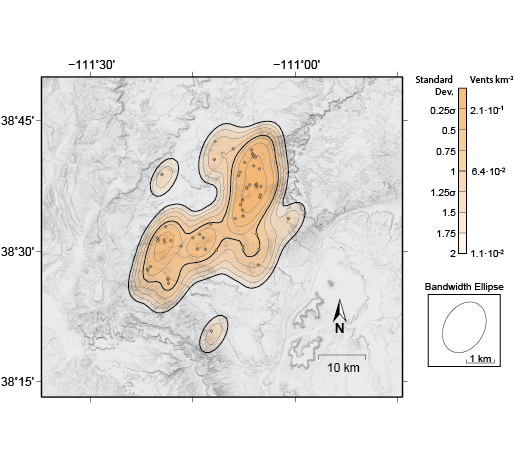
\includegraphics[width=0.6\linewidth]{\FigPath/sanrafael_kde_72dpi}
\caption{Volcanic conduit density of the San Rafael Volcanic Field (Utah, USA). Dikes are oriented north following pre-existing joint sets in the upper crust, possibly influencing the shape of the kernel ellipse.}
\label{fig_sanrafaelkde}
\end{figure}

The San Rafael volcanic field is one example where existing crustal features likely play a significant role in the overall distribution of volcanic vents. The San Rafael Swell has been eroded in the Holocene to expose the magma plumbing system of the volcanic field \citep{richardson2015sills}. Conduits which formed volcanoes in this field are mapped in Figure \ref{fig_sanrafaelkde} and are located along dikes as locations where a dike widened to create conduit diatreme. Dikes in this field are oriented N15W to N, and were likely oriented in this direction by well-developed joints in the Glen Canyon Group: sedimentary rocks underlying the field \citep{delaney1997physical}. The elliptical bandwidth orientation in this field is 30$^{\circ}$N (Figure \ref{fig_sanrafaelkde}), which is not perfectly in line with the dike orientation. However, it is possible that the primary N-S elongation of this bandwidth is due to the joint orientation, while the E-W component can be explained by some other process (e.g. source region geometry).


\begin{figure}
\centering
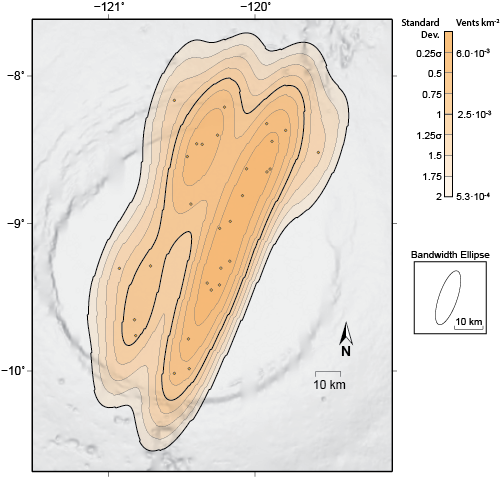
\includegraphics[width=0.6\linewidth]{\FigPath/arsia_kde_72dpi}
\caption{Volcanic vent density of the Arsia Mons Caldera Volcanic Field (Mars). Each root of the tooth-shaped density model is parallel with large rift graben that cut the flanks of the volcano.}
\label{fig_arsiakde}
\end{figure}

On Mars, the volcanic field in the Arsia Mons Caldera is also likely shaped by pre-existing fractures in the volcano. Arsia Mons is located at the southern end of the Tharsis Montes and is cut by two large sets of grabens. These grabens are visible on the upper flanks of the mountain but are not visible in the 110~km caldera of Arsia. Instead the caldera is covered by young lava flows that were emplaced from 29 volcanic vents, mapped in Figure \ref{fig_arsiakde}. The density model of the Arsia field is bimodal with two long, parallel lineaments of vents spanning the diameter of the caldera. The orientation of the bandwidth major axis is 19$^{\circ}$N, which is also the orientation of the two graben sets. In addition to this, the two lineaments of vents in Figure \ref{fig_arsiakde} are each in line with one of the rift graben. This is evidence that the dikes that created this vent field would have preferentially ascended parallel to the existing faults.

\section{Conclusions}
The spatial density of volcanic vents in distributed volcano clusters on three different planets has been modeled using Kernel Density Estimation. Vent density for clusters appears to be governed on the planetary scale, with vent density being highest at Earth clusters, lowest at Mars clusters, and intermediate in Venus clusters. While most clusters have tens to hundreds of vents, Venus shield plains have thousands of vents. Shield plains are also the largest clusters by area, but have similar vent density (0.001 vents per km$^2$) as the shield fields on Venus.

The kernel bandwidths of volcano clusters, or the bivariate normal distributions used to model spatial density, have been calculated using the SAMSE selector \citep{duong2007}, which estimates the bandwidth size assuming the distribution of point features on a map is a random sample of an unknown 2D probability density function. These bandwidths, like the size and vent density of clusters, also are unique to each planet. 

Bandwidth orientation and elongation might also be indicative of underlying characteristics of the lithosphere or the magma source region itself. Three possible processes might influence bandwidth dimensions: an elongated source region, source region migration, and anisotropic conductivity in the crust that enables or inhibits magma focusing in different directions. While a kernel bandwidth and its corresponding volcano cluster might be influenced by any or all three of these processes, the relative amount that each of these processes influences the cluster formation can be estimated by comparing the bandwidth orientation to hypothesized or known features of the underlying magmatic and tectonic systems.


%\addcontentsline{toc}{section}{References}
%\bibliographystyle{plainnat}
%\bibliography{kde}

%%%%%%%%%%%%%%%%%%%%%
%References Section
\section{References}
\bibliography{kde}
\bibliographystyle{apalike} 

\section{Appendix: KDtools}
\label{sec_kdtoolscode}
Below are the functions as written in the kdtools python library. This library is available on github at \url{https://github.com/jarichardson/kdtools}.

\subsection{contourBySigma}
\begin{verbatim}
def contourBySigma(Z, 
  sigmas=[0.25,0.5,0.75,1.0,1.25,1.5,1.75,2.0,2.25,2.5,2.75,3.0],
  gridspacings=[1,1]):
  '''
  Identifies Density contour levels given Sigma thresholds.
  Contours define areas within which lay X% of the total field density
  e.g.: Within the Sigma-2.0 contour lies 95.4% of total field density.
        The density value of each contour decreases with increasing
        sigma.
  Requires a numpy array of density values (Z), with any shape.
  Optionally, provide a list of requested sigma thresholds, and the
  grid size as a 2 item list, to normalize the density.
  
  Outputs a dictionary of {sigma-level: density value}. If sigma-levels
  are not found (off the grid if the grid is too small), they will not
  be included in the dictionary.
  '''
  #find cumulative density that is used to pass the given
  #sigma thresholds in "contours"
  cum_thresholds = 2*(norm.cdf(sigmas)-norm.cdf(0))
  
  integrate = 0.0
  curcontour = 0
  densitycontours = {}
  
  #sort and reverse Z
  Z = numpy.sort(Z,kind='quicksort',axis=None)[::-1]
  
  #assuming density units are m^-2, but spacing is not 1 cell m^-2
  #reduce cumulative threshold by grid resolution
  cum_thresholds *= 1.0/(gridspacings[0]*gridspacings[1])
  
  for i,d in enumerate(Z):
    integrate+=d
    #if the elapsed density surpasses the next contour
    if (integrate >= cum_thresholds[curcontour]):
      densitycontours[sigmas[curcontour]] = d
      curcontour += 1
      if (curcontour>=len(sigmas)):
        break
  
  return densitycontours
\end{verbatim}

\subsection{densityToRaster}
\begin{verbatim}
def densityToRaster(griddata, ranges, spacings, outrastername, clon=-999, 
  utmzone=-999, planet='earth', driver='GTiff', outproj="tm"):
  '''
  Outputs a 2-D array to a gdal-readable raster. Input expected to be
  in a transverse mercator projection.
  griddata: 2D data array
  outrastername: file name of raster output. If meter output is desired,
     it would be good practice to define clon or utm zone
  planet: 'earth','venus', or 'mars'. This is only needed to translate to
     latlong projections
  clon: center longitude of non-earth transverse mercator data
  utmzone: utm zone of earth data
  driver: gdal-readable raster short name [GTiff]
  outproj: 'tm' or 'll' for transverse mercator (no tranformation occurs)
     or latlong (gdalwarp will be implemented). [tm]
     
  ISSUES: If values are very low (normal for density grids), gdalwarp 
       doesn't work, so it is suggested that output remain in meters.
       A workaround might be to supply log10 values of griddata.
  '''
  
  #print an extra line for good looks
  print ""
  
  #Check that the user's requested driver will actually work before
  #doing anything
  userdriver = gdal.GetDriverByName(driver)
  if userdriver==None:
    print '\nerror: Raster type "'+driver+'" not a valid gdal driver!'
    print '  No map created.'
    return None
  
  gdaldriver = gdal.GetDriverByName('GTiff')
  gdaldriver.Register()
  cols = numpy.shape(griddata)[1]
  rows = numpy.shape(griddata)[0]
  bands = 1
  
  griddata = griddata[::-1]
  
  dest_raster = gdaldriver.Create(outrastername, cols, rows, bands, \
    gdal.GDT_Float64 )

  #adfGeoTransform[0] /* top left x */
  #adfGeoTransform[1] /* w-e pixel resolution */
  #adfGeoTransform[2] /* rotation, 0 if image is "north up" */
  #adfGeoTransform[3] /* top left y */
  #adfGeoTransform[4] /* rotation, 0 if image is "north up" */
  #adfGeoTransform[5] /* n-s pixel resolution */  
  geotrans = [ranges[0][0],spacings[0],0,ranges[1][1],0,(-1*spacings[1])]
  dest_raster.SetGeoTransform(geotrans)
  
  #set transverse mercator projection
  if (utmzone>=1 and utmzone<=60):
    srs = osr.SpatialReference()
    srs.SetUTM( utmzone, 1 ) #1 means north, this could be problematic
    srs.SetWellKnownGeogCS( 'WGS84' );
    dest_raster.SetProjection( srs.ExportToWkt() )

  elif (clon>=-360 and clon<=360):
    srs = osr.SpatialReference()
    
    if (planet == 'venus'):
      srs.ImportFromProj4( '+proj=tmerc +lat_0=0 +lon_0='+str(clon)+ \
        ' +k=0.9996 +x_0=0 +y_0=0 +a=6051800 +b=6051800 +units=m +no_defs' )
      srs.SetProjCS( "Venus 2000 Sphere, Custom Meridian" )
      srs.SetGeogCS( 'Venus 2000', 'D_Venus_2000', 'Venus_2000_IAU_IAG', \
        6051800.0, 0.0 )
    
    elif (planet == 'mars'):
      srs.ImportFromProj4( '+proj=tmerc +lat_0=0 +lon_0='+str(clon)+ \
        ' +k=0.9996 +x_0=0 +y_0=0 +a=3396190 +b=3396190 +units=m +no_defs' )
      srs.SetProjCS( "Mars 2000 Sphere, Custom Meridian" )
      srs.SetGeogCS( 'Mars 2000', 'D_Mars_2000', 'Mars_2000_IAU_IAG', \
        3396190.0, 169.89444722361179 )
    else:
      print '\nwarning: clon set but planet is not venus or mars.'
      print '  output raster will not have projection metadata'
      #return 0
    dest_raster.SetProjection( srs.ExportToWkt() )
  
  dest_raster.GetRasterBand(1).WriteArray( griddata )
  dest_raster = None
  
  #warp to ll if necessary
  if outproj=='ll':
    if planet=='earth':
      #catch invalid utmzone
      if ((utmzone<1) or (utmzone>60)):
        print 'utm zone not valid (1-60). Cannot create latlong raster.'
        print 'utm raster saved at '+outrastername
        return 0
      
      #reproject the transverse mercator grid
      os.system('gdalwarp -r cubic -t_srs "+proj=longlat +datum=WGS84" '+ \
        outrastername+' tmpLL.tif')
      
    #if not earth, catch invalid center_lon
    elif ((clon<-360) or (clon>360)):
      print 'center longitude not valid (-360 to 360).', \
        ' Cannot create latlong raster.'
      print 'transverse mercator raster saved at '+outrastername
      return 0
    else:
      if planet=='mars':
        radius='3396190'
      elif planet=='venus':
        radius='6051800'
      else:
        print 'planet not either earth, venus, or mars.', \
          ' cannot create latlong raster.'
        print 'transverse mercator raster saved at '+outrastername
        return 0
      
      #reproject the transverse mercator grid
      os.system('gdalwarp -r cubic -t_srs "+proj=longlat +k=0.9996 '+ \
        '+x_0=0 +y_0=0 +a='+radius+' +b='+radius+' +no_defs" '+ \
        outrastername+' tmpLL.tif')
      
    #overwrite the transverse meter raster with the longlat raster file
    if driver=='GTiff':
      os.system('mv tmpLL.tif '+outrastername)
    else:
      os.system('gdal_translate -of '+driver+' tmpLL.tif '+outrastername)
      os.remove('tmpLL.tif')
  
  #If output is in meters, but user wants a non-Tiff, change format here
  elif driver!='GTiff':
    os.system('gdal_translate -of '+driver+' '+outrastername+' tmpM.tif')
    os.system('mv tmpM.tif '+outrastername)
  
  if os.path.isfile('tmpM.aux.xml'):
    os.remove('tmpM.aux.xml')
  if os.path.isfile('tmpLL.aux.xml'):
    os.remove('tmpLL.aux.xml')
  if os.path.isfile(outrastername+'.aux.xml'):
    os.remove(outrastername+'.aux.xml')
  
  return 0
\end{verbatim}

\subsection{ellipseGen}
\begin{verbatim}
def ellipseGen(bd,eps=False,epsfilename='bandwidth_ellipse.eps'):
  '''
  Identifies the major and minor axes directions and standard
  deviations of a Gaussian ellipse defined by a 2x2 covariance
  matrix. Precision is to the nearest degree.
  
  Prints out solution, and optionally uses GMT to draw the ellipse
  to epsfilename, if eps=True.
  
  Outputs major-axis direction, major-axis standard deviation, and
          minor-axis standard-deviation.
  '''
  detH = linalg.det(linalg.sqrtm(bd)) #determinate sqrt bandwidth
  invH = linalg.inv(linalg.sqrtm(bd)) #inverse sqrt bandwidth
  constant = 2.0*numpy.pi*detH
  
  radius = 20
  angles = numpy.arange(0,numpy.pi,(numpy.pi/180.0))
  D = numpy.zeros(len(angles))
  
  #simulate density in all directions
  for i,phi in enumerate(angles):
    dx = radius*numpy.cos(phi)
    dy = radius*numpy.sin(phi)
    dxdy = numpy.dot(invH,numpy.array([[dx],[dy]]))
    dist = numpy.dot(numpy.transpose(dxdy),dxdy)[0][0]
    D[i] = numpy.exp(-0.5*dist)/constant
  
  #Find azimuth of greatest, least density
  maxaz = angles[numpy.where(D==max(D))][0]
  minaz = angles[numpy.where(D==min(D))][0]
  
  #Calculate Density at vent location
  dxdy = numpy.dot(invH,numpy.array([[0],[0]]))
  dist = numpy.dot(numpy.transpose(dxdy),dxdy)[0][0]
  ventD = numpy.exp(-0.5*dist)/constant
  
  #Calculate standard deviations
  #For the major axis
  majsd = (10*(2**0.5))/(-1*numpy.log(max(D)/ventD))**0.5 #(radius=20 units)
  majdir = 90-numpy.degrees(maxaz) #Gives direction from North. East is +
  #For the minor axis
  minsd = (10*(2**0.5))/(-1*numpy.log(min(D)/ventD))**0.5
  mindir = 90-numpy.degrees(minaz)

  #Print out the results
  '''
  print '\nBandwidth Ellipse Information'
  print 'major axis:'
  print ('  degrees from north - %0.0f' % majdir)
  print ('  standard deviation - %0.4f' % majsd)
  print 'minor axis:'
  print ('  degrees from north - %0.0f' % mindir)
  print ('  standard deviation - %0.4f' % minsd)
  '''
  
  if eps==True:
    majaxis = 2*majsd
    minaxis = 2*minsd
    
    with open('ellipseGMT.xy','w') as f:
      f.write('0\t0\t%0.0f\t%0.4f\t%0.4f' % (majdir, majaxis, minaxis))
    os.system('psxy ellipseGMT.xy -SE -Wblack -JX6i ' + \ 
      ('-R%0.4f/%0.4f/%0.4f/%0.4f -Ba%0.4f -K >' % ((-1*majaxis),majaxis, \
      (-1*majaxis), majaxis, majsd)) + epsfilename)
    os.remove('ellipseGMT.xy')      
    print ('\nPlotted ellipse at '+epsfilename)
    
  returnstats = [majdir,majsd,minsd]
  return returnstats
\end{verbatim}

\subsection{KD}
\begin{verbatim}
def KD(bd,coors,ranges,spacings,weights=[]):
  '''
  Estimates point density using:
  bd       - a kernel bandwidth (2x2 covariance  matrix)
  coors    - 2xN list of coordinates for N points.
  ranges   - a 2x2 [[W,E],[S,N]] array
  spacings - a 1x2 [X-resolution,Y-resolution] array
  weights  - a 2xN list of wieghts for N points [None]
  
  Outputs X,Y,D: Eastings, Northings, and Densities in a Meshgrid
  format (i.e. X will be tiled, Y will be repeated)
  '''
  
  #If weights are given, test to see that they're valid
  if weights != []:
    if numpy.shape(weights)[0] != numpy.shape(coors)[0]:
      print "error: weight array not same length as coordinate array!"
      print "  cannot create kernel density map."
      return None
  #If weights are not given, make weights even across the board
  else:
    weights = numpy.ones(len(coors))
  
  weightaverage = numpy.sum(weights)/len(weights)
  
  detH = linalg.det(linalg.sqrtm(bd)) #determinate sqrt bandwidth
  invH = linalg.inv(linalg.sqrtm(bd)) #inverse sqrt bandwidth
  
  #constant variable in Gaussian pdf
  constant = 2.0*numpy.pi*detH*len(coors) * weightaverage

  #define map grid
  x = numpy.arange(ranges[0][0],(ranges[0][1]+spacings[0]),spacings[0])
  y = numpy.arange(ranges[1][0],(ranges[1][1]+spacings[1]),spacings[1])
  X,Y = numpy.meshgrid(x,y)  #X and Y are now tiled to grid
  D = numpy.zeros(numpy.shape(X)) #Density Grid
  dist = numpy.zeros(numpy.shape(X)) #distance matrix grid
  
  #Three for loop with enumerates... Nick Voss would be proud.
  for w,v in enumerate(coors):
    for i,e in enumerate(x):
      for j,n in enumerate(y):
        dx = e-v[0]
        dy = n-v[1]
        dxdy = numpy.dot(invH,numpy.array([[dx],[dy]]))
        dist[j][i] = numpy.dot(numpy.transpose(dxdy),dxdy)[0][0]
    D += numpy.exp(-0.5 * dist) * weights[w]
  
  D /= constant #normalize
  
  return X,Y,D
\end{verbatim}

\subsection{main}
\begin{verbatim}
def main():
  '''
  runs tests for kdtools functions using a synthetic dataset
  some tests are visual and require matplotlib
  '''
  import matplotlib.pyplot as plt
  from matplotlib.ticker import LogFormatter 
  
  #create a random synthetic dataset of points
  data = numpy.random.uniform(31,35,[50,2])
  
  #or create a grid of synthetic points
  #data = numpy.zeros([100,2])
  #data_easts  = numpy.linspace(31,35,10)
  #data_norths = numpy.linspace(31,35,10)
  #E, N = numpy.meshgrid(data_easts,data_norths)
  #data[:,0] = E.reshape((100))
  #data[:,1] = N.reshape((100))
  
  data[:,1] *= 1.3 #stretch data in the N-S direction
  zone = 36   #utm zone on earth for this lat-long
  clon = 33.0 #center longitude of data on other planets
  
  #random synthetic weights
  weights = numpy.random.uniform(1,20,len(data))
  #weights = numpy.linspace(1,20,len(data)) #this puts the weights in order
  
  print "\nsynthetic dataset info"
  print "  %d points on an x,y grid" % len(data)
  print "  x min,mean,max - %0.3f, %0.3f, %0.3f" % (min(data[:,0]), \ 
    (sum(data[:,0])/len(data)),max(data[:,0]))
  print "  y min,mean,max - %0.3f, %0.3f, %0.3f" % (min(data[:,1]), \
    (sum(data[:,1])/len(data)),max(data[:,1]))
  
  #create grid matrix
  gridresolution = [10000,10000]
  
  
  #1. reproject(llcoors, planet='earth', utmzone=-999, clon=-999)
  data = reproject(data,planet='mars',clon=clon)
  print "\nReprojected synthetic dataset info"
  print "  %d points on an x,y grid" % len(data)
  print "  x min,mean,max - %0.3f, %0.3f, %0.3f" % (min(data[:,0]), \
    (sum(data[:,0])/len(data)),max(data[:,0]))
  print "  y min,mean,max - %0.3f, %0.3f, %0.3f" % (min(data[:,1]), \
    (sum(data[:,1])/len(data)),max(data[:,1]))
  
  #2. rangeBuffer(coords, B=0)
  datarange = rangeBuffer(data,B=30)
  print "\ndata range with 30% buffer:\n", datarange
  
  #3. samse_bandwidth(coords)
  bandwidth = samse_bandwidth(data)
  if len(bandwidth) == 0:
    print "samse_bandwidth returned an error"
    return None
  print "\nsamse bandwidth:\n", bandwidth
  

  #4. ellipseGen(bd, eps=False, epsfilename='bandwidth_ellipse.eps')
  ellipse_stats = ellipseGen(bandwidth, eps=True)
  print "\nellipse stats:"
  print "  ellipse major axis orientation (deg N) - ", ellipse_stats[0]
  print "  ellipse major axis standard deviation  - ", ellipse_stats[1]
  print "  ellipse minor axis standard deviation  - ", ellipse_stats[2]
  
  #5. KD(bd, coors, ranges, spacings)
  print "\nCalculating Density on grid..."
  (X,Y,D) = KD(bandwidth, data, datarange, gridresolution, weights=weights)
  
  integrateddensity = numpy.sum(D)*gridresolution[0]*gridresolution[1]
  print ("  Total Density within grid - %0.3f%%" % (integrateddensity*100))
  print ("  Maximum Density on grid   - %0.3e sq. unit area^-1" % \
    numpy.amax(D))
    
  
  #6. contourBySigma(Z, sigmas, gridspacings)
  contours = contourBySigma(D, sigmas=[0.5,1,2], \ 
    gridspacings=gridresolution)
  print "\nDensity value contours at"
  print "  0.5-sigma: %0.3e sq. unit area^-1" % contours[0.5]
  print "    1-sigma: %0.3e" % contours[1]
  print "    2-sigma: %0.3e" % contours[2]
  
  
  #7. densityToRaster(griddata, ranges, spacings, outrastername, clon=-999, 
  #              utmzone=-999, planet='earth', driver='GTiff', outproj='tm')
  gdalerr = densityToRaster(numpy.log10(D), datarange, gridresolution, \
    'synth.grd', clon=clon, planet='mars', outproj='ll', driver="GMT")
  if gdalerr != -1:
    print "\nOutput test raster to synth.tif"
  
  #8. Plot the results
  print "\nPlotting Density map with points"
  plt.clf()
  plt.subplot(1, 1, 1)
  plt.title('test density (points per square unit)')
  # set the limits of the plot to the limits of the data
  plt.axis([datarange[0][0], datarange[0][1], datarange[1][0], \
    datarange[1][1]])
  
  #Color plot of the density data from KD
  plt.pcolor(X, Y, D, cmap='YlOrRd', vmin=0, vmax=numpy.amax(D))
  #format the color bar labels to log scale
  formatter = LogFormatter(10, labelOnlyBase=False) 
  plt.colorbar(format=formatter)
  
  #Contour plot from contourBySigma
  contourlevels = [contours[0.5],contours[1],contours[2]]
  CS = plt.contour(X,Y,D,contourlevels,colors='k')
  plt.clabel(CS, fontsize=9, inline=1, fmt=formatter)
  
  #Scatter Plot of synthetic dataset
  plt.scatter(data[:,0],data[:,1],c='k',s=(weights**2),marker='.')
  plt.show()
\end{verbatim}

\subsection{rangeBuffer}
\begin{verbatim}
def rangeBuffer(coords,B=0):
  '''
  Creates a buffer of B% [default 0%, no buffer] around 
  N-dimensional data. Input should be a numpy array.
  Output will be 2xN array, with min, max of each dimension in
  columns 1 and 2, respectively.
  
  ex: 
  data         range output
  [[1,5],      [[0,2],
   [2,5],  =>   [4,9]]
   [0,4],
   [1,9]]
  '''
  extents = numpy.ones([numpy.shape(coords)[1],2])
  for dim in range(numpy.shape(coords)[1]):
    data = coords[:,dim]
    dataRange = data.max() - data.min()
    bufsize = dataRange*(B/100.0)
    extents[dim,0] = data.min() - bufsize
    extents[dim,1] = data.max() + bufsize
    
  return extents
\end{verbatim}

\subsection{reproject}
\begin{verbatim}
def reproject(llcoors,planet="earth",utmzone=-999,clon=-999,inverse=False):
  '''
  Reprojects long-lat data into transverse mercator coordinates
  with units of meters. Optionally, set inverse=True to change
  transverse mercator to long-lat.
  
  Input should be numpy 2-col long, lat array.
  Output will be numpy 2-col easting, northing array.  
  
  Planet options: 'earth', 'venus', or 'mars'
  Earth requires a valid UTM zone
  Venus and Mars require a valid center longitude of the dataset
  
  Earth Transverse Mercator fit to WGS84 datum
  Venus Transverse Mercator fit to Spheriod of radius 6051800 m
  Mars Transverse Mercator fit to Spheriod of radius 3396190 m
  '''
  
  if planet == "earth":
    if (utmzone<1) or (utmzone>60):
      print "error in reproject:", \
        " utm zone not set correctly (1<=utmzone<=60)"
      return 0
    TransMerc = pyproj.Proj('+proj=utm +datum=WGS84 +zone='+str(utmzone))
  elif planet == "venus":
    if (clon<-360) or (clon>360):
      print "error in reproject: ", \
        "center longitude not set correctly (-360<=clon<=360)"
      return 0
    TransMerc = pyproj.Proj('+proj=tmerc +lat_0=0 +lon_0='+str(clon)+ \ 
      ' +k=0.9996 +x_0=0 +y_0=0 +a=6051800 +b=6051800 +units=m +no_defs')
  elif planet == "mars":
    if (clon<-360) or (clon>360):
      print "error in reproject: ",
        "center longitude not set correctly (-360<=clon<=360)"
      return 0
    TransMerc = pyproj.Proj('+proj=tmerc +lat_0=0 +lon_0='+str(clon)+ \
      ' +k=0.9996 +x_0=0 +y_0=0 +a=3396190 +b=3396190 +units=m +no_defs')
  else:
    print "error in reproject: planet not earth, venus, or mars."
    return 0
  
  if inverse==True:
    reproj = TransMerc(llcoors[:,0],llcoors[:,1])
    mcoors = numpy.transpose(reproj)
  else:
    reproj = TransMerc(llcoors[:,0],llcoors[:,1])
    mcoors = numpy.transpose(reproj)
  
  return mcoors
\end{verbatim}

\subsection{samse\_bandwidth}
\begin{verbatim}
def samse_bandwidth(coords):
  '''
  Evaluates the SAMSE Kernel in R using a coordinate list (coords).
  Returns 2x2 bandwidth covariance matrix.
  Requires: R, KS library in R.
  '''
  
  bandwidthfile='tmpbdR.out'
  datafile     ='tmpcrs.out'
  #Writes the data to a file for R
  numpy.savetxt(datafile,coords)
  
  #Writes the batch file that R will use
  with open('samse_batch.r','w') as f:
    f.write('library(ks)\n')
    f.write('data<-read.table("'+datafile+'")\n')
    f.write('bd <- Hpi(x=data,nstage=2,pilot="samse",pre="sphere")\n')
    f.write('sink("'+bandwidthfile+'")\n')
    f.write('show(bd)\n')
    f.write('sink()')
  
  #command to run the batch file
  os.system('R CMD BATCH samse_batch.r')
  
  #check for output file doesn't exist, fail
  if not os.path.isfile(bandwidthfile):
    print "error: Output from R was not successful."
    print "    Is R and the KS library installed?"
    return []
  
  
  #Extract the bandwidth matrix from the bandwidth txt file
  bandwidth = numpy.loadtxt(bandwidthfile,skiprows=1,usecols=(1,2))
  
  #remove all these temporary files
  os.remove('samse_batch.r')
  os.remove('samse_batch.r.Rout')
  os.remove(bandwidthfile)
  os.remove(datafile)
  
  return bandwidth
\end{verbatim}

%\begin{figure}
%\centering
%\includegraphics[width=\linewidth]{map_diff}
%\label{fig:map_diff}
%\end{figure}


\chapter[Conclusion]{Conclusion}

%Chapter 1, Sills
%Chapter 2, Molasses
%Chapter 3, Syria Planum
%Chapter 4, Arsia Mons 
%Chapter 5, Spatial Density
Five facets of distributed volcanism have been explored in this dissertation: the igneous intrusion network of a volcanic field, lava flows, the spatial and temporal evolution of a shield field, the recurrence rate and magma delivery rate of volcanism, and the spatial intensity of vents in volcano clusters. 

In Chapter \ref{ch_sills}, seven sills are identified with the aid of three lidar surveys in the eroded San Rafael Volcanic Field, Utah (USA). Their volumes range from 10$^{-4}$-10$^{-1}$~km$^3$ while their dimensions range from centimeters to 40~m in thickness and 1-10~km in planform width. This tabular thickness to diameter ratio implies that the sills each formed from one period of injection from one dike, as no sills thicken into a lacolith type body \citep{gudmundsson2012magma}. The total volume of sills represents $>$92\% of the total magma stored at this depth, with the rest stored in dikes and volcanic conduits. Comparing the volume of seven sills with a hypothetical volume of 0.1~km$^3$ of magma erupted per conduit, the sill volume in the 500~m high study area is one-quarter the volume delivered to the surface in the same area. At least one sill is identified to have been emplaced during or immediately preceding a volcanic eruption. The once co-magmatic connection of the sill with an adjacent conduit would have caused bubbles to concentrate either in the sill's magma or in the conduit's, depending on the volume flux of the ascending magma. This would have had a modulating effect on the eruption style of the volcano.

In Chapter \ref{ch_molasses}, I presented modular Cellular Automata software that simulates lava flows based on \citet{connor2012probabilistic}, along with a validated algorithm implemented in the software. We show that using the Bayesian posteriors known as the Positive Predictive Value and the Negative Predictive Value of a model, the probability that the lava flow simulator will meaningfully forecast danger or safety is more directly quantified. Also, by adding known uncertainty in input parameters, such as the topographic error of a digital elevation model, the model output uncertainty is also able to be quantified. Decisions on whether to protect against lava can be made by identifying locations where inundation or safety is more certain, compared to locations whose probability of inundation widely varies when input parameters are adjusted within their uncertainty thresholds.

In Chapter \ref{ch_syria}, 263 volcanic vents have been cataloged in the Syria Planum region of Mars, with low shield edifices 100s~m in height and several to 10s~km in diameter. The volcanic unit that is lowest stratigraphically, while still visible at the surface is a group of lava flows emminating from a central vent volcano called Syria Mons. Volcanism then changed styles and formed a patchwork of low shield volcanoes to the east. North of this patchwork is the youngest cluster of volcanoes, and lavas from this northern cluster filled in grabens that cut the entire southern cluster. Three vent alignments in the catalog have been identified using the 2-point azimuth method of \citet{Cebria2011}, which point to previously identified tectonic centers in the Tharsis region \citep{Anderson2004}. The presence of these alignments might mean that magma exploited fractures in the crust related to the tectonic centers. Crater retention rate age-dating shows that the field was active from 3.5-2.6~Ga, spanning the Hesperian Period and continuing into the Early Amazonian Period. The modeled ages from crater age-dating do not seperate each of the three identified events, but does show a progression through time that agrees with the stratigraphic interpretation.

Chapter \ref{ch_arsia} identified a waning of volcanism in the Arsia Mons Caldera in the Tharsis Volcanic Province, Mars. The most recent volcanism in the caldera is a volcano cluster with 29 volcanic vents, which each have lava flows extending downhill for several~km. Each volcanic vent has been independently dated by counting craters on the lavas to have ages between 70-320~Ma, but these dates are highly uncertain. In addition to modeled age-dates, the lava flows abut each other providing stratigraphic information. These two age estimation methods have been consolidated to model the recurrence rate of volcanism in the caldera. At 150~Ma, the recurrence rate is modeled to have been 0.1-1 event per million years, with a median value of 0.25 events per million years. Since then, recurrence rate has monotonically decreased. This might be the tail end of larger volcanic activity, since 200~Ma-aged ashes are seen on the flanks of Arsia \citep{kadish2014middle}. By modeling volumes of the mapped lavas, the delivery rate of magma is also expected to have plateaued at 150~Ma at 0.1-3 km$^3$~Myr$^{-3}$ and remained at this level until 100~Ma, when the flux is modeled to decrease dramatically.

In Chapter \ref{ch_kde}, Kernel Density Estimation is used to model the spatial distribution of volcanic vent density in several volcano clusters on Earth, Venus, and Mars. By calculating the average vent intensity, the number of volcanic vents per km$^2$, for each volcano cluster, it is seen that distributed volcanism occurs on separate scales on each planet. Clusters on Earth are the most dense among the three planets, where vents are packed at 0.1 vents~km$^{-2}$. Clusters are least dense on Mars, where vents are two orders of magnitude more dispersed, at 0.001 vents~km$^{-2}$. Clusters on Venus have an intermediate density of 0.01 vents~km$^{-2}$. Clusters on all planets have the same range of vent prevalence, with tens to a few hundred vents being cataloged on all clusters. The exception to this is the Venus shield plains, which have $\sim$10,000 vents within their boundaries. The kernel bandwidth, an elliptical Gaussian distribution modeled for each volcano cluster to calculate spatial density, is indicative of anisotropy of vent production in the cluster. The orientation and elongation of the bandwidth can be related to geologic processes that control magma focusing in the lithosphere, including source region geometry, source evolution over time, pre-existing fractures, and geodynamic stress.

%%%%%%%%%%%%%%%%%%%%%%%%%%%%%%%%
%References
%%%%%%%%%%%%%%%%%%%%%%%%%%%%%%%%

%%%%%%%%%%%%%%%%%%%%%
%%References Section
%\section{References}

%\nobibliography{dissertation_refs}
%\bibliographystyle{apalike} 

%\chapter*{Appendices}
% \label{ch:appendices}
%this relabels the table of contents to have Figure A1 instead of Figure 7.1
\setcounter{figure}{0}
\renewcommand{\thefigure}{A\arabic{figure}}
\addcontentsline{toc}{chapter}{Appendices}

\newpage
\section*{Appendix A: Temporal decorrelation}
\addcontentsline{toc}{section}{Appendix A: Temporal decorrelation}

I performed a temporal decorrelation study using 52 minutes of data (27 images) at Breiðamerkurjökull from 2013. The temporal decorrelation study consists of calculating the correlation coefficient between a constant reference image and the (n) images that come after it (e.g., 0-0, 0-1, 0-3, 0-n). Since the reference image stays the same, the loss of correlation with time represents temporal decorrelation. 
 Figure \ref{fig:ccmountain} shows the correlation coefficient over time for a stationary point on a mountain. Note how the correlation coefficient hovers around 0.85, suggesting that even after long periods of time, the scatterer properties remain similar. Figure \ref{fig:ccstagnant} shows the correlation coefficient for a stationary point over a stagnant portion of the glacier. Note how the correlation coefficient over the ice drops below 0.7 over a short (\textasciitilde30-minute) period and stays that way for the remainder of the study, likely suggesting that surface melting causes the ice to decorrelate.
 

\newpage
\section*{Appendix B: DEM uncertainties}
\addcontentsline{toc}{section}{Appendix B: DEM uncertainties}

I obtained 10 hours of DEMs from a 2014 data set at Helheim Glacier (results from this deployment are not included in this dissertation).  The top part of Figure \ref{fig:redunc} shows a typical time series of elevation over a stationary (mountainside) point. The bottom part of Figure \ref{fig:redunc} shows the decrease in rms uncertainty at the same point with increasing averaging time. This suggests that averaging for more than about one hour will not yield significantly better results. However, this behavior is not observed everywhere. Some points, like the one shown in Figure \ref{fig:noredunc} show no decrease in rms uncertainty with increasing averaging time. This is likely due to atmospheric noise.

I also averaged the DEMs on an hourly basis (10 independent hour-long averages) to examine the rms uncertainty over a longer period of time. Figure \ref{fig:demerrmap} shows a map of the rms uncertainty over the whole image in radar coordinates. For this figure, outliers with an rms uncertainty > 10 m have been discarded. In general, the rms uncertainty is of order 2 to 5 m. There also appears to be some range-dependent uncertainty. Points past \textasciitilde1000 range pixels (\textasciitilde9 km, considering the 9 m range pixel spacing in the multilooked images) are close to the limit of the instrument's operating range and have much higher rms values.


\newpage
\section*{Appendix C: Feature tracking}
\addcontentsline{toc}{section}{Appendix C: Feature tracking}

Although results from this method were not included in the main part of this dissertation, feature tracking methods are commonly used in conjunction with InSAR data (e.g., \citet{joughin2004large}), and using TRI data is also possible. The main advantages of feature tracking are that it can be used in areas with low or no coherence, does not require phase unwrapping, and that it provides displacement measurements in two dimensions rather than solely in the line of sight (at the expense of mm-scale precision). A basic feature tracking method relies on extracting small parts of the image, and searching for them in an image where displacement is expected. The measured offset represents motion over the time period between which the images were acquired. 
Intensity-based feature tracking is similar to particle image velocimetry (PIV) used for fluid dynamics research. To demonstrate the effectiveness of concept, I used two intensity images from a TRI deployment at Jakobshavn Isbrae in the summer of 2012 spaced 1 day apart along with the OpenPIV software package \citep{openpiv} to derive a two-dimensional velocity field of this fast-moving glacier. Here, the radar intensity images were in rectangular coordinates with 5-m pixel spacing and the search window was 128x128 pixels in both images with a 64 pixel overlap between adjacent windows. Each velocity component from the OpenPIV output was smoothed with a 3 pixel median filter to reduce noise. 

\newpage
\section*{Appendix D: Flowline modeling}
\addcontentsline{toc}{section}{Appendix D: Flowline modeling}

Flowline models are simplified models that describe the major driving and resisting forces for glacier flow. Generally, the models focus on a single single longitudinal profile of glacier flow (many flowlines can represent a model in map-plane mode) and solve for the equations of flow (e.g., \citet{nick2006dynamics,nick2010physically,walker2012viscoelastic,walker2014ice}). Figure \ref{fig:flowlinemodel} provides visual cues to the factors and parameters that influence the flowline model for Helheim Glacier described in Chapter 4. The purpose of this model is to determine the optimal Young's modulus (E) and bed stress exponent (m) to account for the impact of tidal forcing on glacier velocity. Note that the model relies on a number of simplifying assumptions including: flat basal topography, uniform ice thickness, constant driving stress and viscosity parameters, and no influence from the m\'elange. 

\newpage
\section*{Appendix E: Copyright permission}
\addcontentsline{toc}{section}{Appendix E: Copyright permission}
\begin{figure}[h!]
\centering
\includegraphics[width=.9\textwidth]{copyrightpermission.pdf}
\end{figure}

\newpage
\section*{Appendix F: References}
\addcontentsline{toc}{section}{Appendix F: References}
\bibliography{appx}
\bibliographystyle{apalike}



\newpage

\begin{figure}
\centering
\includegraphics[width=\textwidth]{/home/denis/Dropbox/dissertation/figs/breida13rock.png}
\caption[Variability in the correlation coefficient with time over a point on a stable mountainside.]{Variability in the correlation coefficient with time over a point on a stable mountainside. Note how the correlation remains similar after extended periods of time. The three low correlation spikes likely represent atmospheric noise.}
\label{fig:ccmountain}
\end{figure}

\begin{figure}
\centering
\includegraphics[width=\textwidth]{/home/denis/Dropbox/dissertation/figs/breida13stagnant.png}
\caption[Variability in the correlation coefficient with time over a point considered to be stagnant ice.]{Variability in the correlation coefficient with time over a point considered to be stagnant ice. Note that the correlation drops off relatively quickly (under 1 hour), suggesting that the ice is impacted by surface melting.}
\label{fig:ccstagnant}
\end{figure}



\begin{figure}
\centering
\includegraphics[width=\textwidth]{/home/denis/Dropbox/dissertation/figs/rmsfig1.png}
\caption[Variability in the elevation of a single point over a 10 hour period (top) and the reduction in uncertainty due to temporal averaging (bottom).]{Variability in the elevation of a single point over a 10 hour period (top) and the reduction in uncertainty due to temporal averaging (bottom).}
\label{fig:redunc}
\end{figure}

\begin{figure}
\centering
\includegraphics[width=\textwidth]{/home/denis/Dropbox/dissertation/figs/rmsfig2.png}
\caption[Variability in the elevation of a single point over a 10 hour period (top) and the lack of reduction in uncertainty due to temporal averaging (bottom), likely associated with atmospheric noise.]{Variability in the elevation of a single point over a 10 hour period (top) and the lack of reduction in uncertainty due to temporal averaging (bottom), likely associated with atmospheric noise.}
\label{fig:noredunc}
\end{figure}


\begin{figure}
\centering
\includegraphics[width=\textwidth]{/home/denis/Dropbox/dissertation/figs/10hrmap.png}
\caption[Map in radar coordinates showing the variability in elevation considering 10 consecutive, independent, hourly averages. ]{Map in radar coordinates showing the variability in elevation considering 10 consecutive, independent, hourly averages. The rms uncertainty for most points is between 2-5 m. Note the increase in uncertainty with increasing range after \textasciitilde1000 pixels.}
\label{fig:demerrmap}
\end{figure}
 

\begin{figure}
\centering
\includegraphics[width=\textwidth]{/home/denis/Dropbox/dissertation/figs/jako_arrows.png}
\caption[The feature tracking results suggest that the speed of the glacier is \textasciitilde40 m/d near the terminus, which dissipates to \textasciitilde30 m/d a few km upstream.]{The feature tracking results suggest that the speed of the glacier is \textasciitilde50 m/d near the terminus, which dissipates to \textasciitilde30 m/d a few km upstream. The velocity vectors appear to agree with what was observed in the field. Although the results appear reasonable, the time period covered by the velocity map will surely smooth out minute-scale velocity variations (e.g. ascending/descending tides), suggesting that developing a method that would combine interferometric measurements from two TRIs could yield additional new results (i.e, minute-scale 2D velocity maps). }
\label{fig:jakofeature}
\end{figure}


\begin{figure}
\centering
\includegraphics[width=\textwidth]{/home/denis/Dropbox/dissertation/figinp/glacier.jpg}
\caption[Factors and parameters that influence the flowline model described in Chapter 4.]{Factors and parameters that influence the flowline model described in Chapter 4.}
\label{fig:flowlinemodel}
\end{figure}
 


\end{document}
